%%%%%%%%%%%%%%%%%%%%%%%%%%%%%%%%%%%%%%%%%
% Masters/Doctoral Thesis 
% LaTeX Template
% Version 2.5 (27/8/17)
%
% This template was downloaded from:
% http://www.LaTeXTemplates.com
%
% Version 2.x major modifications by:
% Vel (vel@latextemplates.com)
%
% This template is based on a template by:
% Steve Gunn (http://users.ecs.soton.ac.uk/srg/softwaretools/document/templates/)
% Sunil Patel (http://www.sunilpatel.co.uk/thesis-template/)
%
% Template license:
% CC BY-NC-SA 3.0 (http://creativecommons.org/licenses/by-nc-sa/3.0/)
%
%%%%%%%%%%%%%%%%%%%%%%%%%%%%%%%%%%%%%%%%%

%----------------------------------------------------------------------------------------
%	PACKAGES AND OTHER DOCUMENT CONFIGURATIONS
%----------------------------------------------------------------------------------------

\documentclass[
    11pt, % The default document font size, options: 10pt, 11pt, 12pt
    %oneside, % Two side (alternating margins) for binding by default, uncomment to switch to one side
    english, % ngerman for German
    onehalfspacing, % Single line spacing, alternatives: singlespacing, onehalfspacing or doublespacing
    %draft, % Uncomment to enable draft mode (no pictures, no links, overfull hboxes indicated)
    %nolistspacing, % If the document is onehalfspacing or doublespacing, uncomment this to set spacing in lists to single
    %liststotoc, % Uncomment to add the list of figures/tables/etc to the table of contents
    %toctotoc, % Uncomment to add the main table of contents to the table of contents
    %parskip, % Uncomment to add space between paragraphs
    %nohyperref, % Uncomment to not load the hyperref package
    headsepline, % Uncomment to get a line under the header
    %chapterinoneline, % Uncomment to place the chapter title next to the number on one line
    %consistentlayout, % Uncomment to change the layout of the declaration, abstract and acknowledgements pages to match the default layout
]{MastersDoctoralThesis} % The class file specifying the document structure

\usepackage{scigeneral}

\usepackage{cases}

\setcounter{secnumdepth}{3}
\setcounter{tocdepth}{3}

\usepackage[utf8]{inputenc} % Required for inputting international characters
% \usepackage{mlmodern/latex/mlmodern}
\usepackage{lmodern}
\usepackage[T1]{fontenc} % Output font encoding for international characters
% \usepackage{tgbonum}



\usepackage{breqn}

% \usepackage{mathpazo} % Use the Palatino font by default

% \usepackage[backend=bibtex,style=authoryear,natbib=true]{biblatex} % Use the bibtex backend with the authoryear citation style (which resembles APA)
% \usepackage[
    % backend = bibtex,
    % style = numeric,
    % % style = apa,
    % doi = false,
    % natbib = true, 
    % sorting = none,
    % sortcites = true,
% ]{biblatex} % Use the bibtex backend with the authoryear citation style (which resembles APA)
\usepackage[
    backend = bibtex,
    natbib = true, 
    doi = false, 
    style = numeric-comp,
    bibstyle = numeric-comp,
    sorting = none, 
    sortcites = true,
    isbn = false,
    doi = false,
    maxbibnames=99]{biblatex} % Use the bibtex backend with the authoryear citation style (which resembles APA)

\addbibresource{zotero.bib} % The filename of the bibliography

\usepackage[autostyle=true]{csquotes} % Required to generate language-dependent quotes in the bibliography

%----------------------------------------------------------------------------------------
%	FIGURE SETTINGS
%----------------------------------------------------------------------------------------

%----------------------------------------------------------------------------------------
%	MARGIN SETTINGS
%----------------------------------------------------------------------------------------

\geometry{
	paper = a4paper, % Change to letterpaper for US letter
	inner = 2.54cm, % Inner margin
	outer = 2.54cm, % Outer margin
	% outer = 3.8cm, % Outer margin
	% bindingoffset = .5cm, % Binding offset
	bindingoffset = 0cm, % Binding offset
	top = 1.5cm, % Top margin
	bottom = 1.5cm, % Bottom margin
	%showframe, % Uncomment to show how the type block is set on the page
}

\newcommand{\revision}[1]{\textcolor{red}{#1}}

%----------------------------------------------------------------------------------------
%	THESIS INFORMATION
%----------------------------------------------------------------------------------------

\thesistitle{Parametric Array Loudspeakers and Applications in Active Noise Control} % Your thesis title, this is used in the title and abstract, print it elsewhere with \ttitle
\supervisor{Prof. \href{mailto:Ray.Kirby@uts.edu.au}{Ray \textsc{Kirby}}\\ Dr. \href{mailto:Mahmoud.Karimi@uts.edu.au}{Mahmoud \textsc{Karimi}}\\ Prof. \href{mailto:xjqiu@nju.edu.cn}{Xiaojun \textsc{Qiu}}} % Your supervisor's name, this is used in the title page, print it elsewhere with \supname
\examiner{} % Your examiner's name, this is not currently used anywhere in the template, print it elsewhere with \examname
\degree{Doctor of Philosophy} % Your degree name, this is used in the title page and abstract, print it elsewhere with \degreename
\author{Jiaxin \textsc{Zhong}} % Your name, this is used in the title page and abstract, print it elsewhere with \authorname
\addresses{} % Your address, this is not currently used anywhere in the template, print it elsewhere with \addressname

\subject{} % Your subject area, this is not currently used anywhere in the template, print it elsewhere with \subjectname
\keywords{} % Keywords for your thesis, this is not currently used anywhere in the template, print it elsewhere with \keywordnames
\university{\href{http://www.uts.edu.au}{University of Technology Sydney}} % Your university's name and URL, this is used in the title page and abstract, print it elsewhere with \univname
\department{\href{https://www.uts.edu.au/about/faculty-engineering-and-information-technology/mechanical-and-mechatronic-engineering}{School of Mechanical and Mechatronic Engineering (MME)}} % Your department's name and URL, this is used in the title page and abstract, print it elsewhere with \deptname
\group{\href{https://www.uts.edu.au/research-and-teaching/our-research/centre-audio-acoustics-and-vibration}{Centre for Audio, Acoustics and Vibration (CAAV)}} % Your research group's name and URL, this is used in the title page, print it elsewhere with \groupname
\faculty{\href{https://www.uts.edu.au/about/faculty-engineering-and-information-technology}{Faculty of Engineering and Information Technology}} % Your faculty's name and URL, this is used in the title page and abstract, print it elsewhere with \facname

\AtBeginDocument{
\hypersetup{pdftitle=\ttitle} % Set the PDF's title to your title
\hypersetup{pdfauthor=\authorname} % Set the PDF's author to your name
\hypersetup{pdfkeywords=\keywordnames} % Set the PDF's keywords to your keywords
}

\usepackage{soul}
\sethlcolor{white}
\newcommand{\revA}[1]{\hl{#1}}
% \newcommand{\revA}[1]{{#1}}
\begin{document}

\frontmatter % Use roman page numbering style (i, ii, iii, iv...) for the pre-content pages

\pagestyle{plain} % Default to the plain heading style until the thesis style is called for the body content

 
%----------------------------------------------------------------------------------------
%	TITLE PAGE
%----------------------------------------------------------------------------------------

\begin{titlepage}
\begin{center}

\vspace*{.06\textheight}
{\scshape\LARGE \univname\par}\vspace{1.5cm} % University name
\textsc{\Large Doctoral Thesis}\\[0.5cm] % Thesis type

\HRule \\[0.4cm] % Horizontal line
{\huge \bfseries \ttitle\par}\vspace{0.4cm} % Thesis title
\HRule \\[1.5cm] % Horizontal line
 
\begin{minipage}[t]{0.4\textwidth}
\begin{flushleft} \large
\emph{Author:}\\
% \href{http://www.johnsmith.com}{\authorname} % Author name - remove the \href bracket to remove the link
\href{http://jiaxinzhong.com/}{\authorname} % Author name - remove the \href bracket to remove the link
\end{flushleft}
\end{minipage}
\begin{minipage}[t]{0.4\textwidth}
\begin{flushright} \large
\emph{Supervisors:} \\
% {A/Prof. \href{Ray.Kirby@uts.edu.au}{Ray \textsc{Kirby}}\\ Dr. \href{Mahmoud.Karimi@uts.edu.au}{Mahmoud \textsc{Karimi}}\\ Prof. \href{xjqiu@nju.edu.cn}{Xiaojun \textsc{Qiu}}} % Supervisor name - remove the \href bracket to remove the link  
{\supname} % Supervisor name - remove the \href bracket to remove the link  
% \href{http://www.jamessmith.com}{\supname} % Supervisor name - remove the \href bracket to remove the link  
\end{flushright}
\end{minipage}\\[3cm]
 
\vfill

\large \textit{A thesis submitted in fulfillment of the requirements\\ for the degree of \degreename}\\[0.3cm] % University requirement text
\textit{in the}\\[0.4cm]
\groupname\\\deptname\\[2cm] % Research group name and department name
 
\vfill

{\large \today}\\[4cm] % Date
%\includegraphics{Logo} % University/department logo - uncomment to place it
 
\vfill
\end{center}
\end{titlepage}
\addcontentsline{toc}{chapter}{Titlepage}

%----------------------------------------------------------------------------------------
%	DECLARATION PAGE
%----------------------------------------------------------------------------------------

\begin{declaration}
\addchaptertocentry{\authorshipname} % Add the declaration to the table of contents
\noindent I, \authorname, declare that this thesis entitled, \enquote{\ttitle}, is submitted in fulfilment of the requirements for the award of Doctorate of Philosophy in the school of Mechanical and Mechatronic Engineering at the University of Technology Sydney. 
The work presented within is my own. 
I confirm that:
\begin{itemize} 
    \item This thesis is wholly my own work unless otherwise referenced or acknowledged. In addition, I certify that all information sources and literature used are indicated in the thesis.  
\item This document has not been submitted for qualifications at any other academic institution.
\item This research is supported by the Australian Government Research Training Program.  
    % \item I have acknowledged all main sources of help;
% \item where the thesis is based on work done by myself jointly with others, I have made clear exactly what was done by others and what I have contributed myself.\\
\end{itemize}
 
\noindent Signature: \includegraphics[width = 4cm]{fig/Signature-EN1-20181030.jpg}\\
\rule[0.5em]{25em}{0.5pt} % This prints a line for the signature
 
\noindent Date: 27 Jan 2022 \\
\rule[0.5em]{25em}{0.5pt} % This prints a line to write the date
\end{declaration}

\cleardoublepage

%----------------------------------------------------------------------------------------
%	QUOTATION PAGE
%----------------------------------------------------------------------------------------

% \vspace*{0.2\textheight}

% \noindent\enquote{\itshape Thanks to my solid academic training, today I can write hundreds of words on virtually any topic without possessing a shred of information, which is how I got a good job in journalism.}\bigbreak

% \hfill Dave Barry

%----------------------------------------------------------------------------------------
%	ABSTRACT PAGE
%----------------------------------------------------------------------------------------
\begin{abstract}
\addchaptertocentry{\abstractname} % Add the abstract to the table of contents
Parametric array loudspeakers (PALs) are known for their capability of generating highly directional audio sound waves.
Owing to this feature, they are used as secondary sources in active noise control (ANC) systems to mitigate the unwanted noise in the target regions whilst at the same time minimizing spillover effects on other areas. 
The primary aim of this thesis is to investigate the feasibility of using multiple PALs in an ANC system to create a large quiet zone.
To achieve this, a partial wave expansion model is proposed first based on the quasilinear solution of both Westervelt and Kuznetsov equations to predict the audio sound generated by a PAL in a free field.
The model is then extended to accommodate reflection, transmission, and scattering phenomena, which are common in real applications and can have significant effects on the noise reduction performance of ANC systems.
The proposed model is validated by experiments conducted in anechoic rooms, and the validated model incorporated with the multi-channel ANC theory is then used to investigate the quiet zone size controlled by multiple PALs.

    It is found the existing prediction models for PALs are either inaccurate or time-consuming, while the proposed model is more than 100 times faster in both near and far fields without any loss of accuracy.
It therefore enables reliable and fast simulations for multi-channel ANC systems, which require heavy computations due to large numbers of PALs. 
A key finding is that the directivity of the audio sound generated by a PAL is severely deteriorated if sound waves are reflected from a non-rigid surface, truncated by a thin partition, or scattered by a sphere (simulating a human head). 
This implies the sharp directivity for PALs is not guaranteed as expected when they are used in complex acoustic environments.
Finally, both simulations and experiments showed that multiple PALs can create a large quiet zone of comparable size when compared to traditional omnidirectional loudspeakers. 
However, the spillover effects of using PALs on the sound field outside the quiet zone are much smaller, which demonstrates PALs provide a promising alternative as secondary sources in multi-channel ANC systems.


\end{abstract}


%----------------------------------------------------------------------------------------
%	PUBLICATIONS
%----------------------------------------------------------------------------------------
\begin{frontmatterpage}{List of Publications}
    \addchaptertocentry{List of Publications}
    \label{chap:publication}
    Much of this work has   either been published or submitted for publication as journal papers and conference proceedings. The list is as follows:

    \noindent \paragraph{In journals}
    \begin{outline}[enumerate]
        \1 \textbf{Jiaxin Zhong}, Ray Kirby, Mahmoud Karimi, Haishan Zou, and Xiaojun Qiu. \quotes{Scattering by a Rigid Sphere of Audio Sound Generated by a Parametric Array Loudspeaker}. In: \textit{The Journal of the Acoustical Society of America} 151.3 (2022), pp. 1615--1626.
        \1 \textbf{Jiaxin Zhong}, Tao Zhuang, Ray Kirby, Mahmoud Karimi, Haishan Zou, and Xiaojun Qiu. \quotes{Quiet Zone Generation in a Free Field with Multiple Parametric Array Loudspeakers}. In: \textit{The Journal of the Acoustical Society of America} 151.2 (2022), pp. 1235--1245.
        \1 \textbf{Jiaxin Zhong}, Ray Kirby, Mahmoud Karimi, and Haishan Zou. \quotes{A Cylindrical Expansion of the Audio Sound for a Steerable Parametric Array Loudspeaker}. In: \textit{The Journal of the Acoustical Society of America} 150.5 (2021), pp. 3797--3806.
        \1 \textbf{Jiaxin Zhong}, Ray Kirby, and Xiaojun Qiu. \quotes{The Near Field, Westervelt Far Field, and Inverse-Law Far Field of the Audio Sound Generated by Parametric Array Loudspeakers}. In: \textit{The Journal of the Acoustical Society of America} 149.3 (2021), pp. 1524--1535.
        \1 \textbf{Jiaxin Zhong} and Xiaojun Qiu. \quotes{On the Spherical Expansion for Calculating the Sound Radiated by a Baffled Circular Piston}. In: \textit{Journal of Theoretical and Computational Acoustics} (2020), p. 2050026.
        \1 \textbf{Jiaxin Zhong}, Shuping Wang, Ray Kirby, and Xiaojun Qiu. \quotes{Reflection of Audio Sounds Generated by a Parametric Array Loudspeaker}. In: \textit{The Journal of the Acoustical Society of America} 148.4 (2020), pp. 2327--2336.
        \1 \textbf{Jiaxin Zhong}, Shuping Wang, Ray Kirby, and Xiaojun Qiu. \quotes{Insertion Loss of a Thin Partition for Audio Sounds Generated by a Parametric Array Loudspeaker}. In: \textit{The Journal of the Acoustical Society of America} 148.1 (2020), pp. 226--235.
        \1 \textbf{Jiaxin Zhong}, Ray Kirby, and Xiaojun Qiu. \quotes{A Spherical Expansion for Audio Sounds Generated by a Circular Parametric Array Loudspeaker}. In: \textit{The Journal of the Acous- tical Society of America} 147.5 (2020), pp. 3502--3510.
        \1 \textbf{Jiaxin Zhong}, Ray Kirby, and Xiaojun Qiu. \quotes{A Non-Paraxial Model for the Audio Sound behind a Non-Baffled Parametric Array Loudspeaker (L)}. In: \textit{The Journal of the Acoustical Society of America} 147.3 (2020), pp. 1577--1580.
        \1 \textbf{Jiaxin Zhong}, Tao Zhuang, Ray Kirby, Mahmoud Karimi, Xiaojun Qiu, Haishan Zou, Jing Lu, \quotes{Audio Sound Field Generated by a Focusing Parametric Array Loudspeaker}, In: \textit{IEEE Trasactions on Audio, Speech, and Language Processing} Under Review (2022).
    \end{outline}
    \noindent \paragraph{In conference proceedings}
    \begin{outline}[enumerate]
        \1 \textbf{Jiaxin Zhong}, Tong Xiao, Benjamin Halkon, Ray Kirby, and Xiaojun Qiu. \quotes{An Experimental Study on the Active Noise Control Using a Parametric Array Loudspeaker}. In: \textit{InterNoise 2020}. Seoul, Korea, 2020.
    \end{outline}

    The following publications are also outcomes during the PhD candidature, but not included in this thesis:
    \noindent \paragraph{In journals}
    \begin{outline}[enumerate]
        \1 \textbf{Jiaxin Zhong}, Baicun Chen, Jianchen Tao, and Xiaojun Qiu. \quotes{The Performance of Active Noise Control Systems on Ground with Two Parallel Reflecting Surfaces}. In: \textit{The Journal of the Acoustical Society of America} 147.5 (2020), pp. 3397--3407.
        \1 \textbf{Jiaxin Zhong}, Jiancheng Tao, and Xiaojun Qiu. \quotes{Increasing the Performance of Active Noise Control Systems on Ground with Two Vertical Reflecting Surfaces with an Included Angle}. In: \textit{The Journal of the Acoustical Society of America} 146.6 (2019), pp. 4075--4085.
        \1 Shuping Wang, \textbf{Jiaxin Zhong}, Xiaojun Qiu, and Ian Burnett. \quotes{A Note on Using Panel Diffusers to Improve Sound Field Diffusivity in Reverberation Rooms below 100 Hz}. In: \textit{Applied Acoustics} 169 (2020), p. 107471.
    \end{outline}
    \noindent \paragraph{In conference proceedings}
    \begin{outline}[enumerate]
        \1 \textbf{Jiaxin Zhong}, Jiancheng Tao, and Xiaojun Qiu. \quotes{A Numerical Study on Active Noise Radiation Control Systems between Two Parallel Reflecting Surfaces}. In: \textit{The 18th Asia-Pacific Vibration Conference}. Sydney, Australia, 2019.
        \1 Xiaojun Qiu, Qiaoxi Zhu, Shuping Wang, and \textbf{Jiaxin Zhong}. \quotes{A Case Study on the New Reverberation Room Built in University of Technology Sydney}. In: \textit{Proceedings of the 23rd International Congress on Acoustics}. Aachen, Germany, 2019.
    \end{outline}
\end{frontmatterpage}

%----------------------------------------------------------------------------------------
%	ACKNOWLEDGEMENTS
%----------------------------------------------------------------------------------------

\begin{acknowledgements}
\addchaptertocentry{\acknowledgementname} % Add the acknowledgements to the table of contents

\noindent Throughout the preparing and writing of this thesis, I have received a great deal of support and assistance. 

First of all, I would like to thank my principal supervisor, \revA{Prof.} Ray Kirby, and my co-supervisor, Dr. Mahmoud Karimi, whose expertise is invaluable in supervising my research and writing academic articles.
Your insightful feedback and comments pushed me to sharpen my thinking and brought my work to a high level.
I would also like to express my sincere gratitude to my previous principal supervisor, Prof. Xiaojun Qiu, for his guidance, encouragement, and support during my PhD candidature. 
I am grateful to my teammates at UTS, Dr. Benjamin Halkon, Dr. Sipei Zhao, Dr. Shuping Wang, Dr. Qiaoxi Zhu, Dr. Somanath Pradhan, Mr. Tong Xiao, Mr. Mitchell Cullen, for their valuable assistance and suggestions on my research work.
Thanks to all staff members of the School of Mechanical and Mechatronic Engineering for always being friendly and helpful.
The financial support from the Australian Research Council through the Linkage Project (LP160100616) is acknowledged. 

Furthermore, I would like to thank Mr. Tao Zhuang, Mr. Kangkang Wang, Dr. Chengbo Hu, Dr. Haishan Zou, Dr. Kai Chen, Dr. Zhibin Lin, A/Prof. Jianchen Tao, and Prof. Jing Lu in Nanjing University for their kind support when I was stuck in China during the COVID-19 pandemic.
I thank you for giving the access to acoustics labs in Nanjing University.
Without your support, I could not conduct experiments to finish my thesis.

Finally, I would like to express my endless gratitude to my parents, Mr. Ruiliang Zhong and Ms. Weiguo Liao, for their wise counsel, sympathetic ear, and unconditional support.
You are always there for me.



% This research was supported by the Australian Research Council’s Linkage Project funding scheme (LP160100616). The second and fifth authors also gratefully acknowledge the financial support by National Natural Science Foundation of China (11874219). The authors would like to thank Mr. Tong Xiao for conducting some preliminary experiments at University of Technology Sydney. 
\end{acknowledgements}

%----------------------------------------------------------------------------------------
%	LIST OF CONTENTS/FIGURES/TABLES PAGES
%----------------------------------------------------------------------------------------

% {
    % \hypersetup{hidelinks}
    \tableofcontents % Prints the main table of contents
% }
\addcontentsline{toc}{chapter}{Contents}

\listoffigures % Prints the list of figures
\addcontentsline{toc}{chapter}{List of Figures}

\listoftables % Prints the list of tables
\addcontentsline{toc}{chapter}{List of Tables}

%----------------------------------------------------------------------------------------
%	ABBREVIATIONS
%----------------------------------------------------------------------------------------

\begin{frontmatterpage}{List of Abbreviations}
\addcontentsline{toc}{chapter}{List of Abbreviations}
\begin{longtable}{ll} % Include a list of abbreviations (a table of two columns)
    \toprule
    \textbf{Abbreviation} & \textbf{Full} \\
    \midrule
    {2D} & Two-dimensional \\ 
    3D & Three-dimensional \\ 
    ANB & Active Noise Barrier\\
    ANC& Active Noise Control\\
    BEM & Boundary Element Method\\
    CWE & Cylindrical Wave Expansion \\
    CPU & Central Processing Unit\\
    DFW & Difference Frequency Wave \\ 
    DSB & Double Sideband \\ 
    DSP & Digital Signal Processor\\
    FDTD & Finite-Difference Time-Domain\\
    FEM & Finite Element Method\\
    FFT & Fast Fourier Transform\\
    FPGA & Field Programmable Gate Array\\
    FxLMS & \mbox{Filtered-}$x$ Least Mean Square\\
    GBE & Gaussian Beam Expansion\\
    GHF & Generalized Hypergeometric Function\\
    IL & Insertion Loss \\
    KZK & Khokhlov-Zabolotskaya-Kuznetsov\\
    LDV & Laser Doppler Vibrometer \\
    MOSFET & Metal-Oxide-Semiconductor Field-Effect Transistor\\
    NR & Noise Reduction \\ 
    PAA & Parametric Acoustic Array\\
    PAL & Parametric Array Loudspeaker\\
    PMUT & Piezoelectric Micromachined Ultrasonic Transducer\\
    PNC & Passive Noise Control\\
    PWE & Plane Wave Expansion \\
    RH & Relative Humidity\\
    SSB & Single Siddeband\\
    SWE & Spherical Wave Expansion \\ 
    % SPL & \makecell{Sound Pressure Level. \\The reference sound pressure is $20\ \mu\mathrm{Pa}$ throughout this work.}\\ 
    SPL & Sound Pressure Level\\
    SRT & Square Root\\
    VSB & Virtual Sound Barrier\\
    \bottomrule
\end{longtable}

\end{frontmatterpage}


%----------------------------------------------------------------------------------------
%	PHYSICAL CONSTANTS/OTHER DEFINITIONS
%----------------------------------------------------------------------------------------

% \begin{constants}{lr@{${}={}$}l} % The list of physical constants is a three column table

% The \SI{}{} command is provided by the siunitx package, see its documentation for instructions on how to use it

    % $c_{0}$ & linear speed of sound & \SI{343}{m/s} at ?? \\
    % $\rho_0$ & linear ambient density of air & \SI{1.21}{kg/s^3}\\
    % $\beta$ & the nonlinear coefficient in air & 1.2\\
    % $\uppi$ & Pi & 3.14159 \\
%Constant Name & $Symbol$ & $Constant Value$ with units\\

% \end{constants}

%----------------------------------------------------------------------------------------
%	SYMBOLS
%----------------------------------------------------------------------------------------
\begin{frontmatterpage}{List of Symbols}
\addcontentsline{toc}{chapter}{List of Symbols}
    \begin{longtable}[H]{lp{0.8\textwidth}}
        \toprule
            \textbf{Symbol} & \textbf{Description} \\ 
        \midrule
            $a$ & radius of the circular transducer or PAL  \\
            $A_n$ & GBE coefficients\\
            $B_n$ & GBE coefficients\\
            $B_n(\cdot)$ & in Appendix \ref{append:1}: a Bessel function $J_n(\cdot)$ or a Hankel function $H_n(\cdot)$  \\
            $\dd^3 \vb{r}$ & the volume element $\dd x \dd y \dd z$ \\
            $\calD(\vartheta, k)$ & the directivity  at the angle of $\vartheta$ and the wavenumber of $k$\\
            $\exp(x)$ & exponential function \\
            $f_1, f_2$ & higher and lower ultrasonic frequencies, respectively. $f_1>f_2$\\
            $f\subt{a}$ & audio frequency\\
            $f\subt{u}$ & average ultrasonic frequency\\
            $g(\vb{r}_1,\vb{r}_2,k)$ & the Green's function in a free field between the points $\vb{r}_1$ and $\vb{r}_2$ at a wavenumber of $k$ \\
            $g\subt{2D}(\bm{\uprho}_1,\bm{\uprho}_2,k)$ & the 2D Green's function in a free field between the points $\bm{\uprho}_1$ and $\bm{\uprho}_2$ at a wavenumber of $k$ \\
            $G(\vb{r}_1,\vb{r}_2,k)$ & the Green's function in an arbitrary acoustic environment between the points $\vb{r}_1$ and $\vb{r}_2$ at a wavenumber of $k$ \\
            $\rmj_n(z)$ & spherical Bessel function of the first kind with an argument of $z$ of order $n$\\
            $J_n(z)$ & Bessel function of the first kind with an argument of $z$ of order $n$\\
            $\calJ$ & cost function for the ANC system \\
            $k_1,k_2$ & the wavenumber of ultrasound at higher and lower ultrasonic frequencies, respectively\\
            $k\subt{a}$ & the wavenumber of audio sound at the frequency of $f\subt{a}$\\
            $\rmh_n(z)$ & spherical Hankel function of the first kind with an argument of $z$ of order $n$\\
            $H_n(z)$ & Hankel function of the first kind with an argument of $z$ of order $n$\\
            $\vb{H}_n(z)$ & Struve function with an argument of $z$ of order $n$\\
            $\rmi$ & imaginary unit\\
            \revA{$i$} & \revA{1 or 2 indexing the ultrasound when it is used as the subscript}\\
            $\vb{I}$ & the identity matrix \\
            $l$ & Index distinguishing different modes \\ 
            $\scrL$ & Lagrangian density \\
            $m$ & Index distinguishing different modes \\ 
            $n$ & Index distinguishing different modes \\ 
            $N\subt{e}$ & the number of error sensors in ANC systems\\
            $N\subt{p}$ & the number of primary sources in ANC systems\\
            $N\subt{s}$ & the number of secondary sources in ANC systems\\
            $O$ & orgin of coordinate systems \\
            $p(\vb{r}, k)$ & the sound pressure field at the field point $\vb{r}$ and the wavenumber $k$\\
            $P$ & ambient pressure \\
            $q(\vb{r})$ &  the virtual source denstiy at point $\vb{r}$ for audio sound generated by a PAL \\ 
            $\vb{r}$ & field point position; vector from origin to point with coordinates $(x,y,z)$\\
            $\vb{r}\subt{s}$ & position on the transducer surface\\
            $r\subt{s,<} $ & $\min(r,r\subt{s})$\\
            $r\subt{s,>} $ & $\max(r,r\subt{s})$\\
            $r\subt{v,<} $ & $\min(r,r\subt{v})$\\
            $r\subt{v,>} $ & $\max(r,r\subt{v})$\\
            $\calR$ & the radial component for audio sound generated by a PAL \\
            $\scrR$ & Rayleigh distance; pressure-amplitdue reflection coefficient \\
            $S$ & the radiation surface of a planar source \\
            $t$ & time \\
            $\scrT$ & pressure amplitude transmission coefficient \\
            $\vb{v}(\vb{r}, k)$ & the velocity field (also known as acoustic particle velocity vector) at the field point $\vb{r}$ and the wavenumber $k$\\
            $v_x, v_y ,v_z$ & the components of the velocity field $\vb{v}$ in $x$, $y$, and $z$ directions, respectively\\
            $v_r, v_\theta ,v_\varphi$ & the components of the velocity field $\vb{v}$ in radial $r$, zenithal $\theta$, and azimuathal $\varphi$ directions, respectively\\
            $v_\rho$ & the component of the velocity field $\vb{v}$ in polar radial $\rho$ direction\\
            $V$ & the volume of the virtual audio sound source \\
            $(x,y,z)$ & rectangular (also known as Cartesian) coordinates\\
            % $y_n(z)$ & spherical Neumann function of the second kind with an argument of $z$ of order $n$\\
            % $Y_n(z)$ & Neumann function of the second kind with an argument of $z$ of order $n$\\
        \bottomrule
    \end{longtable}
	\addtocounter{table}{-1}% Don't count this table as one of the document tables

    \textbf{Greek letters}

    \begin{longtable}[H]{lp{0.8\textwidth}}
        \toprule
            \textbf{Symbol} & \textbf{Description} \\ 
        \midrule
            $\alpha$ & pure-tone sound absorption coefficient for atmospheric absorption, describing amplitude decay with distance, Np/m\\
            $\delta$ & the sound diffusivity parameter\\
            $\delta_{mn}$ & Kronecker delta function; the value is 0 if $m\neq n$, and 1 if $m=n$ \\ 
            $\oldeps$ & error function \\
            $\eps_n$ & Neumann factor \\
            $\theta$ & zenith (also known as polar) angle in spherical coordinates\\
            $\Gamma(\cdot)$ & Gamma function \\
            % $\rho$ & \makecell[l]{the polar radius in cylindrical coordinates $(\rho,\varphi,z)$;\\\revA{in Eq.~({\ref{sec:sound_field_governing_equations}}): the fluid density}}\\
            $\rho$ & the polar radius in cylindrical coordinates $(\rho,\varphi,z)$ \\
            \revA{$\rho_0$} & \revA{linear ambient density of air}\\
            \revA{$\tilde{\rho}$} & \revA{the fluid density}\\
            $\bm{\uprho}$ & the transverse coordinate vector $(x,y)$\\
            $\tau$ & retarded time \\
            $\Phi(\vb{r}, k)$ & the velocity potential field at the field point $\vb{r}$ and the wavenumber $k$\\
            $\omega$ & angular frequency  \\
            $\omega_1,\omega_2$ & the angular frequency of ultrasound  \\
            $\omega\subt{a}$ & the angular frequency of audio sound \\
        \bottomrule
    \end{longtable}
	\addtocounter{table}{-1}% Don't count this table as one of the document tables

    \pagebreak
    \textbf{Other symbols}

    \begin{longtable}[H]{ll}
        \toprule
            \textbf{Symbol} & \textbf{Description} \\ 
        \midrule
            $\grad$ & Gradient operator \\
            $\grad^2$ & Laplace operator\\
            $\grad^2_\bot $ & the transverse Laplace operator\\
            $n!$ & factorial of $n$\\
            $ \mqty(a & b & c \\ d & e & f)$ & Wigner $3j$ symbol\\
        \bottomrule
    \end{longtable}
	\addtocounter{table}{-1}% Don't count this table as one of the document tables

    \textbf{Constants}

    \begin{longtable}[H]{ll}
        \toprule
            \textbf{Symbol} & \textbf{Description} \\ 
        \midrule
            $c_{0} = \SI{343}{m/s}$ & linear speed of sound \\
            $\rho_0 = \SI{1.21}{kg/s^3}$ & linear ambient density of air \\
            $\beta= 1.2$ & the nonlinear coefficient in air \\
            $\uppi = 3.1415926$ & Archimedes's constant \\
        \bottomrule
    \end{longtable}
	\addtocounter{table}{-1}% Don't count this table as one of the document tables

\end{frontmatterpage}


%----------------------------------------------------------------------------------------
%	DEDICATION
%----------------------------------------------------------------------------------------

% \dedicatory{For/Dedicated to/To my\ldots} 

%----------------------------------------------------------------------------------------
%	THESIS CONTENT - CHAPTERS
%----------------------------------------------------------------------------------------

\mainmatter % Begin numeric (1,2,3...) page numbering

\pagestyle{thesis} % Return the page headers back to the "thesis" style

% Include the chapters of the thesis as separate files from the Chapters folder
% Uncomment the lines as you write the chapters

\chapter{Introduction} % Main chapter title
\label{chap:intro} % Change X to a consecutive number; for referencing this chapter elsewhere, use \ref{ChapterX}

%----------------------------------------------------------------------------------------
%	SECTION 1
%----------------------------------------------------------------------------------------

\section{Background and motivation}
Noise pollution is becoming more and more serious nowadays due to the development of transportation systems (e.g., cars, airplanes, ships, trains), manufacturing plants (e.g., transformer stations), electrical appliances (e.g., vacuum cleaners, refrigerators, air-conditioners), and so on \cite{Hogan1973RelationshipHighwayPlanning}. 
    Exposures to high levels of noise could cause health issues to human beings, such as the hearing loss, cardiovascular diseases, cognitive impairment, and tinnitus \cite{WorldHealthOrganization2011BurdenDiseaseEnvironmental, Munzel2014CardiovascularEffectsEnvironmental}.
    Therefore, it is necessary to control the noise levels.
Noise can be mitigated at three different stages: at the noise source, along the wave propagation path, and at the human ear (receiver). 
Different noise control techniques have been proposed to control noise at different stages.

Passive noise control (PNC) techniques include the installation of enclosures covering noise sources \cite{2000ISO156672000, 2009ISO1154612009}, building sound barriers and insulation walls in highways, around airports, and construction sites \cite{Kurze1974NoiseReductionBarriers, Tong2015FullScaleField}, and wearing earplugs and earmuffs around the human ears \cite{Gerges2012EarmuffComfort}. 
    The size of the devices and/or materials used in PNC techniques (e.g., porous absorbers \cite{Allard2009PropagationSoundPorous, Padhye2016AcousticTextiles} and Helmholtz resonators \cite{Cai2016NoiseControlZone}) depends on the wavelength and is usually sizable at low frequencies, which may limit their applications when there are weight and volume constraints.
    Active noise control (ANC) is a method to mitigate noise at target regions by introducing additional loudspeakers (called \quotes{secondary sources}) \cite{Nelson1992ActiveControlSound, Qiu2019IntroductionVirtualSound}.
It provides an alternative solution to control the low frequency noise.
The theory and physical mechanism of ANC methods have been well established and investigated, and successful applications include the ANC systems in headphones \cite{Ang2017PerformanceActiveNoisecanceling}, headrests in cars \cite{Jung2018EstimationPressureListener, Elliott2018HeadTrackingExtends}, domenstic windows enabling natural ventilation \cite{Lam2019ActiveControlNoise, Lam2020ActiveControlBroadband}, and so on \cite{Lam2021TenQuestionsConcerning}.

Figure~\ref{fig:anc_structure} shows the typical structure of an ANC system.
    In practice, the unwanted noise is time varying, so a controller is required to process the real time audio signals.
    The reference sensors (e.g., microphones or tachometers) are placed near the noise source (called the \quotes{primary source}) to capture the noise signal, which is called the \quotes{reference signal}.
    The error sensors (e.g., microphones or accelerometers) are used to obtain the residual noise level at the error points.
    The reference signals are filtered by control filters in the controller to generate the real time anti-noise signal for secondary sources, resulting in a noise reduction at error points.
    There are various kinds of algorithms to obtain the control filters,
    all of which aim to maximize the noise reduction level at error points.
    The filtered-x least mean square (FxLMS) algorithm is desgined to minimize the sum of the square of sound pressure at all error points \cite{Elliott2000SignalProcessingActive}. 
    It has low computational cost, stable performance, and commonly employed in commercial ANC controllers, so it is adopted in this work.

\begin{figure}[!htb]
    \centering
    % 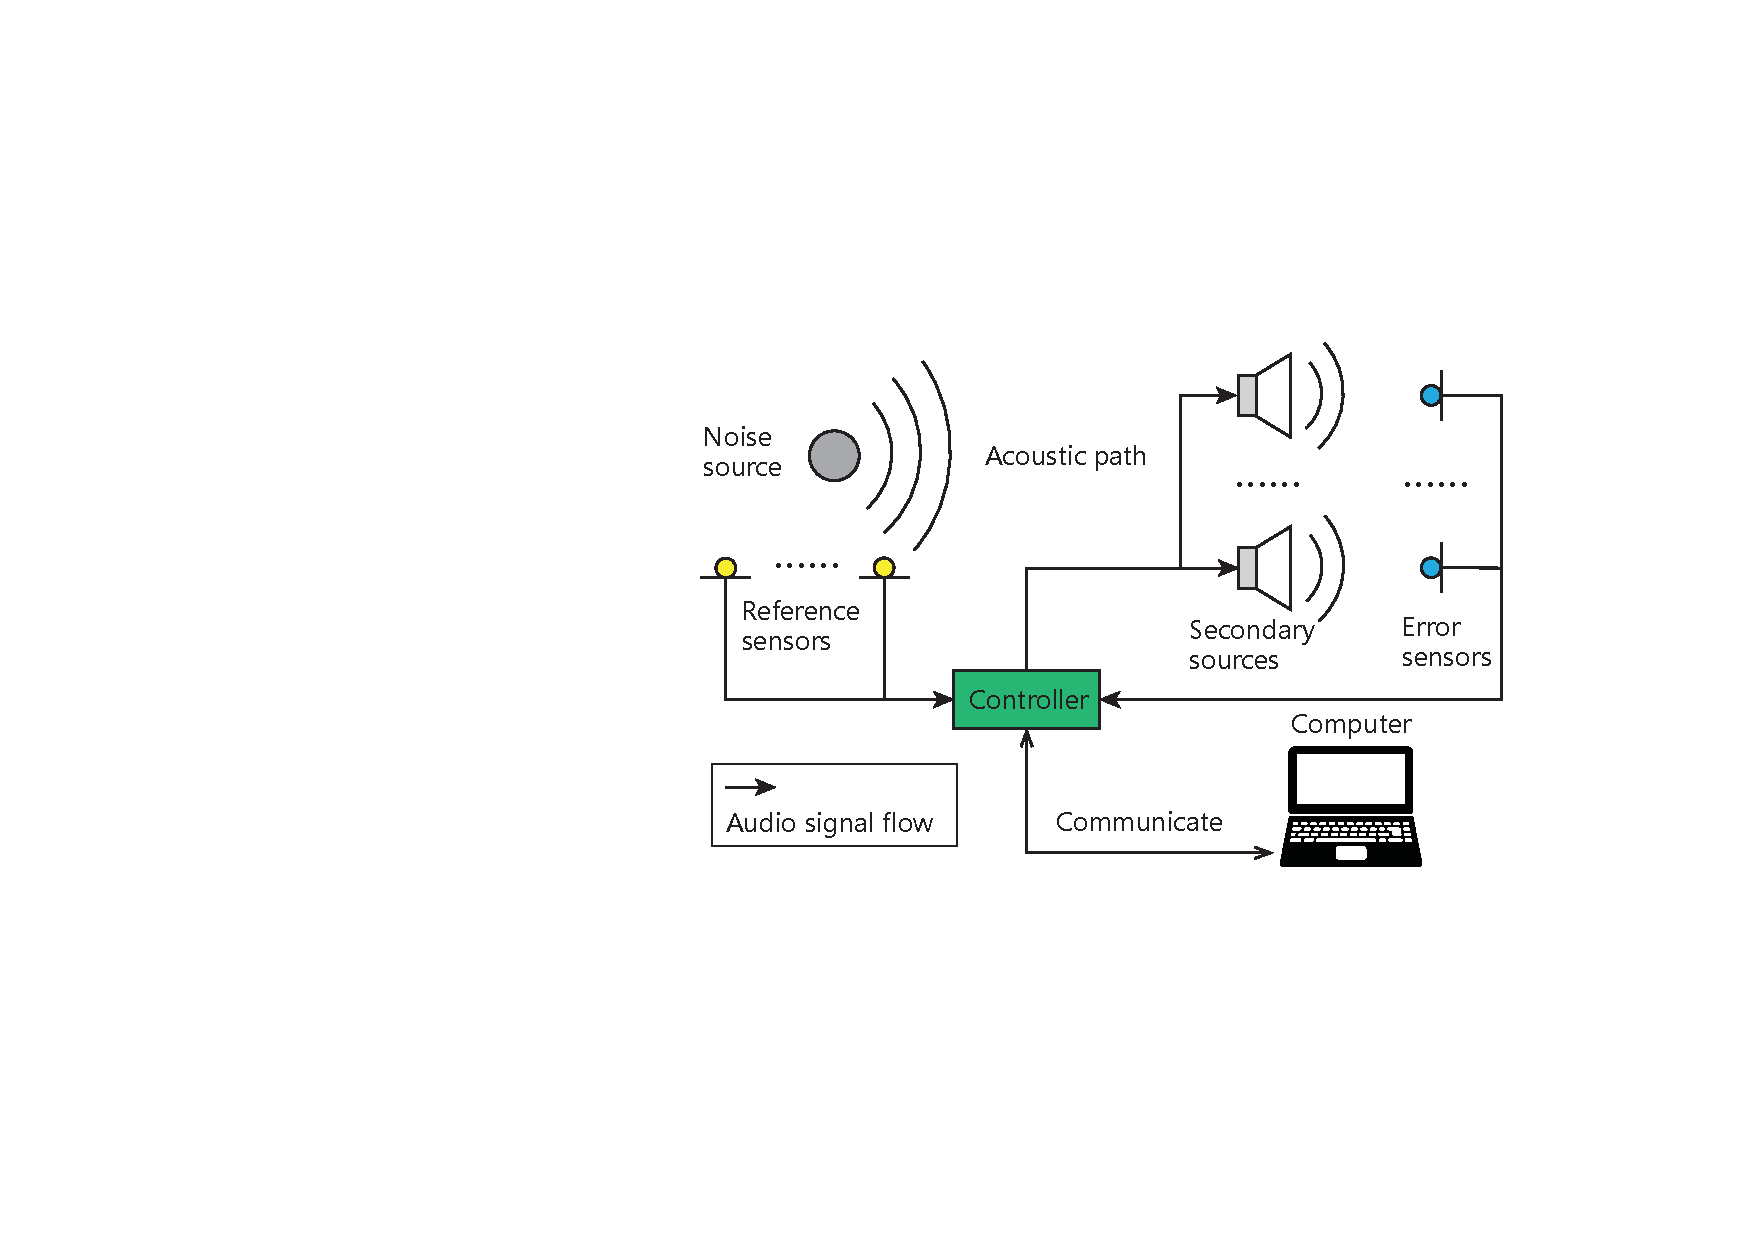
\includegraphics[width = 0.6\textwidth]{fig/ANC_structure/ANC_structure_211117A.pdf}
    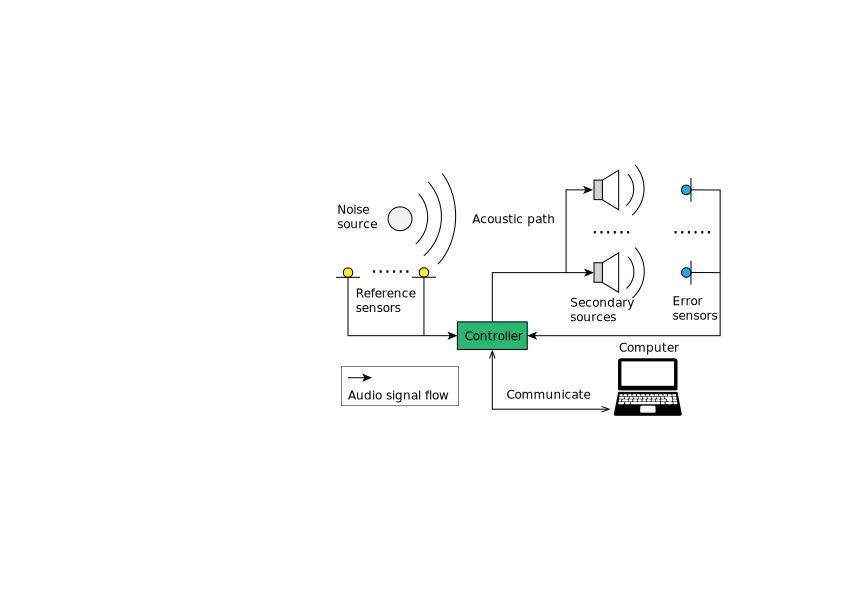
\includegraphics[width = 0.6\textwidth]{fig/ANC_structure/ANC_structure_211117A.png}
    \caption{Structure of an ANC system.}
    \label{fig:anc_structure}
\end{figure}

%% todo: insert a figure to show the examples mentioned above

    There are two strategies of ANC systems, namely global active control and local active control \cite{Nelson1992ActiveControlSound}.
    The global active control aims to reduce the total sound power radiated from the noise and secondary sources \cite{Boodoo2015ReviewEffectReflective}. 
    Although the radiation of the system can be globally mitigated when the distance between secondary and noise sources is small, the noise reduction performance deteriorates significantly when the distance is larger than half of a wavelength \cite{Zhong2019IncreasingPerformanceActive, Zhong2019IncreasingPerformanceActivea, Zhong2020PerformanceActiveNoise}.
    When global control cannot be achieved, local active control can be used to mitigate the noise in a particular region and form a so called \quotes{quiet zone}, which is defined as the region where the noise reduction is larger than 10 dB \cite{Guo1998EffectsReflectiveGround, Elliott2015ModelingLocalActive, Shi2020MultichannelActiveNoise}.
    It is noted that the sound field in other areas is not taken into account in the local active control strategy.
    When the traditional dynamic loudspeakers are used as secondary sources in ANC systems, 
    the noise in some other areas outside the quiet zone can be amplified 
    because traditional dynamic loudspeakers are approximately omnidirectional.
    This phenomenon is referred to as the \quotes{spillover effect} in the literature \cite{Guo1997ActivelyCreatedQuiet, Kidner2006FeasibilityStudyLocalised, Tanaka2010ActiveNoiseControl}.

To illustrate the spillover effect, Fig.~\ref{fig:intro:389fsdp} is presented showing the physical configuration of a single channel ANC system.
When a secondary source (denoted by a cross mark) is used to cancel the noise radiated by a point source (denoted by a circle mark) at an error point (denoted by a square mark), 
the quiet zone is formed around the error point.
The spillover effect can be observed that the sound pressure in some other areas is amplified due to the omnidirectional sound waves generated by the traditional secondary loudspeakers, which is undesirable in real applications.
Moreover, such property increases the instability of the ANC system because the reference signal is contaminated by the secondary source signal received by the reference sensors \cite{Tanaka2010ActiveNoiseControl}. 
As shown in Fig.~\ref{fig:anc_change_dist}, placing the secondary source close to the target point can mitigate the increase of total energy in the other areas \cite{Joseph1994FieldZonesQuiet, David1994NumericalStudiesActively}, 
but it reduces the quiet zone size \cite{Guo1998EffectsReflectiveGround}, 
and also brings extra obstructions to the target point.
    The spillover effect is annoying in applications.
    For example, when a quiet zone is created in the main driver's seat inside a car cabin, the occupants sitting in other seats experience the noise amplification \cite{Cheer2012ActiveControlAcoustic, Jung2018MidfrequencyLocalActive}. 
    It is therefore desirable to manipulate the secondary sound waves so that they propagate only in the direction of error points.

\begin{figure}[!htb]
    \centering
    \begin{subfigure}{0.49\textwidth}
        \centering
        % \includegraphics[width = 1\textwidth]{E:/Research/InterNoise2020/m/ANC/fig/cal_ANC_demo_Off_1kHz_resize.jpg}
        % \includegraphics[width = 1\textwidth]{E:/Research/InterNoise2020/matlab/ANC/fig/cal_ANC_demo_Off_1kHz_resize.jpg}
        \includegraphics[width = 1\textwidth]{fig/cal_ANC_demo_Off_1kHz_resize.jpg}
        \caption{}
    \end{subfigure}
    \begin{subfigure}{0.49\textwidth}
        \centering
        % \includegraphics[width = 1\textwidth]{E:/Research/InterNoise2020/matlab/ANC/fig/cal_ANC_demo_On_1kHz_SecPointMonopole_dse4m_resize.jpg}
        \includegraphics[width = 1\textwidth]{fig/cal_ANC_demo_On_1kHz_SecPointMonopole_dse4m_resize.jpg}
        \caption{}
    \end{subfigure}
    \caption{\revA{Sound pressure level (SPL; dB re 20 $\mu$Pa)} generated by a point source located at $(x,z) = (0,\SI{6}{m})$ at 1 kHz: (a) primary (noise) field; (b) the noise at the $(x,z) = (0,0)$ is controlled by introducing a secondary source at $(x,z) = (0, \SI{4}{m})$. 
        Circle, primary source; cross, secondary source; square, error point. 
    }
    \label{fig:intro:389fsdp}
\end{figure}

\begin{figure}[!htb]
    \centering
    \begin{subfigure}{0.49\textwidth}
        \centering
        \includegraphics[width = 1\textwidth]{fig/cal_ANC_demo_On_1kHz_SecPointMonopole_dse0p5m_resize.jpg}
        \caption{}
    \end{subfigure}
    \begin{subfigure}{0.49\textwidth}
        \centering
        \includegraphics[width = 1\textwidth]{fig/cal_ANC_demo_On_1kHz_SecPointMonopole_dse2m_resize.jpg}
        \caption{}
    \end{subfigure}
    \caption{\revA{SPL (dB re 20 $\mu$Pa)} generated by a point source located at $(x,z) = (0,\SI{6}{m})$ at 1 kHz and the sound at the $(x,z) = (0,0)$ is controlled by a traditional omnidirectional loudspeaker at: (a) $(x,z) = (0, \SI{0.5}{m})$; and (b) $(x,z) = (0,\SI{2}{m})$. Circle, primary source; cross, secondary source; square, error point.}
    \label{fig:anc_change_dist}
\end{figure}

% The single channel ANC system shown in Figs. \ref{fig:intro:389fsdp} and \ref{fig:anc_change_dist} can creat only one
% If multiple quiet zones or a larger quiet zone 
    The spillover effect is also occurred in the  multi-channel local active control system, which aims to create multiple quiet zones or a larger quiet zone using multiple secondary sources \cite{Nelson1992ActiveControlSound}. 
    For example for a binaural ANC system as shown in Fig.~\ref{fig:intro:tanaka2017model}, two secondary sources are introduced to mitigate the noise at two ears.
    The secondary field at each ear is the superposition of the sound waves radiated by two secondary loudspeakers.
    Except for two secondary paths between either loudspeakers and the ipsilateral ears, there are another two crosstalk secondary paths between either loudspeakers and the contralateral ears.
    If the secondary source is omnidirectional, the crosstalk secondary paths are non-negligible and must be taken into account in signal processing algorithms. 
    They would double the computational cost in the ANC controller \cite{Tanaka2017BinauralActiveNoise}.

\begin{figure}[!htb]
    \centering
    \includegraphics[width = 0.5\textwidth]{Figures/pending/Tanaka2017-Model_resize.jpg}
    \caption{Sketch of a binaural ANC system using two PALs. From Fig. 6 in \cite{Tanaka2017BinauralActiveNoise}.}
    \label{fig:intro:tanaka2017model}
\end{figure}


% Some studies have demonstrated the capabilities and potentials of using directional sources to eliminate the spillover effect \cite{Mangiante1977ActiveSoundAbsorption, Chen2011ActiveNoiseBarrier, Hu2019ActiveCancellationSound}. 
The sound waves radiated by directional sources focus on their propagation axis, and have small effects in other directions.
Owing to this feature, using directional sources in ANC systems can mitigate the spillover effect \cite{Mangiante1977ActiveSoundAbsorption, Chen2011ActiveNoiseBarrier, Hu2019ActiveCancellationSound} as well as reduce the crosstalk secondary paths \cite{Tanaka2014MultichannelActiveNoise, Tanaka2017BinauralActiveNoise}. 
Parametric array loudspeakers (PALs) are a special kind of loudspeakers, which has sharp radiation directivity when compared to existing traditional dynamic loudspeakers. %, and is therefore a promising secondary source for ANC systems. 
The sharp directivity for PALs can be clearly identified in a comparison of the sound field radiated by a PAL and a traditional loudspeaker of the same radiation surface, as shown in  Fig.~\ref{fig:pal_sound_field_compare_to_traditional}.
The advantage of using PALs in ANC systems has been demonstrated in some studies \cite{Tanaka2010ActiveNoiseControl, Tanaka2011MathematicallyTrivialControl, Tanaka2014MultichannelActiveNoise, Tanaka2017BinauralActiveNoise}. 
For example, after replacing the omnidirectional secondary source in Fig.~\ref{fig:anc_change_dist} by the PAL, the noise reduction performance is shown in Fig.~\ref{fig:anc_change_dist_pal} and , it is clear the spillover effect is much reduced.
However, most existing studies focus on using one or two PALs to cancel the noise at error points, where the generated quiet zone is rather small.
It is necessary to investigate the feasibility of using multiple PALs to generate a large quiet zone.

\begin{figure}[!htb]
    \centering
    \begin{subfigure}{0.47\textwidth}
        \centering
        % \includegraphics[width=\textwidth]{E:/UTS/CandidatureAssessment/CA1/slides/img/show_2D_audio1000_PistonSource_A_resize.jpg}
        \includegraphics[width=\textwidth]{fig/show_2D_audio1000_PistonSource_A_resize.jpg}
        \caption{}
    \end{subfigure}
    \begin{subfigure}{0.47\textwidth}
        \centering
        % \includegraphics[width=\textwidth]{E:/UTS/CandidatureAssessment/CA1/slides/img/show_2D_audio1000_ultra60e3_A_resize.jpg}
        \includegraphics[width=\textwidth]{fig/show_2D_audio1000_ultra60e3_A_resize.jpg}
        \caption{}
    \end{subfigure}
    \caption{\revA{SPL (dB re 20 $\mu$Pa)} at 1 kHz generated by: (a) a traditional loudspeaker; (b) a PAL located at the origin and of the same radiation surface.}
    \label{fig:pal_sound_field_compare_to_traditional}
\end{figure}

\begin{figure}[!htb]
    \centering
    \begin{subfigure}{0.49\textwidth}
        \centering
        \includegraphics[width = 1\textwidth]{fig/cal_ANC_demo_On_1kHz_SecPAL_dse2m_resize.jpg}
        \caption{}
    \end{subfigure}
    \begin{subfigure}{0.49\textwidth}
        \centering
        \includegraphics[width = 1\textwidth]{fig/cal_ANC_demo_On_1kHz_SecPAL_dse4m_resize.jpg}
        \caption{}
    \end{subfigure}
    \caption{
        \revA{SPL (dB re 20 $\mu$Pa)} generated by a point source located at $(x,z) = (0,\SI{6}{m})$ at 1 kHz and the sound at the $(x,z) = (0,0)$ is controlled by a PAL at: (a) $(x,z) = (0, \SI{0.5}{m})$; and (b) $(x,z) = (0,\SI{2}{m})$. 
    \revA{Circle, primary source; cross, secondary source; square, error point.}}
    \label{fig:anc_change_dist_pal}
\end{figure}

    ANC and related audio systems are used in various kinds of acoustic environments, where the sound waves experience the reflection, transmission, scattering, and other physical phenomena. 
    % These properties have significant effects on the noise reduction performance of ANC systems.
    When traditional dynamic loudspeakers are adopted as secondary sources, they are usually modelled as point monopoles at low frequencies, the theory of which is trivial. 
    At middle and high frequencies, more accurate models can be used to predict the sound field, such as the model taking into account the radiation directivity or the aperture size of the loudspeakers.
    The theory for traditional dynamic loudspeakers has been well developed and used in investigating the effects of the physical properties of secondary sources on ANC performance.
    For example, it has been demonstrated that the noise reduction performance can be much improved by optimally setting the locations of secondary sources and reflecting surfaces for both global and local active control \cite{Boodoo2015ReviewEffectReflective, Tao2017PerformanceMultichannelActive, Zhong2019IncreasingPerformanceActive, Zhong2019IncreasingPerformanceActivea, Zhong2020PerformanceActiveNoise};
    the ANC system can be used to increase the insertion loss of a passive partition \cite{Sas1995ActiveControlSound, Tarabini2009ActiveControlNoisea, Zhang2017PerformanceSnoringNoise} and enclosures \cite{Dupont2009ActiveAbsorptionReduce};
    the scattering effects caused by a human head is beneficial to the ANC system in terms of performance robustness with regard to the movements of the human head \cite{Lin2004ActiveControlRadiation, Zou2008PerformanceAnalysisVirtual, Liu2018ActiveControlStrategy, Elliott2020ActiveControlSound}.
    All of aforementioned studies demonstrate the physical properties (e.g., reflection, transmission, and scattering) of secondary sources have significant effects on the performance of ANC systems.
    % However, The generation of audio sound by a PAL is a nonlinear process, and the theory is more complicated than the traditional loudspeakers.
    However, these properties for audio sound generated by PALs are still unclear, which will be investigated in this thesis.
    % The active partition (a passive partition integrated with an ANC system) can increase the insertion loss of the partition

% For the applications in the field of ANC, it is necessary to know the physical properties of the sound waves generated by secondary sources in various kinds of acoustic environments, such as the reflection from a reflecting surface \cite{Boodoo2015ReviewEffectReflective, Tao2017PerformanceMultichannelActive, Zhong2019IncreasingPerformanceActive, Zhong2019IncreasingPerformanceActivea, Zhong2020PerformanceActiveNoise}, transmission through a partition \cite{Sas1995ActiveControlSound, Tarabini2009ActiveControlNoisea, Zhang2017PerformanceSnoringNoise}, and scattering by a human head \cite{Lin2004ActiveControlRadiation, Zou2008PerformanceAnalysisVirtual, Liu2018ActiveControlStrategy, Elliott2020ActiveControlSound}. 
% Although the theoretical research on predication models for the audio sound generated by a PAL has continued to date (e.g., \cite{Shi2012ProductDirectivityModels, Shi2015ConvolutionModelComputing, Cervenka2013NonparaxialModelParametric, Guasch2018FarfieldDirectivityParametric, Cervenka2019VersatileComputationalApproach} for details), there are still a lot to do to improve the calculation efficiency and accuracy for PALs in different acoustic environments. 

\section{Objectives}
% This thesis focuses on the investigation of prediction models, physical properties of audio sound generated by a PAL, and the applications in ANC systems as secondary sources to create a large quiet zone.
% The objectives of this thesis lie in the following three aspects in the field of PAL and ANC.
The primary aim of this thesis is to investigate the feasibility of using multiple PALs in an ANC system to create a large quiet zone.
This thesis aims to improve the fundamental understanding of how PALs affect the noise reduction performance and the quiet zone size in a multi-channel ANC systems.
In particular, since heavy computations for the audio sound generated by PALs are required in modelling the noise reduction performance of a multi-channel ANC system, a new partial-wave expansion method is proposed to reduce the computational load without causing loss of accuracy. 
In addition, the proposed method is extended to investigate the reflection, transmission, and scattering phenomena for PALs, which are common in real applications but the relevant studies are rare.
Finally, the proposed model incorporated with the multi-channel ANC theory is used to investigate the quiet zone size controlled by multiple PALs.
The spillover effect will be evaluated quantitatively and compared to the systems using traditional dynamic loudspeakers which have omnidirectional radiation pattern.

% \noindent\paragraph{Objective 1}\mbox{}\\

% The accurate calculation of audio sound generated by a PAL is rather time-consuming due to the evaluations of five-fold integrals \cite{Cervenka2019VersatileComputationalApproach}. 
% The existing method employs the paraxial (Fresnel) approximation to simplify the calculations which is inaccurate at wide angles from the radiation axis of the PAL \cite{Cervenka2013NonparaxialModelParametric}. 
% Therefore, it is worth investigating whether it is possible to simplify the calculation without additional approximations. 
% The existing method is based on a baffled model; however, it has been reported that audio sound can be heard behind a PAL in free field (non-baffled model). 
% It is necessarily to develop a theoretical model which can predict the sound on both front and back sides of a non-baffled PAL.

% \noindent\paragraph{Objective 2}\mbox{}\\

% The audio sound generated by PALs can be treated as the superposition of the sound generated by infinitely many virtual sources in space with the source density proportional to the product of the sound pressure of ultrasound. 
% Therefore, the formation of the audio sound is accumulated before the ultrasound being totally absorbed in air. 
% There would be interesting phenomena if the accumulation process is truncated by a reflecting surface, blocked by a partition, or scattered by a sphere (simulating a human head).
% The results and conclusions are also useful for applications of PALs in ANC systems.

% \noindent\paragraph{Objective 3}\mbox{}\\

% It has been reported that PALs can be used in ANC systems to create a quiet zone around the target point without affecting the sound levels in the other areas. 
% However, the existing studies focus only on the control of the pure tone or  narrow band (upper limit is less than 2.5 kHz) noise \cite{Tanaka2010ActiveNoiseControl, Tanaka2014MultichannelActiveNoise, Tanaka2011MathematicallyTrivialControl, Tanaka2017BinauralActiveNoise}.
% The feasibility of applying PALs to reduce broader band noise up to 6 kHz remains to be investigated, as well as the feasibility of creating a large quiet zone with multiple PALs.


\section{Thesis outline}
The structure of the thesis is as follows:

\noindent\paragraph{Chapter \ref{chap:intro}: \nameref{chap:intro}}\mbox{}\\

This chapter gives a brief introduction on the concepts of PAL and ANC, and the motivation and objectives of this thesis.
The thesis outline and contributions are also presented.

\noindent\paragraph{Chapter \ref{chap:review}: \nameref{chap:review}}\mbox{}\\

This chapter presents a systematic review of PAL and ANC.
For PALs, it includes the physical mechanism and properties of the audio sound generated by a PAL, 
the prediction models, implementations and applications. 
For ANC, it includes the methods to generate a quiet zone and ANC systems using directional loudspeakers and PALs.

\noindent\paragraph{Chapter \ref{chap:sound_field}: \nameref{chap:sound_field}}\mbox{}\\

This chapter firstly reviews the governing equations for audio sound generated by a PAL.
The quasilinear solutions for both three-dimensional and two-dimensional models are presented.
The front side for a baffled PAL is proposed to be divided into three regions: the near field, the Westervelt far field, and the inverse-law far field.
The widely used \revA{Gaussian beam expansion (GBE)} model and the convolution model are concluded to predict the sound fields in the Westervelt far field and the inverse-law far field, respectively.
The sound field on the back side for a non-baffled PAL is predicted using the non-paraxial PAL model and the disk scattering theory.
Experimental results are presented to validate the proposed model.

\noindent\paragraph{Chapter \ref{chap:predict_model}: \nameref{chap:predict_model}}\mbox{}\\

This chapter proposes two improved prediction models for PALs.
The first model is called the \revA{spherical wave expansion (SWE)} model which is used to calculate the radiation from a circular piston source, and the audio sound generated by a circular PAL.
The second model is called the \revA{cylindrical wave expansion (CWE)} model which is used to calculate the audio sound generated by a phased array PAL.
The advantages of the proposed models are illustrated by numerical simulations.

\noindent\paragraph{Chapter \ref{chap:phys}: \nameref{chap:phys}} \mbox{}\\

This chapter provides a systematic investigation on the physical properties for audio sound generated by a PAL.
The reflection of audio sound generated by a PAL is investigated first when an infinitely large reflecting surface is placed near the PAL. 
A theoretical model is then developed to predict the transmission of audio sound generated by a PAL through a thin partition, and is used to quantitatively analyze the insertion loss. 
The scattering effects of a rigid sphere (simulating a human head) on audio sound generated by a PAL are investigated.
Experimental results are presented to validate the models proposed in this chapter.

\noindent\paragraph{Chapter \ref{chap:anc}: \nameref{chap:anc}} \mbox{}\\

This chapter investigates the feasibility of using a PAL to reduce a broadband (up to 6 kHz) noise at the human ears.
Then the feasibility of using multiple PALs to create a large quiet zone is investigated, and the physical limitations are explored. 
Experiments of both single and  multi-channel ANC systems are conducted to verify the findings.

\noindent\paragraph{Chapter \ref{chap:conclusion}: \nameref{chap:conclusion}} \mbox{}\\

This chapter concludes the work in this chapter.
The future work and outlook are also presented. 

\section{Contributions}
The main original contributions of this thesis are as follows:
\begin{outline}[enumerate]
    \1 A spherical wave expansion method for calculating the audio sound generated by a PAL has been proposed for both Westervelt \cite{Zhong2020SphericalExpansionAudio} and Kuznetsov \cite{Zhong2021FieldWesterveltFar} equations.
    The proposed method is found to be not only more accurate but also 15 times faster than the widely used Gaussian beam expansion method, and is more than 100 times faster than the direct integration method without any loss of accuracy.
    \1 A closed-form solution for calculating the radiation from a circular piston source has been proposed using the spherical wave expansion method \cite{Zhong2020SphericalExpansionCalculating}.
    \1 A cylindrical wave expansion method for calculating the audio sound generated by a phased array PAL has been proposed \cite{Zhong2021CylindricalExpansionAudio}.
    It improves the agreement with the experimental results when compared to the existing convolution model.
    \1 The reflection from a reflecting surface \cite{Zhong2020ReflectionAudioSounds}, the transmission through a thin partition \cite{Zhong2020InsertionLossThin}, and the scattering by a rigid sphere (simulating a human head) \cite{Zhong2022ScatteringRigidSphere}, for audio sound generated by a PAL have been investigated by both simulations and experiments.
    The work provides a framework and a guidance for investigating these physical properties of audio sound generated by a PAL.
    \1 An ANC system has been designed and implemented to cancel the noise at human ears, where the secondary source is a commercial PAL and the error signal is remotely detected by an optical microphone using the laser Doppler vibrometer technique \cite{Zhong2020ExperimentalStudyActive}.
    Experiments are conducted to test the performance of such a system.
    \1 The feasibility of using multiple PALs to create a large quiet zone has been validated by both simulations and experiments \cite{Zhong2022QuietZoneGeneration}.
    The empirical formulae to estimate the quiet zone size have been proposed.
\end{outline}


\chapter{Literature Review} % Main chapter title

\label{chap:review} % Change X to a consecutive number; for referencing this chapter elsewhere, use \ref{ChapterX}

%----------------------------------------------------------------------------------------
%	SECTION 1
%----------------------------------------------------------------------------------------
This chapter presents a literature review on PALs and ANC in Secs.  \ref{sec:literature_pal} and \ref{sec:review_anc}, respectively.
The physical mechanisms and the basic properties of the PAL are introduced in Sec.~\ref{sec:literature_pal_phys}.
The governing equations and existing prediction models are reviewed in Sec.~\ref{sec:review_pal_predict}.
Implementations and applications of the PAL are presented in \ref{sec:review_implement}.
The approaches and algorithms to realize an ANC system are introduced in Sec.~\ref{sec:anc_algorithm}.
The mechanism of the quiet zone generation for an ANC system is introduced in Sec.~\ref{sec:review_anc_qz}.
The ANC system using directional loudspeakers and PALs are reviewed in Secs. \ref{eq:review_anc_directional} and \ref{sec:review_anc_pal}, respectively.

\section{Parametric array loudspeakers (PALs)}
\label{sec:literature_pal}

\subsection{Physical mechanisms}
\label{sec:literature_pal_phys}
It is well known that a sound wave distorts as it propagates, and this can be seen as a nonlinear interaction of the sound wave with itself \cite{Hamilton2008NonlinearAcoustics}. 
If there are two sound waves of frequencies $f_1$ and $f_2$ with $f_1>f_2$, it is expected that four components of these frequencies: $2f_1, 2f_2,f_1\pm f_2$ {will be generated when} subject to the second-order nonlinearity, where the component of frequency $f_1-f_2$ is known as the difference frequency wave (DFW). 
The occurrence of these components has been demonstrated and observed in many studies, and this nonlinear phenomenon is known as \quotes{the scattering of sound by sound}, although it usually refers to the generation of DFW outside the nonlinear interaction region \cite{Ingard1956ScatteringSoundSound, Westervelt1957ScatteringSoundSound, Westervelt1957ScatteringSoundSounda, Bellin1960ScatteringSoundSound, Darvennes1990ScatteringSoundSound, Dimant2021LensMediatedScattering}. 
There are also further studies and applications on utilizing the higher order nonlinear components \cite{Qian1995NonlinearAcousticsHigherorder, Ma2006ThirdOrderHarmonic, Liu2007TheoreticalExperimentalStudy, Mitri2010NonlinearAcousticsHigherorder, Garner2012ThirdorderParametricArray, Johnson2014EfficientApproachComputing, Garner2011DesignOptimalDirectional}.

Enlightened by these findings, Westervelt {was the first to propose} the concept of {parametric acoustic array} (PAA) in 1963 \cite{Westervelt1963ParametricAcousticArray}. 
When a PAA radiates two collimated primary sound waves of frequencies $f_1$ and $f_2$, a DFW that has sharp directivity is generated {at a frequency of $f_1 - f_2$}.
As shown in Fig.~\ref{fig:lr:89fjsd}, 
{the second-order nonlinear effects cause such a beam to act like a distribution of virtual sources for the DFW \cite{Westervelt1960ParametricEndFire}. 
    The source density of these virtual sources is proportional to the amplitude of the primary waves, which is approximately exponentially attenuated along the propagation axis (end-fire direction of the virtual source array \cite{Berktay1973NearfieldEffectsEndfire}).
    These sources form a so-called \quotes{end-fire array} with a semi-infinitely long length \cite{Gan2012ReviewParametricAcoustic}, which can produce low frequency directional sound beams in the end-fire direction without side lobes \cite{Bellin1962ExperimentalInvestigationEnd, Mellen1976NearfieldBeamPatterns, Mellen1977NearfieldAxialLevels, Tu2016RobustnessCompactEndfire}.
}
% the virtual sources of the DFW are generated along the propagation path of the primary wave to form an end-fire array \cite{Gan2012ReviewParametricAcoustic}. 
% Therefore, the DFW is highly directional even though its frequency is low \cite{Berktay1973NearfieldEffectsEndfire}.

\begin{figure}[h]
    \centering
    \includegraphics[width = 0.7\textwidth]{fig/gan2012_paa_sketch_resize.png}
    \caption{Demonstration of the generation of audible sound beam by using the PAA. From Fig.~1 in \cite{Gan2012ReviewParametricAcoustic}.}
    \label{fig:lr:89fjsd}
\end{figure}

The PAA was firstly used in underwater applications, such as sub-bottom profiling \cite{Humphrey2008AcousticCharacterizationPanel, Qu2018ExperimentalStudyBroadband}, underwater communications \cite{Wiedmann2012ParametricUnderwaterCommunications}, detection of buried objects \cite{Trucco2000AcousticDetectionObjects}, and so on; a review can be found in \cite{Zhou2020ParametricAcousticArray}.
The application of PAA in air is called {a} PAL, where the primary sound and DFW correspond to ultrasonic and audio waves, respectively.
The parametric effect in air was firstly experimentally observed by Bennett and Blackstock in 1975 \cite{Bennett1975ParametricArrayAir}.
{This work was followed by Yoneyama et al.\ who} designed and fabricated a new type of loudspeaker based on {the principles of PAA} \cite{Yoneyama1983AudioSpotlightApplication}.
{
    They used 547 PZT bimorph ultrasonic transducers with the center frequency of 40 kHz to generate the audio sound from 200 Hz to 20 kHz, and sharp directivity patterns for audio waves were observed in measurements as expected. 
}
Although it is called the \quotes{audio spotlight} in their work (shown in Fig.~\ref{fig:298jfjdsjdjfj}), it is more often called a PAL in {the literature}. 
They also showed the demodulated wave has a rate of 12 dB/octave decrease as the frequency is halved. 
However, it is possible to get a flat response for the reproduced audio sound generated by the PAL by using an equalizer. 

\begin{figure}[!htb]
    \centering
    \includegraphics[width = 0.35\textwidth]{fig/yoneyama1983_audio_spotlight_resize.png}
    \caption{Front view of the first audio spotlight (PAL). From Fig.~2 in \cite{Yoneyama1983AudioSpotlightApplication}.}
    \label{fig:298jfjdsjdjfj}
\end{figure}


Although PALs are capable of generating narrow beams at low frequencies, 
the amplitude of the beams decreases slightly with distance, which is a disadvantage in some appliations. 
{
    For example, the audio beam at 1 kHz radiated by a PAL with the dimensions of $\SI{60}{cm} \times \SI{60}{cm}$ attenuates only around 6 dB at the distance of 4 m on the propagation axis \cite{HolosonicsResearchLabs2018AudioSpotlightTechnical}.
This means undesirable multiple reflections from walls and floor would happen when using PALs in a room.
% After multiple reflections, the sound waves can be perceived in almost every direction, so the sharp directivity 
% The reflected sound beams decay slowly, so the 
Recently, a so-called \quotes{length-limited PAL} is proposed which can produce audible sound only in a limited range in front of the transducer \cite{Hedberg2010SelfsilencedSoundBeam}.
The idea is to cancel out the sound generated by the PAL by using another PAL of different carrier frequency producing audible sound of equal amplitude but in anti-phase.
A finite-difference time-domain (FDTD) method was proposed to numerically model the sound propagation generated by an axisymmetric length-limited PAL \cite{Nomura2012NumericalSimulationParametric}. 
Their simulation results shown in Fig.~\ref{fig:nomuera:LLPAL} demonstrate the feasibility of realization of such a length-limited PAL, where the audible sound decreases rapidly at the axial distance of 2 m.
Skinner and et al.\  used pairs of commercial off the shelf PAL and conducted a series of measurements to assess the practicality of a length-limited PAL \cite{Skinner2019DemonstrationLengthLimited}. 
}

\begin{figure}[!htb]
    \centering
    \includegraphics[width = 0.5\textwidth]{fig/lengthlimitedPAL_resize.png}
    \caption{Contour lines indicate the SPL normalized by each maximum level from $-6$ to 0 dB in steps of 1 dB. The carrier frequencies for sources 1 and 2 are 77 kHz and 52 kHz, respectively. From Fig.~10 in \cite{Nomura2012NumericalSimulationParametric}.}
    \label{fig:nomuera:LLPAL}
\end{figure}

{
    Except for limiting the audio sound in the near field of the PAL, there are also studies in remotely creating an audio spot \cite{Ye2008GenerationAudibleSound, Ji2009InvestigationLocalizedSound, Matsui2013DesignAudioSpot, Iijima2019AudioHotspotAttack}.
    As shown in Fig.~\ref{fig:92sdjfjj}, the idea of this technique is to emit the carrier wave ($f_1$) and sideband wave ($f_2$) by two separated PALs. 
    The two sound beams are inaudible along their propagation path because they are ultrasonic waves.
    However, the sound in the overlap region of these two sound beams is audible due to the parametric nonlinear interactions between them.
    Therefore, a small locally audible space is remotely created.
    This feature enables delivering the sound secretely and has been used to \quotes{attack} (performs a secret malicious voice command) the voice assistance system, such as Siri, Google Assistant, and Amazon Alexa \cite{Iijima2019AudioHotspotAttack}.
    % therefore remotely create a 
    % The sound become audible only in the overlap region of these two sound beams. 
}

\begin{figure}[!htb]
    \centering
    \includegraphics[width = 0.4\textwidth]{fig/Ijima2019.png}
    \caption{Audio spot creation using two PALs. From Fig.~1 in \cite{Iijima2019AudioHotspotAttack}.}
    \label{fig:92sdjfjj}
\end{figure}


\subsection{Prediction models}
\label{sec:review_pal_predict}
{
    Accurate and computationally efficient prediction model for PALs is necessary in simulating the performance of ANC and other related audio systems using PALs.
}
The fundamental model is a baffled circular PAL installed on an infinitely large reflecting surface \cite{Cervenka2013NonparaxialModelParametric}. 
When a PAL radiates two intensive ultrasonic waves at different frequencies, a secondary wave containing the DFW (the audio sound in air) is generated due to the {second-order} nonlinearity.
The nonlinear interactions of primary waves are rather complex, and some approximations and simplifications have to be made in the mathematical modelling.
Because the ultrasound level generated by a PAL is limited for safety concerns \cite{Gan2012ReviewParametricAcoustic, Lawton2001DamageHumanHearing, Pompei2002SoundUltrasoundParametric}, the nonlinearity is {normally} weak and the quasilinear approximation is usually assumed.
By expanding the sound field up to second-order under the quasilinear assumption, 
one {then} obtains a set of hierarchical linear wave equations for both the ultrasound and the audio sound \cite{Hamilton2008NonlinearAcoustics, Silva2013DifferencefrequencyGenerationNonlinear}.
{This enables the ultrasound to} be modelled as the radiation from a planar source, so the field can be obtained using the well-known Rayleigh integral.
The audio sound {is then} seen as radiation from an infinitely large volume source with the source density proportional to the product of the {ultrasonic} pressure.

\paragraph{Far field}\mbox{}\\ % \label{sec:literature_pal_far}
The calculation of audio sound pressure in the far field is of great interest because the expression of the solution is usually much simpler and can be used to analyze the directivity of the PAL \cite{Shi2014OverviewDirectivityControl}.
The first closed-form expression for audio beam directivity was proposed in Westervelt's seminal work, and this is usually termed the Westervelt directivity \cite{Westervelt1963ParametricAcousticArray}.
In this model, it is assumed that the ultrasonic waves are collimated and fully attenuated in the near field of the PAL, and the audio sound is seen to be generated by a line array of virtual sources with the source density exponentially decreasing along the radiation axis of the PAL \cite{Westervelt1963ParametricAcousticArray}. 
{The solution demonstrates the sharp directivity of the PAL.}
However, large differences between predictions obtained using Westervelt's directivity and experimental measurements have been reported \cite{Shi2014OverviewDirectivityControl}, and this is thought to be because {of the} assumptions in the {original} model.

Many attempts have been made to improve the accuracy of the directivity predictions.
Berktay \cite{Berktay1965PossibleExploitationNonlinear} and Berktay and Leahy \cite{Berktay1974FarfieldPerformanceParametric} modified Westervelt's directivity by taking into account effects arising from the cylindrical/spherical spreading of ultrasonic waves, and they improved prediction accuracy by introducing an aperture factor for the transducer and the product directivity of ultrasonic waves. 
The Berktay's solution is given as a simple expression in the time domain, which provides the basis for the signal modulation techniques in the realization of PALs \cite{Gan2012ReviewParametricAcoustic, Shi2016VolterraModelParametric}.
Berktay described the generation of the audio sound as a self-modulated process, so the audio sound is sometimes referred to as the demodulated signal.
Several modifications to the Berktay model were later proposed to improve the prediction accuracy for the sidelobes of PALs \cite{Shi2012ProductDirectivityModels}.

The most accurate approach to date for the far field prediction is to employ the convolution of the ultrasonic wave directivities and Westervelt's directivity \cite{Shi2015ConvolutionModelComputing, Guasch2018FarfieldDirectivityParametric, Shi2022ExtendedConvolutionModel}.
An arbitrary directivity for the ultrasound can then be set in the convolution model to calculate the audio sound directivity, and reported experimental results have demonstrated that it outperforms other existing models in the far field for a steerable PAL \cite{Shi2014OverviewDirectivityControl, Shi2015ConvolutionModelComputing}. 
However, the ultrasound beams are assumed to be exponentially attenuated in each direction, which is not true in reality because of the complexity of the ultrasound beams in the near field, where the majority of the nonlinear interactions take place. 
Furthermore, the far field is usually more than 10 m away from a PAL when its size is larger than 0.04 m \cite{Moffett1981NearfieldCharacteristicsParametric, Zhong2021FieldWesterveltFar}, which is too far when compared to real applications. 
Therefore, differences between predictions and measurements continue to be observed, even for the sound pressure 4 m away from the PAL \cite{Shi2015ConvolutionModelComputing}.


% \subsubsection{Near field}
% Many governing equations have been proposed to calculate the near field audio sound.
% In early studies, the Lighthill equation is commonly used in the mathematical modelling which  is derived from conservation of mass and conservation of momentum \cite{Lighthill1952SoundGeneratedAerodynamically, Westervelt1963ParametricAcousticArray}.
% Combining with the equation of state and ignoring cubic and higher terms, the second-order nonlinear wave equation is obtained \cite{Aanonsen1984DistortionHarmonicGeneration, Cervenka2019VersatileComputationalApproach}.


\paragraph{KZK equation}\mbox{}\\
It has been shown {that} the aforementioned far field solution %in Sec.~\ref{sec:literature_pal_far} 
is inaccurate to predict the near field audio sound \cite{Zhong2021FieldWesterveltFar}.
Several governing equations have been proposed to obtain more accurate results in the near field.
In early studies, the most widely used model is based on the Khokhlov-Zabolotskaya-Kuznetsov (KZK) equation, which is a second-order model and considers the diffraction, absorption and nonlinearity of both the ultrasonic and {the} audio sound waves \cite{Zabolotskaya1969QuasiplaneWavesNonlinear, Kuznetsov1971EquationsNonlinearAcoustics, Hamilton2008NonlinearAcoustics}.

Various kinds of methods have been proposed to numerically solve {the} KZK equation in both frequency \cite{Aanonsen1984DistortionHarmonicGeneration, Kamakura1989NonlinearlyGeneratedSpectral, Kamakura1992HarmonicGenerationFinite} and time \cite{Lee1993NumericalSolutionKZK, Averkiou1993SelfDemodulationAmplitude} domains.
The paraxial (Fresnel) approximation is assumed for both the ultrasound and the audio sound in KZK equation, so it is valid only in the vicinity of the propagation axis, approximately 20 degrees  from the transducer axis  \cite{Hamilton2008NonlinearAcoustics}. 
The solution based on {the} KZK equation is therefore called \quotes{the paraxial solution}.
This approximation is generally acceptable for ultrasound because the ultrasonic wavelength (e.g., 8.6 mm at 40 kHz) is usually much smaller than the aperture size of the PAL. 
However, the prediction for audio sound is inaccurate because the audio sound wavelength is much larger (e.g., 34.3 cm at 1 kHz), and the error increases as the audio frequency decreases \cite{Cervenka2013NonparaxialModelParametric}.
In addition, the KZK equation is difficult {to use when calculating} the sound propagation in complex environments, such as the reflection, transmission, and/or scattering, {where the accuracy is known to reduce} \cite{Li2019NumericalExperimentalStudies}.

\paragraph{Westervelt equation}\mbox{}\\
A more accurate governing equation is called the Westervelt equation.
Actually, the KZK equation can be seen as a parabolic approximation of the Westervelt equation, which is applicable in the paraxial region {only} \cite{Aanonsen1984DistortionHarmonicGeneration, Cervenka2013NonparaxialModelParametric}.
In this model, the ultrasound is calculated first {using} a two-fold Rayleigh integral over the area of the transducer surface. 
{Next}, the audio sound is calculated by a three-fold integral over the full space of the product of the source density (determined by ultrasound field) and the Green's function for a point source.
This {approach results in} a five-fold integral and {this can be} very time-consuming to {solve} \cite{Zhong2020SphericalExpansionAudio}.

To simplify the calculation, the Gaussian beam expansion (GBE) method is usually used {as this} simplifies the two-fold integral required for both the ultrasound and the audio sound \cite{Wen1988DiffractionBeamField, Cervenka2013NonparaxialModelParametric}.
The GBE method approximates the vibration velocity profile of the transducer surface by {using} multiple Gaussian functions.
Because the radiation from a planar source that has a Gaussian profile has the closed-form solution under the paraxial (Fresnel) approximation, the calculation of ultrasound field is then simplified by a superposition of the radiation from multiple Gaussian beams.
If the radiation surface for the planar surface is circular, {then} the two-fold integral can be simplified by a one-fold summation.
It has been shown that various kinds of velocity profiles can be approximated by Gaussian beams using the optimization theory \cite{Wen1988DiffractionBeamField, Ding1996SimpleCalculationApproach, Ding2000SimplifiedAlgorithmSecondorder, Ding2003ExtensionsGaussianBeam, Ding2004SimplifiedAlgorithmSecondorder, Ding2004NotesGaussianBeam, Ding2005SupplementaryNotesGaussian, Cervenka2015StructureMultiGaussianBeam}. 

% PAA
In addition {to a} planar source {with} a circular surface, the GBE method can also be used for {a} source that has other shapes, such as rectangular and elliptical, and the two-fold integral is simplified by a two-fold summation \cite{Ding2003ExtensionsGaussianBeam, Ding2004NotesGaussianBeam, Ding2005SupplementaryNotesGaussian}.
They are then extended for calculation of the audio sound generated by a rectangular PAL \cite{Jun2004FastFieldScheme, Yang2005ModelingFiniteamplitudeSound, Masunaga2012HarmonicDistortionMeasurement} and the array of PAL consisting of circular elements \cite{Ye2010ModelingParametricLoudspeakers}.
In early studies, the GBE method is applied for both the ultrasound and the audio sound, and the prediction accuracy is therefore {equivalent to} that {obtained using the} KZK equation \cite{Ye2010ModelingParametricLoudspeakers}.
In 2013, Cervenka and Bednařík employed the GBE only for the ultrasound and {obtained} a more accurate solution, which is called \quotes{the non-paraxial model} \cite{Cervenka2013NonparaxialModelParametric}.

% cons
The GBE model assumes the paraxial approximation, and some extensions on this model have been proposed which is applicable in the non-paraxial region \cite{Zhao2009NonparaxialMultiGaussianBeam, Wang2017TwodimensionalAnalyticModeling}.
Although the GBE method consumes less calculation time than the direct integration approach, the Gaussian functions are not a complete set so it is not an exact solution of the Westervelt equation under the quasilinear approximation. 
Furthermore, Gibbs oscillations occur for a uniform piston source no matter how many Gaussian beams are used \cite{Wen1988DiffractionBeamField, Cervenka2015StructureMultiGaussianBeam}, and the calculation of the off-axis audio sound is still time consuming due to the triple-integral over the whole space.

\paragraph{Kuznetsov equation}\mbox{}\\
Even {if} the five-fold integral based on the Westervelt equation is calculated without additional approximations, the {predictions} can be inaccurate when the so-called \quotes{local effects} are dominant in the nonlinear interactions of {the} ultrasound \cite{Aanonsen1984DistortionHarmonicGeneration}.
In this case, the process can be modelled using a second-order nonlinear wave equation if cubic and higher order terms are neglected \cite{Aanonsen1984DistortionHarmonicGeneration}.
The Lagrangian density, which characterizes the local effects, is contained in this equation {and}, it reduces to {the} Westervelt equation if the Lagrangian density is neglected. 
However, this equation is rarely used in numerical calculations due to the difficulty of {evaluating the} spatial second derivatives of the Lagrangian density \cite{Kagawa1992FiniteElementSimulation}.
Instead, the Kuznetsov {equation} is more convenient, which is identical to the second-order nonlinear equation but is expressed in terms of the velocity potential \cite{Aanonsen1984DistortionHarmonicGeneration, Cervenka2019VersatileComputationalApproach}.
For a progressive plane wave, it has been shown {that} the influence of the Lagrangian density is small enough to be neglected at field points away from the PAL. 
However, the accuracy is reduced significantly at points close to the PAL \cite{Cervenka2019VersatileComputationalApproach}.


\subsection{Implementation and applications}
\label{sec:review_implement}

{The} implementation of a PAL consists of 4 parts, which are 
the ultrasonic emitter, the power amplifier, the signal processor, and the peripheral circuit.
As shown in Fig.~\ref{fig:Gan2012AA:block_diagram}, 
the audio signal is fed into a signal processor and it is modulated with carrier (ultrasonic) signals based on various kinds of modulation algorithms \cite{Yoneyama1983AudioSpotlightApplication, Matsui2013DesignAudioSpot, Shi2016EffectUltrasonicEmitter}.
After passing through the power amplifier, the modulated signal is radiated by the ultrasonic emitter and the audio sound is then demodulated (generated) in air due to the parametric effect.

\begin{figure}[htb]
    \centering
    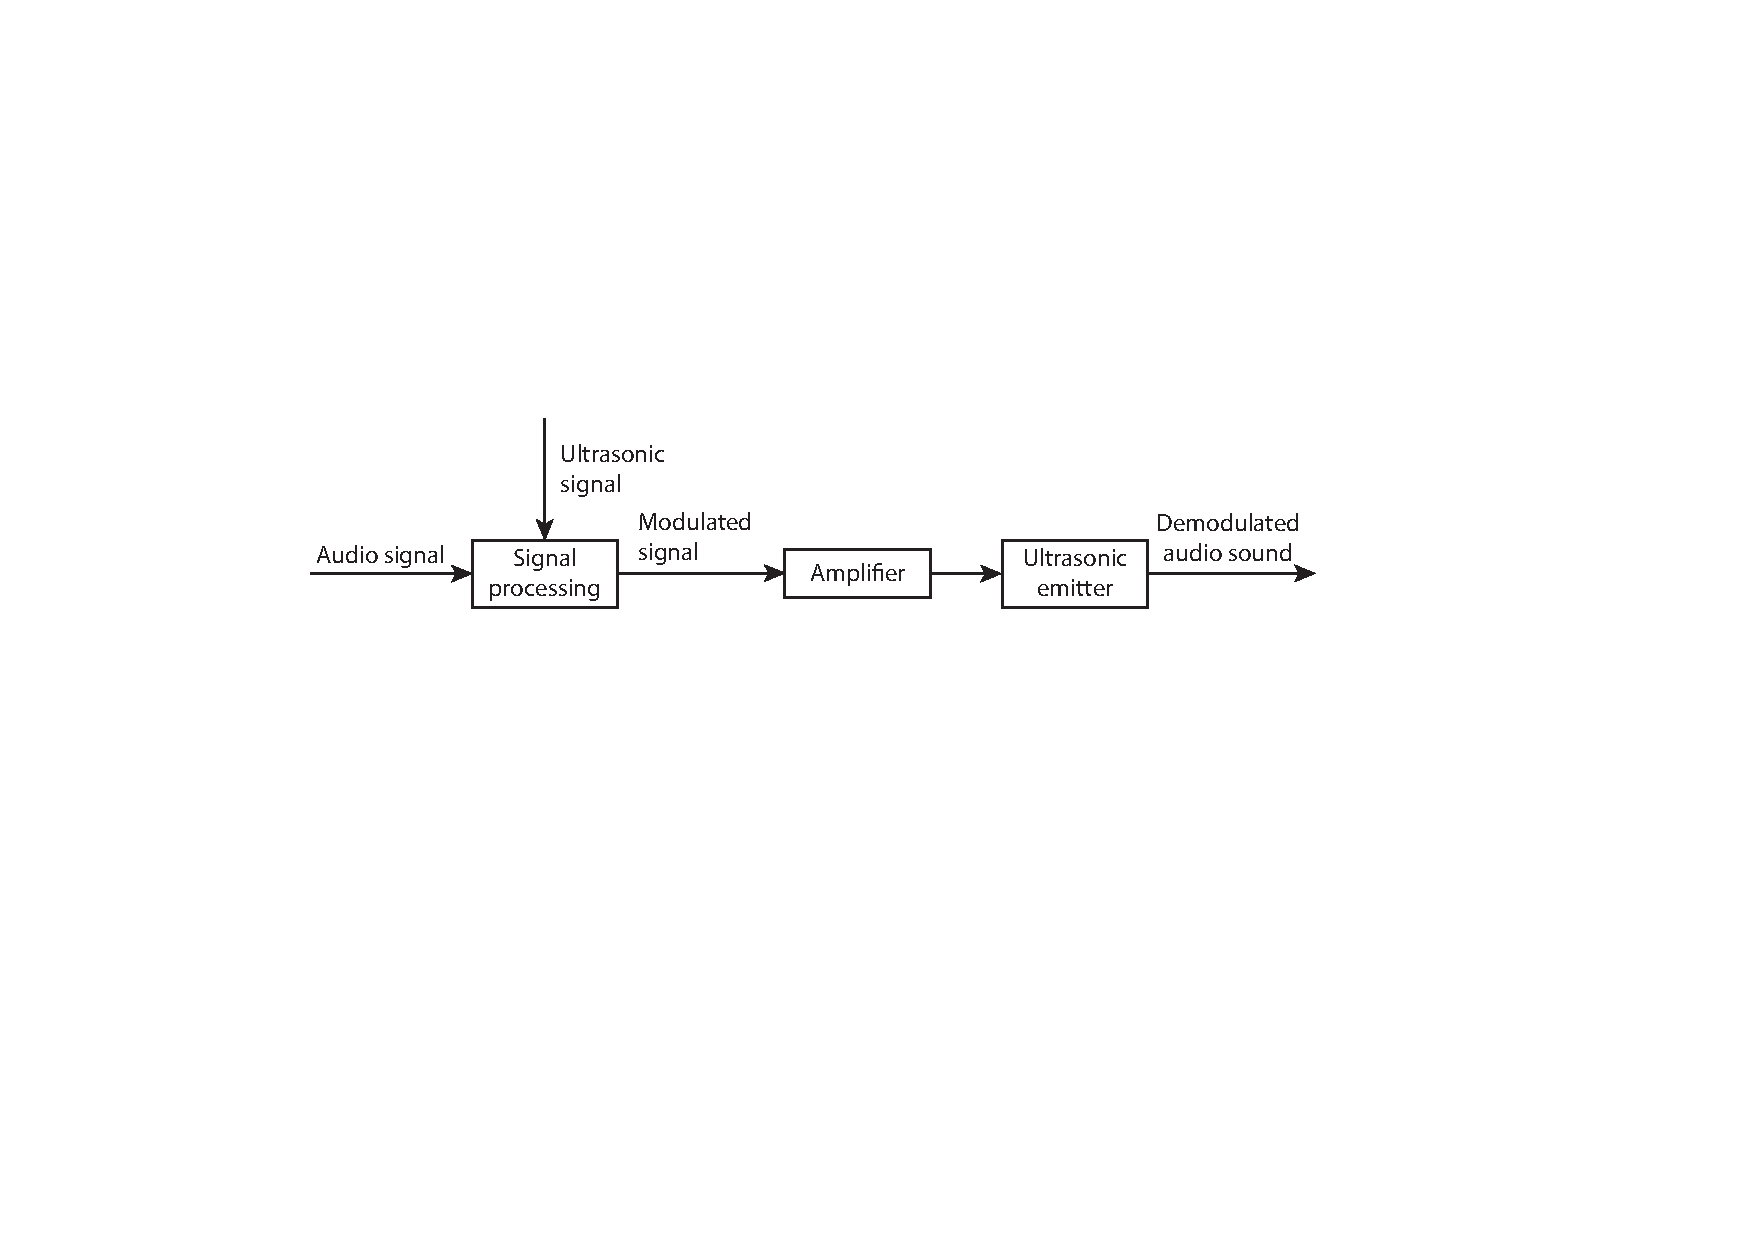
\includegraphics[width = 0.85\textwidth]{fig/Gan2012_PAL_block_diagram/Gan2012_PAL_block_diagram.pdf}
    \caption{Block diagram of the implementation of a PAL. From Fig.~11 of \cite{Gan2012ReviewParametricAcoustic}.}
    \label{fig:Gan2012AA:block_diagram}
\end{figure}
% 考虑是否加入传统换能器的对比
\paragraph{Ultrasonic emitter}\mbox{}\\
The piezoelectric transducers are the most common ultrasonic emitters used in PALs. 
Table~\ref{tab:eifsdf} and Fig.~\ref{fig:flksdafsdf} present some commercial emitters.
It is found the emitter type MA40S4S from Murata is the most popular one.

\begin{table}
    \centering
    \begin{tabular}{cccc}
        \toprule
        Model & Company & \makecell{Center frequency} & Used in \\
        \midrule
        Airducer AT-50 & AirMar & 50 kHz & \cite{Hedberg2010SelfsilencedSoundBeam, Johnson2016ModulationRadioFrequency}\\
        Airducer AT-75 & AirMar & 75 kHz & \cite{Hedberg2010SelfsilencedSoundBeam}\\
        FBULS1007P-T & Ningbo Best Group Factory & 40 kHz& \cite{Marzo2017TinyLevMultiemitterSingleaxis}\\
        MA40H1S-R & Murata & 40 kHz & \cite{Jager2019AirborneUltrasoundPhased}\\
        MA40S4S & Murata & 40 kHz& \cite{Marzo2017TinyLevMultiemitterSingleaxis, Hahn2021ParametricArrayUsing, Jager2019AirborneUltrasoundPhased, Marzo2017UltrainoOpenPhasedarray,Sayin2013RealizationOmnidirectionalSource, Sayin2013DirectivityControlEfficiency, Ji2019ExperimentalInvestigationParameters, Shi2013InvestigationSteerableParametric, Tseng2018PhasedArrayFocusing, Hirayama2019VolumetricDisplayVisual}\\
        MCUSD16A40S12RO & MultiComp & 40 kHz& \cite{Marzo2017TinyLevMultiemitterSingleaxis}\\
        MCUST10P40B07RO & MultiComp & 40 kHz& \cite{Marzo2017TinyLevMultiemitterSingleaxis, Arnela2018ConstructionOmnidirectionalParametric, Arnela2021CharacterizationOmnidirectionalParametric}\\
        MSO-A1625H12T & Manorshi & 25 kHz & Not found\\
        MSO-P1640H10TR &  Manorshi & 40 kHz& \cite{Marzo2017TinyLevMultiemitterSingleaxis}\\
        MSO-A1640H10T & Manorshi & 40 kHz& \cite{Marzo2017TinyLevMultiemitterSingleaxis}\\
        MSO-P1040H07T & Manorshi & 40 kHz& \cite{Marzo2017TinyLevMultiemitterSingleaxis}\\
        T4010B4 & Nippon Ceramic & 40 kHz & \cite{Ochiai2017HolographicWhisperRendering}\\
        ZT40-16 & Shanghai Nicera Sensor & 40 kHz & \cite{Ji2016DevelopmentAcousticFilter, Ji2019ExperimentalInvestigationParameters}\\
        \bottomrule
    \end{tabular}
    \caption{Commercial ultrasonic emitters.}
    \label{tab:eifsdf}
\end{table}

\begin{figure}[!htb]
    \centering
    \begin{subfigure}{0.3\textwidth}
        \centering
        \includegraphics[width = \textwidth]{fig/20211226022137_resize.png}
        \caption{Murata MA40S4S. From Fig.~2.17(a) in \cite{Jager2019AirborneUltrasoundPhased}. }
    \end{subfigure}
    \qquad
    \begin{subfigure}{0.3\textwidth}
        \centering
        \includegraphics[width = \textwidth]{fig/20211226022344_resize.png}
        \caption{Murata MA40H1S-R. From Fig.~2.17(b) in \cite{Jager2019AirborneUltrasoundPhased}. }
    \end{subfigure}
    \caption{Commercial ultrasonic emitters.}
    \label{fig:flksdafsdf}
\end{figure}

The electroacoustic efficiency is usually very low for traditional ultrasonic emitters. 
The main reason is the large acoustic impedance mismatch between air ($\SI{415}{Rayls}$) and the emitter (e.g., $\SI{34}{MRayls}$ for PZT4) \cite{Gallego-Juarez1978UltrasonicTransducerHigh}.
A promising approach is to reduce the characteristic mechanical impedance of the emitter by using a {thin-film} structure, which can be fabricated using the micromachined technique \cite{Lee2009MicromachinedSourceTransducer}.
Piezoelectric micromachined ultrasonic transducers (PMUTs) are compact and efficient emitters for PALs .
Lee et al.\ designed and fabricated a PMUT and the electroacoustic efficiency is measured {to be} 21.9\% \cite{Lee2009MicromachinedSourceTransducer}.
Later, they improved the efficiency to 58.4\% \cite{Je2013ImpactMicromachinedUltrasonic} and {then} 71\% \cite{Je2015MicromachinedEfficientParametric}.
Furthermore, the PMUT has a wide bandwidth, and a $\pm\SI{3}{dB}$ bandwidth of 17 kHz was reported for the ultrasonic waves \cite{Je2015MicromachinedEfficientParametric}.


\paragraph{Power amplifier}\mbox{}\\
The class D amplifier is usually used due to its high efficiency in electroacoustic conversion \cite{Stark2007DirectDigitalPulse}.
Early implementation of PALs use{d} analog circuits, see \cite{Pompei2002SoundUltrasoundParametric} for example. 
Modern PALs are adopting digital circuits, where the digital signal processor (DSP) and field programmable gate array (FPGA) are usually used as the signal processor. 
Karnapi et al.\ designed and implemented a PAL system in FPGA platform using the Altera 1S10 device \cite{Karnapi2004FPGAImplementationParametric}.
{
    Recently, the metal-oxide-semiconductor field-effect transistor (MOSFET) is introduced to amplify the ultrasonic emitters \cite{Marzo2017UltrainoOpenPhasedarray, Hahn2021ParametricArrayUsing}. 
    In 2021, a phased array PAL was realized by Hahn et al.\ using a microcontroller and MOSFET drivers \cite{Hahn2021ParametricArrayUsing}. 
    It is showed that the switching mechanism of the MOSFETs benefit to the signal processing and steering the sound beam.
}

\paragraph{Signal processing methods}\mbox{}\\
The audio signal cannot be radiated by the ultrasonic emitter directly, {as} it has to be modulated into ultrasonic signals via signal processors.
A fundamental preprocessing technique is the amplitude modulation, which is usually called the double sideband (DSB) amplitude modulation in {the literature} \cite{Yoneyama1983AudioSpotlightApplication}.
However, the lower and upper sideband introduced in the DSB amplitude modulation suffer from interference which causes distrotions. 
The single sideband (SSB) modulation method was proposed, where a quadrature path is used to cancel the nonlinear distortion \cite{Aoki1991ParametricLoudspeakerCharacteristics}. 
Kamakura et al.\ proposed the square root (SRT) modulation method in 1984, which can be used to eliminate all of the undesired harmonics theoretically \cite{Kamakura1984DevelopmentsParametricLoudspeaker}.
However, the SRT modulation method requires an ideal ultrasonic emitter that has a perfect flat response (i.e., infinite bandwidth to produce the square-root), which is impossible in real implementations \cite{Shi2016EffectUltrasonicEmitter}.
The effects of the ultrasonic emitter on the distortion performance for different modulation methods {are} compared and reviewed in \cite{Shi2016EffectUltrasonicEmitter}.
A more practical technique called modifield amplitude modulation was proposed based on the quadrature amplitude modulation \cite{Gan2008DistortionAnalysisReduction, Tan2010PreprocessingTechniquesBandlimited, Ji2010TheoreticalExperimentalComparison, Tan2010PreprocessingTechniquesBandlimited}.

In addition to the efforts on eliminating the harmonic distortion, 
signal processing techniques are used to equalize the frequency response of the PAL.
According to the Berktay's far field solution \cite{Berktay1965PossibleExploitationNonlinear}, there is a decrement of 12 dB/octave in the frequency response of the audio sound generated by a PAL \cite{Yoneyama1983AudioSpotlightApplication}.
In 1998, Kite et al.\ proposed a method to equalize by introducing a double integral \cite{Kite1998ParametricArrayAir}.
More concerns are focuesd on the virtual bass enhancement, which is a psychoacoustic signal processing technique enhancing the low frequency sound by adding the harmonics of the fundamental frequency \cite{Arora2006LowComplexityVirtual, Karnapi2002MethodEnhanceLow, Gan2010AudioProjectionDirectional, Shi2013PsychoacousticalPreprocessingTechnique}. 

\paragraph{Applications and commercial products}\mbox{}\\
The PAL has attracted much attention in audio applications because of its sharp directivity, small size, and negligible sidelobes compared to the traditional loudspeakers.
Due to these advantages, PALs have been widely used in applications including ANC systems \cite{Tanaka2010ActiveNoiseControl, Tanaka2011MathematicallyTrivialControl, Tanaka2014MultichannelActiveNoise, Tanaka2017BinauralActiveNoise}, 
personal communications \cite{Nakashima2005PrototypeParametricArray}, 
museum exhibitions and service and multimedia booths \cite{Kortbek2008CommunicatingArtInteractive}, 
measurement of the acoustic parameters of materials \cite{Castagnede2006ReflectionTransmissionNormal, Castagnede2008LowFrequencySitu}, 
mobile robotic navigation \cite{Skinner2019DemonstrationLengthLimited},
stand-off concealed weapons detection \cite{Rudd2008SimulationIncidentNonlinear},
directivity control \cite{Shi2014OverviewDirectivityControl}, 
constructions of omnidirectional loudspeakers \cite{Arnela2018ConstructionOmnidirectionalParametric, Arnela2021CharacterizationOmnidirectionalParametric},
sound reproduction systems \cite{Alunno2017DirectionalLandscapesUsing};
and many other areas.
The applications of PALs in ANC systems will be introduced in detail in Sec.~\ref{sec:review_anc_pal}.
{Due to its potential in audio applications, some commercial PALs are available on the market and presented in Table \ref{tab:pal_commercial_product} and Fig.~\ref{fig:pal_commercial_product}.
}

\begin{table}[H]
    \centering
    \begin{tabular}{lll}
        \toprule
        Model & Company & Country\\
        \midrule
        Audio Spotlight & Holosonics & USA \\
        Hypersound & Turtle Beach Corporation& France\\
        MSP-50E & Mistubishi Electric Engineering Company & Japan\\
        Acouspade speaker &  Ultrasonic Audio Technologies& Slovenia\\
        Focusound directional speaker & Audfly Technology (Suzhou) & China \\
        Soundlazer & Richard Haberkern & USA\\
        \bottomrule
    \end{tabular}
    \caption{Commercial products of the PAL.}
    \label{tab:pal_commercial_product}
\end{table}
\begin{figure}[!htb]
    \centering
    \begin{subfigure}{0.3\textwidth}
        \centering
        \includegraphics[width=\textwidth]{fig/CommercialProducts/As-24i.png}
        \caption{Audio Spotlight AS-24i from \cite{HolosonicsAudioSpotlight24i}}
    \end{subfigure}
    \hfill
    \begin{subfigure}{0.3\textwidth}
        \centering
        \includegraphics[width=\textwidth]{fig/CommercialProducts/Hypersound_resize.png}
        \caption{HyperSound HSS3000 from \cite{TurtleBeachCorporationHyperSoundHSS300}}
    \end{subfigure}
    \hfill
    \begin{subfigure}{0.2\textwidth}
        \centering
        \includegraphics[width=\textwidth]{fig/CommercialProducts/MSP-50E_resize.png}
        \caption{MST-50E from \cite{MitsubishiElectricMSP050E}}
    \end{subfigure}
    \\
    \begin{subfigure}{0.35\textwidth}
        \centering
        \includegraphics[width=\textwidth]{fig/CommercialProducts/Acouspade-directional-Sound-Speaker_resize.jpg}
        \caption{Acouspade from \cite{UltrasonicAudioTechnologiesACOUsticSPAceDElimiter}}
    \end{subfigure}
    \hfill
    \begin{subfigure}{0.3\textwidth}
        \centering
        \includegraphics[width=\textwidth]{fig/CommercialProducts/FocusoundModelR.jpg}
        \caption{Focusound Model R from \cite{2021ProductsDescriptionsFocusound}}
    \end{subfigure}
    \hfill
    \begin{subfigure}{0.2\textwidth}
        \centering
        \includegraphics[width=\textwidth]{fig/CommercialProducts/Soundlazer_resize.png}
        \caption{Soundlazer SL-01 from \cite{2021SoundlazerPuttingSound}}
    \end{subfigure}
    \caption{Several commercial products of the PAL.}
    \label{fig:pal_commercial_product}
\end{figure}

% The earliest applications for PAAs lie in sonar \cite{Berktay1965ParametricAmplificationUse, Browning2009ParametricAcousticArray, Ostrovsky2009ResearchParametricArrays}.

%----------------------------------------------------------------------------------------
%	SECTION 2
%----------------------------------------------------------------------------------------

\section{Active noise control (ANC)}
\label{sec:review_anc}

Lueg {was the first to introduce} the concept of an ANC system{, which was reported} in a US patent granted in 1936 \cite{Lueg1936ProcessSilencingSound}.
It demonstrated the cancellation of a sound field can be realized by superimposing an electroacoustically generated secondary sound field that has an opposite phase \cite{Lueg1936ProcessSilencingSound, Guicking1990InventionActiveNoise}.
Early ANC applications focused on the control of noise radiated by a transformer \cite{Ross1978ExperimentsActiveControl}.
Nowadays, more and more applications are reported, and the theory and signal processing techniques can be found in textbooks \cite{Nelson1992ActiveControlSound, Fuller1996ActiveControlVibration, Elliott2000SignalProcessingActive, Hansen2012ActiveControlNoise, Kuo1996ActiveNoiseControl}.
In general, there are two types of ANC systems: the global and the local active control.
For a global control system, the aim is to reduce the total radiation from the noise source.
However, it is possible and practical only when the secondary source is close to the noise source (smaller than half of the wavelength) \cite{Nelson1992ActiveControlSound}.
Therefore, local control is more popular which aims to create a small quiet zone at target regions \cite{Joseph1994FieldZonesQuiet}.
This section focuses on the review of {approaches and algorithms to realize an ANC system}, the quiet zone generation, and existing ANC systems using directional loudspeakers and PALs.

\subsection{Approaches and algorithms}
\label{sec:anc_algorithm}
{
Depending on the use of reference sensors, the ANC system can be classified as the feedforward strcture and the feedback structure \cite{Elliott2000SignalProcessingActive}. 
Figure~\ref{fig:anc_structure} shows the feedforward structure of an ANC system, where the reference sensors are placed near the noise source to acquire the primary noise.
The anti-noise control signal emitted by the secondary sources is calculated based on the reference signal.
It goes through the secondary path (the acoustic path from the secondary source and the error point) and entirely cancels the primary nosie at the error sensors.
The residual error signal at error sensors is used to dynamically adjust the output of the control signal enabling the maximum noise reduction. 
\revA{A disadvantage of the feedforward structure is that the reference signal is affected by the sound radiated by the secondary source when the reference signal is recorded by the acoustic based sensors (e.g., microphones)}, which makes the system unstable \cite{Akhtar2007ActiveNoiseControl}.
This can be solved by using directional loudspeakers as secondary sources so that the secondary sound waves do not propgate in the direction of the reference sensors.
Compared to the feedforward strucutre, the feedback structure does not need reference sensors. 
Instead, the information of the primary noise is captured from the error signal.
Although the feedback structure requires less sensors than the feedforward structure, 
it is hard to predict broadband signals due to the limitation of system causility, so it is only used to deal with the narrowband noise \cite{Elliott2000SignalProcessingActive}.
The feedforward ANC is more stable and used in applications, and it is therefore adopted in this thesis.
}

{
% The approach to implementing a feedforward ANC system is to 
It is hard to implement a feedforward ANC system using analog circuits. 
Digital processors with adaptive filter algorithms are generally used nowadays.
The aim of the adaptive filter algorithm in an ANC controller is to find the control filter which enables the maximum noise reduction at error sensors. 
There are various kinds of algorithms to obtain the control filter, while the FxLMS is the most practical one,
and also used in commercial ANC controllers \cite{Shi2020AlgorithmsImplementationsOvercome, Antysound2017TigerANCWiFiQUserManual}.
The mechanism of FxLMS algorithm can be illustrated by Fig.~\ref{fig:98sdjf83j}.
$P(z)$ and $S(z)$ represent the path from the primary noise and secondary srouce to the error point, respectively.
$\hat{S}(z)$ is an estimation of $S(z)$. 
The reference signal denoted by $x(n)$ is filtered by the control filter $W(z)$ and becomes the control signal $y(n)$.
The control filter $W(z)$ is adaptively updated according to the minimize the square of the error signal $e(n)$.
There are also other algorithms to improve the convergence speed and reduce the computational cost of the control filter, such as the normalized FxLMS algorithm \cite{Slock1993ConvergenceBehaviorLMS, Shi2015IdentificationParametricArray}; a more detailed review can be found in \cite{Shi2020AlgorithmsImplementationsOvercome}.
}
\begin{figure}[!htb]
    \centering
    \includegraphics[width = 0.7\textwidth]{fig/shi2019_fxlms.png}
    \caption{Block diagram of the FxLMS algorithm. From Fig.~2.3 in \cite{Shi2020AlgorithmsImplementationsOvercome}.}
    \label{fig:98sdjf83j}
\end{figure}



\subsection{Quiet zone generation}
\label{sec:review_anc_qz}
{The} ANC technique is effective {in controlling a noise source} at the error point. 
However, it only creates a small quiet zone around the error point, and the quiet zone is usually defined as the region where the noise reduction is larger than 10 dB \cite{Elliott2015ModelingLocalActive}. 
Furthermore, the size of the quiet zone becomes smaller as the frequency increases.
For an ANC system with one secondary source, the size of the quiet zone is only about one tenth of the wavelength in a diffuse sound field \cite{Guo1998EffectsReflectiveGround, Elliott1988ActiveCancellationPoint}. 
The challenge to be addressed with ANC involves maximizing the size of {this} quiet zone. 

To enlarge the quiet zone, 
a multi-channel ANC system that has multiple secondary sources and error microphones is usually used  \cite{Zhang2019ActiveNoiseControl}. 
The sound pressure inside a closed surface surrounded by multiple secondary sources can be controlled if the spacing between the secondary sources is sufficiently small \cite{Elliott2018WavenumberApproachAnalysing}. 
In a free field, the quiet zone size is found to be proportional to the number of secondary sources \cite{Guo1997ActivelyCreatedQuiet}.
Experimental measurements show that more than 20 dB of noise reduction can be obtained inside a sphere with a radius of 0.3 m for frequencies from 100 Hz and 500 Hz, when using 30 secondary sources on a spherical surface \cite{Epain2007ActiveControlSound}.
In an ordinary room, experimental results with 16 secondary sources distributed over a cylindrical surface demonstrate that a cylindrical quiet zone with a height of 0.2 m and a radius of 0.2 m is possible below 550 Hz \cite{Zou2007PreliminaryExperimentalStudy}. 
A large quiet zone usually requires a larger number of secondary sources and error microphones, so 
{recent work has focused on} reducing the number of microphones \cite{Maeno2018ModeDomainSpatial} and loudspeakers \cite{Zhang2016MultichannelActiveNoise}. 

In these ANC systems, omnidirectional loudspeakers were used as secondary sources. 
Although the noise inside the target region is reduced, the sound pressure outside the region often increases, which is known as the spillover effect \cite{Guo1997ActivelyCreatedQuiet, Tanaka2010ActiveNoiseControl}. 
{This causes} noise amplification outside the target areas, {which} can be mitigated by optimizing some parameters such as the separation between the secondary sources and the distance between secondary sources and {the} error sensors \cite{Guo1997ActivelyCreatedQuiet, Joseph1994FieldZonesQuiet, David1994NumericalStudiesActively}.
To address this problem, directional loudspeakers have been shown to have the potential to lower this external sound field \cite{Tanaka2010ActiveNoiseControl, Hu2019ActiveCancellationSound}. 
PALs have sharper directivity than most traditional dynamic loudspeakers \cite{Gan2012ReviewParametricAcoustic}, but the feasibility of using them to create a quiet zone is not clear, and so this will be investigated here.

\subsection{ANC using directional loudspeakers}
\label{eq:review_anc_directional}
The type of secondary source in an ANC system is crucial for {delivering high levels of} noise reduction \cite{Bolton1995SoundCancellationUse, Qiu2000SecondaryAcousticSource}.
{It is common for a single monopole, or an array of monopoles, to be used as secondary sources in ANC systems}.
However, directional sources can be used as secondary sources in multiple channel ANC systems to improve performance. 
For example, tripole secondary sources with a cardioid radiation pattern have been used to reduce noise source radiation \cite{Mangiante1977ActiveSoundAbsorption}.
In 2011, Chen et al.\ designed a unidirectional source consisting of two closely located loudspeakers with pre-adjusted phase difference \cite{Chen2011ActiveNoiseBarrier}.
In an active noise barrier (ANB) system as shown in Fig.~\ref{fig:chen2011anb_sketch}, both numerical and experimental results from 160 Hz to 300 Hz have showed that the noise reduction performance can be improved {significantly} by replacing monopole sources with unidirectional sources.
Furthermore, a large quiet zone around the error points was observed \cite{Chen2011ActiveNoiseBarrier}.

\begin{figure}[!htb]
    \centering
    \includegraphics[width = 0.5\textwidth]{fig/chen2011anb_resize.png}
    \caption{Sketch of an ANB system. From Fig.~1(a) of \cite{Chen2011ActiveNoiseBarrier}.}
    \label{fig:chen2011anb_sketch}
\end{figure}

In 2019, Hu and Tang proposed a directional source consisting of a central circular core enclosed within an annulus, as shown in Fig.~\ref{fig:hu2019jasa}(a). 
It has been demonstrated that the proposed source is much more directional {than} a traditional piston source, even {though} its size is much smaller than the latter if the magnitude and the phase of the two parts are optimally designed \cite{Hu2019ActiveCancellationSound}. 
{Hu and Tang used these} directional sources to cancel the noise generated by a finite length coherent line source, as shown in Fig.~\ref{fig:hu2019jasa}(b). 
The numerical results show that the proposed directional sources can make the ANC system more compact and improve noise reduction performance, when compared to traditional piston sources \cite{Hu2019ActiveCancellationSound}.
These directional secondary sources have been chosen because they radiate only in the direction of the target region, and so they have less effect on the other areas reducing the effects of noise amplification outside of the quiet zone.

\begin{figure}[!htb]
    \centering
    \begin{subfigure}{0.3\textwidth}
        \centering
        \includegraphics[width = \textwidth]{fig/hu2019jasa_secondary_source_resize.png}
        \caption{}
    \end{subfigure}
    \begin{subfigure}{0.69\textwidth}
        \centering
        \includegraphics[width = \textwidth]{fig/hu2019jasa_anc_system_resize.png}
        \caption{}
    \end{subfigure}
    \caption{(a) The proposed directional source; (b) a coherent line source of length $l$ is controlled by 3 secondary sources. From Figs.~1 and 5 in \cite{Hu2019ActiveCancellationSound}.}
    \label{fig:hu2019jasa}
\end{figure}

\subsection{ANC using PALs}
\label{sec:review_anc_pal}
% PALs are an application of PAAs in air which can generate highly directional audio sound due to nonlinear interactions of ultrasonic waves.
% Therefore, PALs are a promising secondary source, and several attempts have been made to employ them in ANC systems. 
% {PALs have been used as secondary sources in ANC systems to improve the noise reduction performance. }
In 2005, Brooks et al.\ was the first to investigate the feasibility of using PALs in ANC systems as secondary sources \cite{Brooks2005InvestigationFeasibilityUsing}.
They pointed out two concerns in practical applications which might adversely affect the performance of such an ANC system.
The first is that the frequency response of a PAL is poor at low frequencies, so that the noise reduction performance would deteriorate significantly as the frequency decreases.
The second is that the demodulated audio sound in air is found to vary quickly as a function of time, so that the performance controlling \revA{wideband} noise would be degraded.
{
It is noted that the low frequency response of PALs may be improved by focusing the sound beams \cite{Lucas1983FieldParametricFocusing, Saito1986SimpleAnalyticalModel, Saito1998ExperimentParametricFocusing, Cervenka2021ParametricAcousticArray}.
}

The quiet zone is usually generated around a fixed error microphone for ANC systems. 
To overcome this limitation, Kidner et al.\ proposed an ANC system using PALs to create a moving local quiet zone with the aid of virtual sensing techniques, as shown in Fig.~\ref{fig:kidner2006_sketch} \cite{Kidner2006FeasibilityStudyLocalised}.
Their results showed that the quiet zone created by the PAL can be extended further in the radial direction {when compared to} a traditional piston source. 
The reason is that the sound wave generated  by a PAL decays slowly resulting in a better matching between the primary (noise) and secondary sound fields.

\begin{figure}[!htb]
    \centering
    \includegraphics[width = 0.4\textwidth]{fig/kidner2006fig1_resize.png}
    \caption{Illustration of the concept of a directional control source (PAL, denoted by \quotes{Spotlight}) being used in combination with a virtual sensor to allow tracking of a local quiet zone, without spillover in the rest of the field. The shaded area shows the region that is affected by the secondary source. From Fig.~1 of \cite{Kidner2006FeasibilityStudyLocalised}.}
    \label{fig:kidner2006_sketch}
\end{figure}

Despite the advantages of using PALs in ANC systems, the target point is limited along the radiation direction of the PAL due to its sharp directivity. 
To cope with this problem, a steerable PAL employing the phased array technique was proposed by Tanaka and Tanaka in 2010 \cite{Tanaka2010ActiveNoiseControl}.
As shown in Fig.~\ref{fig:tanaka2010jasa_steer30}, the noise at an error point (denoted by circle markers) in the $30^\circ$ direction can be reduced by a secondary source (denoted by square markers) at the origin.
Both numerical and experimental results show similar noise reduction performance can be achieved around the error point, but the noise amplification (spillover effect) in the {surrounding} areas is negligible for the case with a PAL.
This successful realization of the steerable PAL is an attractive technique for tracking control of a moving target without mechanically rotating the PAL, as shown in Fig.~\ref{fig:kidner2006_sketch}.

\begin{figure}[!htb]
    \centering
    \begin{subfigure}{0.4\textwidth}
        \centering
        \includegraphics[width = \textwidth]{fig/tanaka2010jasa_fig11_resize.png}
    \end{subfigure}
    \begin{subfigure}{0.4\textwidth}
        \centering
        \includegraphics[width = \textwidth]{fig/tanaka2010jasa_fig12_resize.png}
    \end{subfigure}
    \caption{Sound fields steered by \ensuremath{30^\circ}.  
        \revA{Left column, numerical results; right column, experimental results; 
        top row, before control; 
        middle row, after control using a traditional loudspeaker;
        bottom row, after control using a PAL.}
    Cross, noise source; Square, secondary source; Circle, error point. 
From Figs.~11 and 12 in \cite{Tanaka2010ActiveNoiseControl}.}
    \label{fig:tanaka2010jasa_steer30}
\end{figure}

Tanaka and Tanaka continued their work and proposed a focused PAL, shown in Fig.~\ref{fig:tanaka20112309f}, to achieve a mathematically trivial global control of the sound radiated by a point source \cite{Tanaka2011MathematicallyTrivialControl}. 
The {measured and predicted} audio sound pressure is shown in Fig.~\ref{fig:tanaka2011we90fsf}. 
It is well known that the global control is very limited when the separation of the primary and secondary sources is larger than the half of the wavelength, which is 0.17 m at 1 kHz \cite{Nelson1992ActiveControlSound}.
However, they claim global control is observed when using a focused PAL even {when} the distance between primary and secondary sources (0.3 m in Fig.~\ref{fig:tanaka20112309f}) is larger than {half of wavelength}.
It should be noted that the trivial method is hard to realize in applications, and the performance for broadband noise still needs to be investigated.
The global sound power control using PALs in an ANC system has also been investigated numerically by Ye et al.\ \cite{Ye2012ActivelyCreatedQuiet}. 
They developed a framework to analyze the sound power output by a PAL in ANC systems.
A useful conclusion is that {the} minimization of the total power output of the system is the same as the minimization of the power output only by the PAL, due to its sharp directivity.
However, it should be noted that the power output of the PAL is calculated based on a far field solution in \cite{Ye2012ActivelyCreatedQuiet}, which is rather inaccurate.

\begin{figure}[!htb]
    \centering
    \includegraphics[width = 0.7\textwidth]{fig/tanaka2011fig4_resize}
    \caption{The laboratory made focused PAL in \cite{Tanaka2011MathematicallyTrivialControl}.}
    \label{fig:tanaka20112309f}
\end{figure}
\begin{figure}[!htb]
    \centering
    \begin{subfigure}{0.4\textwidth}
        \centering
        \includegraphics[width = \textwidth]{fig/tanaka2011fig3_resize.png}
    \end{subfigure}
    \begin{subfigure}{0.4\textwidth}
        \centering
        \includegraphics[width = \textwidth]{fig/tanaka2011fig8_resize.png}
    \end{subfigure}
    \caption{Simulation (left column) and measurement (right column) audio sound pressure of locally global noise control at 1 kHz: 
        (top row) before control, (middle row) after control with the focused PAL, and (bottom) after control with an ideal point source. 
    Cross mark, primary source; square mark, secondary source; circle mark, error point.
    From Figs.~3 and 8 in \cite{Tanaka2011MathematicallyTrivialControl}.
}
    \label{fig:tanaka2011we90fsf}
\end{figure}


Except for the ANC systems used in free field, the PAL has also been used to cancel the noise in a room \cite{Ganguly2014RealtimeRemoteCancellation}.
As shown in Fig. \ref{fig:ganguly2014}, a commercial PAL (Audio Spotlight AS-24i \cite{HolosonicsAudioSpotlight24i}) is used as a secondary source in an ANC system. 
Contrary to the aforementioned literatures, an adaptive ANC algorithm (leaky normalized least mean square) was used, so that the \revA{wideband} noise can be reduced adaptively.

\begin{figure}[!htb]
    \centering
    \includegraphics[width = 0.6\textwidth]{fig/ganguly2014fig5_resize.png}
    \caption{Experimental setup of an ANC system using a commercial PAL in a room. From Fig.~5 in \cite{Ganguly2014RealtimeRemoteCancellation}.}
    \label{fig:ganguly2014}
\end{figure}

Later, PALs {have been} extended to the multi-channel ANC systems. 
{For example, in} 2017 a two-channel ANC system using PALs was proposed to reduce the binaural factory noise at human ears \cite{Tanaka2017BinauralActiveNoise}, and the sketch is shown in Fig.~\ref{fig:intro:tanaka2017model}.
{This} demonstrated two advantages of using PALs in multi-channel ANC systems.
First, the noise at target points can be reduced while the sound pressure in other areas is not affected.
Second, the crosstalk between secondary paths is negligible so the crosstalk cancellation technique is not required. 
As shown in Fig.~\ref{fig:tanaka_2017_results}, it is clear that the noise reduction performance without the crosstalk cancellation is almost the same as that with the crosstalk.

\begin{figure}[!htb]
    \centering
    \begin{subfigure}{0.475\textwidth}
        \centering
        \includegraphics[width = \textwidth]{fig/tanaka2017_1660x1120a.png}
        \caption{Left ear}
    \end{subfigure}
    \begin{subfigure}{0.475\textwidth}
        \centering
        \includegraphics[width = \textwidth]{fig/tanaka2017_1660x1120b.png}
        \caption{Right ear}
    \end{subfigure}
    \caption{Experiment results of the dual-channel ANC system that achieves 10.4 dB and 11.6 dB noise reductions at the left and right ears, respectively. From Fig.~8 in \cite{Tanaka2017BinauralActiveNoise}.}
    \label{fig:tanaka_2017_results}
\end{figure}


The length-limited PAL has also been used for ANC.
Shi and Gan proposed a theoretical framework based on the KZK equation for a length-limited PAL that has a concentrically-nested structure to cancel the noise in an ANC system \cite{Shi2013UsingLengthlimitedParametric}.
The length-limited PAL is shown in Fig.~\ref{fig:length_limited_PAL_Lam2014}.
The speaker is made up of an inner hexagonal array of 36 emitters with {a} center frequency of 40 kHz, and an outer annulus of 36 emitters with {a} center frequency of 25 kHz.
Based on this framework, Lam et al.\ investigated the feasibility of using a length-limited PAL in an ANC system \cite{Lam2014FeasibilityLengthlimitedParametric}.
Their experimental results show that a noise source at 1.5 kHz in a pipe is reduced by 18.4 dB at 8 m using such a length-limited PAL.
A preliminary numerical study on the formation of a quiet zone using length-limited PAL is also presented in \cite{Wang2019FormationLocalQuiet}. 

\begin{figure}[htb]
    \centering
    \includegraphics[width = 0.4\textwidth]{fig/length_limited_PAL_Lam2014_resize.png}
    \caption{A concentrically-nested length-limited PAL made for ANC. From Fig. 2 in \cite{Lam2014FeasibilityLengthlimitedParametric}.}
    \label{fig:length_limited_PAL_Lam2014}
\end{figure}



\section{Summary}
This chapter presents a literature review on the PAL and ANC systems in Secs.~\ref{sec:literature_pal} and \ref{sec:review_anc}, respectively.
In Sec.~\ref{sec:literature_pal_phys}, the physical mechanisms and fundamental properties of audio sound generated by a PAL are introduced. 
Section \ref{sec:review_pal_predict} {then} reviews existing prediction models, which include the quasilinear approximation, the far field solution, and the governing equations.
The implementation and applications of PALs, including commercial products, are presented in Sec.~\ref{sec:review_implement}.
The approaches and algorithms to realize an ANC system are introduced in Sec.~\ref{sec:anc_algorithm}.
In Sec.~\ref{sec:review_anc_qz}, the ANC system for the purpose of the generation of a quiet zone is surveyed. 
Section \ref{eq:review_anc_directional} focuses on the ANC system using directional loudspeakers and Sec.~\ref{sec:review_anc_pal} reviews the existing work on ANC using PALs.

% Based on the literature review, the following research questions are identified:
% \begin{outline}
    % % \1 The prediction models based on the Westervelt and Kuznetsov equations require an evaluation of five-fold integrals under the quasilinear assumption. 
    % % Is it possible to develop a method to simplify the calculation without minimizing the effects on the prediction accuracy?
    % % \1 There are applications when the PAL is non-baffled, but existing models are not applicable for predicting the audio sound on the back side. 
    % % How to develop a theoretical model to predict the audio sound on the back side of a non-baffled PAL?
    % % \1 The audio sound generated by a PAL can be treated as the superposition of the sound generated by infinitely many virtual sources in space with the source density proportional to the product of the ultrasound pressure. 
    % % Therefore, the formation of the audio sound is accumulated before the ultrasound being totally absorbed in air. 
    % % It is interesting to know what would happen if such an accumulation process is truncated by a reflecting surface, blocked by a partition, or scattered by a sphere.
    % % \1 The advantages of using PALs in ANC systems have been demonstrated in existing literatures. 
    % % However, it is necessarily to know if a large quiet zone can be created by multiple PALs and if it is possible to cancel a broadband noise for PALs.
    % \1  {
    % The advantages of using PALs in ANC systems have been demonstrated in existing studies. 
    % Most of existing studies focus on using one or two PALs to cancel the narrow band noise at error points. 
    % However, the generated quiet zone is rather small. 
    % It is necessary to know if a large quiet zone can be created by multiple PALs and if it is possible to cancel a broadband noise for PALs. }
    % \1 {
        % Heavy computations are required in a multi-channel ANC system due to a large number of PALs. 
        % The prediction accuracy 
    % }
% \end{outline}
 
\chapter{Sound Fields Generated by a PAL} % Main chapter title
\label{chap:sound_field} % Change X to a consecutive number; for referencing this chapter elsewhere, use \ref{ChapterX}
\blfootnote{The work presented in this chapter have been published in \cite{Zhong2020NonparaxialModelAudio, Zhong2021FieldWesterveltFar}.}

\noindent Section \ref{sec:sound_field_governing_equations} introduces the governing equations for describing the propagation of sound waves generated by a PAL.
Section \ref{sec:sound_field_quasi} proposes both the three-dimensional (3D) and two-dimensional (2D) PAL radiation models, and reviews the corresponding quasilinear solutions.
The audio sound field on front side of a baffled PAL is proposed to be divided into three regions in Sec.~\ref{sec:sound_field_front}: the near field, the Westervelt far field, and the inverse-law far field.
The reason and advantage for this division are presented.
The widely used GBE model and the convolution model are concluded in Secs.~\ref{sec:predict_gbe} and \ref{sec:predict_conv}, respectively. 
They are used to predict the audio sound in the Westervelt far field and the inverse-law far field, respectively.
Section \ref{eq:sound_field_back} investigates the audio sound field on both front and back side of a non-baffled PAL.
A non-paraxial prediction model utilizing the disk scattering theory is proposed.
Experimental results are presented to validate the proposed model.

\section{Governing equations}
\label{sec:sound_field_governing_equations}
In Westervelt's seminal work, the sound field generated by a PAL is derived from the Lighthill equation, which is expressed as \cite{Lighthill1952SoundGeneratedAerodynamically, Westervelt1963ParametricAcousticArray}
\begin{equation}
    \qty(\grad^2 - \frac{1}{c_0^2}\pdv[2]{}{t}) \tilde{\rho}
    = - \frac{1}{c_0^2}
    \pdv{}{x_i}{x_j}
    \qty[\tilde{\rho} v_i v_j - \sigma_{ij} + \qty(P-\tilde{\rho} c_0^2) \delta_{ij}]
    \label{eq:chap3:1289dfew}
\end{equation}
where $\grad^2$ is the Laplace operator, $c_0$ is the linear sound speed in air, $t$ is the time, $P$ is the ambient pressure, \revA{$\tilde{\rho}$ is the fluid density}, \revA{$\tilde{\rho} v_i v_j$} describes unsteady convection of flow (also known as Reynolds' stress), $\sigma_{ij}$ describes sound generated due to viscosity, and \revA{$(P-\tilde{\rho} c_0^2)\delta_{ij}$} represents the nonlinear acoustic generation process. 

Lighthill's equation (\ref{eq:chap3:1289dfew}) is derived from the conservation of mass and the conservation of momentum {equations} without approximations.
Combining with the equation of state and ignoring cubic and higher terms,
the second-order nonlinear wave equation is obtained as \cite{Aanonsen1984DistortionHarmonicGeneration}
\begin{equation}
    \grad^2 p - \frac{1}{c_0^2} \pdv[2]{p}{t}
    + 
    \frac{\delta}{c_0^2}\grad^2 \pdv{p}{t}
    =
    - \frac{\beta}{\rho_0c_0^4}
    \pdv[2]{ p}{t}
    - \qty(\grad^2+\frac{1}{c_0^2}\pdv[2]{}{t})\scrL
    \label{eq:chap3:1289djas12}
\end{equation}
where $p$ is the sound pressure.
The third term on the left-hand side of Eq.~(\ref{eq:chap3:1289djas12}) accounts for the fluid thermo-viscosity, where $\delta$ is the sound diffusivity parameter and this is related to the sound attenuation coefficient $\alpha$.
The first term on the right-hand side of Eq.~(\ref{eq:chap3:1289djas12}) accounts for the nonlinearity, where $\rho_0$ is the static fluid density and $\beta$ is the nonlinear coefficient; 
the second term characterizes the local non-cumulative effects, where $\scrL$ stands for the Lagrangian density and is given by 
\begin{equation}
    \scrL = \frac{\rho_0 \vb{v}\vdot \vb{v} }{2} - \frac{p^2}{2\rho_0c_0^2}
    \label{eq:lagrangian_density}
\end{equation}
where $\vb{v}$ is the acoustic particle velocity vector.

Equation (\ref{eq:chap3:1289djas12}) is time-consuming to obtain numerical results due to the evaluation of the second derivatives of the square of sound pressure $p$ and velocity $\vb{v}$ \cite{Kagawa1992FiniteElementSimulation, Cervenka2019VersatileComputationalApproach}.
The Kuznetsov equation is more often convenient to use which is equivalent to the second-order nonlinear wave equation (\ref{eq:chap3:1289djas12}) but is expressed in terms of the velocity potential, $\Phi$, \cite{Aanonsen1984DistortionHarmonicGeneration, Cervenka2019VersatileComputationalApproach}
\begin{equation}
    \grad^2 \Phi - \frac{1}{c_0^2} \pdv[2]{\Phi}{t}
     +\frac{\delta}{c_0^2} \grad^2 \pdv{\Phi}{t}
     =
    -\frac{1}{c_0^2} \pdv{}{t}\qty[(\grad\Phi)^2 + \frac{\beta-1}{c_0^2} \qty(\pdv{\Phi}{t})^2]
    \label{eq:kuznetsov_eq}
\end{equation}

The $\scrL$ term in Eq.~(\ref{eq:chap3:1289djas12}) can only produce local effects in the wave solution.
They cannot lead to cumulative effects for progressive waves which are occurred in most PAL applications.
By neglecting the Lagrangian density $\scrL$, a simpler equation (called \quotes{Westervelt equation}) is obtained as \cite{Aanonsen1984DistortionHarmonicGeneration}
\begin{equation}
    \grad^2 p - \frac{1}{c_0^2} \pdv[2]{p}{t}
    +\frac{\delta}{c_0^2}\grad^2 \pdv{p}{t}
    =
    - \frac{\beta}{\rho_0c_0^4}
    \pdv[2]{ p^2}{t}
    \label{eq:westervelt_eq}
\end{equation}

The Westervelt equation given by Eq.~(\ref{eq:westervelt_eq}) can be further simplified in the case of narrow collimated beams by utilizing the parabolic approximation for the Laplace operator $\grad^2$.
In this approximation, the second derivative along of propagation direction, i.e., the positive $z$ axis, is approximated by a first derivative. 
The KZK equation is written as \cite{Aanonsen1984DistortionHarmonicGeneration}
\begin{equation}
    \grad^2_\bot p
    - \frac{2}{c_0}\pdv{p}{z}{\tau}
      + \frac{\delta}{c_0^4}\pdv[3]{p}{\tau}
    = 
    -\frac{\beta}{\rho_0c_0^4}\pdv[2]{p^2}{\tau}
\end{equation}
where $\tau = t-z/c_0$ is the retarded time, $\grad^2_\bot = \pdv*[2]{}{x} + \pdv*[2]{}{y}$ is the transverse Laplace operator. 

\section{Quasilinear solution}
\label{sec:sound_field_quasi}
Starting from this equation, it is assumed that the ultrasound of frequencies $f_1$ and $f_2$ with condition $f_1>f_2$ is radiated by the PAL, and the average of them, i.e., $f\subt{u} = (f_1+f_2)/2$, is denoted as the carrier ultrasonic frequency.
The audio frequency is then denoted by $f\subt{a}$, which is $f_1-f_2$.
In the application of PALs, the nonlinearity is weak due to safety concerns \cite{Gan2012ReviewParametricAcoustic, Lawton2001DamageHumanHearing, Pompei2002SoundUltrasoundParametric}, so the quasilinear approximation can be safely assumed in the mathematical modelling.
By expanding the acoustic quantity up to second-order in governing equations \cite{Silva2013DifferencefrequencyGenerationNonlinear}, 
we have a set of hierarchical linear wave equations taking the form of \cite{Zhong2021FieldWesterveltFar}
\begin{equation}
    \begin{dcases}
        (\grad^2 + k_i^2) \Phi(\vb{r},k_i) = 0, i = 1,2\\
        (\grad^2+k\subt{a}^2) \Phi(\vb{r}, k\subt{a}) = q
    \end{dcases}
    \label{eq:quasilinear_eq}
\end{equation}
where the harmonic sound field is assumed, $k_i= \omega_i/c_0 + \rmi \alpha_i $ is the complex wavenumber of ultrasound, $\alpha_i$ is the ultrasound attenuation coefficient at frequency of $f_i$, $i=1,2$, \revA{$k\subt{a}=\omega\subt{a}/c_0$} is the wavenumber of audio sound, $\omega_i = 2\uppi f_i$ is the angular frequency of ultrasound, $\rmi$ is the imaginary unit, $\omega\subt{a}=2\uppi f\subt{a}$ is the angular frequency of audio sound, $\Phi(\vb{r},k)$ represents the velocity potential at the field point $\vb{r}$ of wavenumber $k$, and $q$ is the source density for audio sound. 
It can be found the ultrasound is governed by a homogeneous wave equation, 
while the audio sound is governed by a inhomogeneous one.
It can be seen that the original nonlinear problem is transformed into a combined linear problem.

The form of the source density, $q$, depends on the governing equation to be used. 
For Kuznetsov equation given by Eq.~(\ref{eq:kuznetsov_eq}), it takes the form of \cite{Cervenka2019VersatileComputationalApproach, Zhong2021FieldWesterveltFar}
\begin{equation}
    q (\vb{r})
    = \frac{\omega\subt{a}}{\rmi c_0^2}
    \qty[(\beta-1) \frac{\omega_1\omega_2}{c_0^2}\Phi(\vb{r},k_1) \Phi^*(\vb{r},k_2) + 
    \vb{v}(\vb{r},k_1)\vb{v}^*(\vb{r},k_2)]
    \label{eq:kuznetsov:source:density}
\end{equation}
where $\vb{v}(\vb{r},k_i)$ is the velocity vector at the field point $\vb{r}$ and of wavenumber $k_i$, $i=1,2$.
The sound pressure of audio sound is obtained using its second-order relationship with the velocity potential as \cite{Cervenka2019VersatileComputationalApproach}
\begin{equation}
    p(\vb{r}, k\subt{a})
    =
    \rmi  \rho_0\omega\subt{a} \Phi(\vb{r},k\subt{a})
    + \frac{\rho_0}{2}\qty[\frac{\omega_1\omega_2}{c_0^2}\Phi(\vb{r},k_1)\Phi^*(\vb{r},k_2) - \vb{v}(\vb{r},k_1)\vb{v}^*(\vb{r}, k_2)]
    \label{eq:kuznetsov_p_phi}
\end{equation}
where $\Phi(\vb{r},k\subt{a})$ is the velocity potential of audio sound.

For Westervelt equation given by Eq.~(\ref{eq:westervelt_eq}), the source density is reduced to \cite{Zhong2021FieldWesterveltFar}
\begin{equation}
    q(\vb{r}) = \frac{\beta \omega\subt{a} \omega_1\omega_2}{\rmi c_0^4}
    \Phi(\vb{r}, k_1)\Phi^*(\vb{r},k_2)
    \label{eq:source_density_westervelt}
\end{equation}
and the sound pressure is obtained directly from the linear version of Eq.~(\ref{eq:kuznetsov_p_phi}), which yields
\begin{equation}
    p(\vb{r},k\subt{a}) = \rmi \rho_0\omega\subt{a}\Phi(\vb{r},k\subt{a})
    \label{eq:pressure_potential_linear}
\end{equation}

\subsection{Three-dimensional model}
The 3D model is shown in Fig.~\ref{fig:pal3d:model}.
A circular PAL with a radius of $a$ generates two harmonic ultrasound of frequencies $f_1$ and $f_2$ ($f_1>f_2$) and the boundary condition on the transducer surface is written as
\begin{equation}
    u(\bm{\uprho}, t)
    =
    u(\bm{\uprho}, k_1) \rme^{-\rmi \omega_1 t}
    +
    u(\bm{\uprho},k_2) \rme^{-\rmi \omega_2 t}
    \label{eq:velocity_condition_3d}
\end{equation}
where $\bm{\uprho}= (x,y)$ are 2D transverse coordinates.
A rectangular coordinate system $Oxyz$ is established with its origin at the center of the PAL, and the positive $z$ axis is in the direction of the radiation axis.

\begin{figure}[h]
    \centering
    \includegraphics[width = 0.7\textwidth]{Figures/Sketch_200426.pdf}
    \caption{Sketch of a PAL and the geometric description of rectangular and spherical coordinate systems.}
    \label{fig:pal3d:model}
\end{figure}

The ultrasound field of frequency $f_i,i=1,2$, can be calculated using the Rayleigh integral \cite{Pierce2019AcousticsIntroductionIts} 
\begin{equation}
    \Phi(\vb{r}, k_i) = - 2 \iint_S 
    u(\bm{\uprho}\subt{s},k_i) 
    g(\vb{r},\vb{r}\subt{s},k_i)
    \dd^2 \bm{\uprho}\subt{s}
    \label{eq:rayleigh}
\end{equation}
where $S$ is the radiation surface area, $\bm{\uprho}\subt{s} = (x\subt{s},y\subt{s})$, $\vb{r}\subt{s} = (x\subt{s},y\subt{s},z\subt{s} = 0)$, $\dd^2\bm{\uprho}\subt{s} = \dd x\subt{s}\dd y\subt{s}$, and $g$ is the Green's function in a free field from a point $\vb{r}_1$ to a point $\vb{r}_2$ of a wavenumber of $k$, which is expressed as \cite{Pierce2019AcousticsIntroductionIts}
\begin{equation}
    g(\vb{r}_1,\vb{r}_2,k)
    =
    \frac{\rme^{\rmi k \abs{\vb{r}_1-\vb{r}_2}} }{4\uppi \abs{\vb{r}_1-\vb{r}_2}}
    \label{eq:green_function_free_field}
\end{equation}
where the Euclidean distance between the points $\vb{r}_i = (x_i,y_i,z_i), i=1,2$ is 
\begin{equation}
\abs{\vb{r}_1-\vb{r}_2}
=
\sqrt{(x_1-x_2)^2 + (y_1-y_2)^2 + (z_1-z_2)^2}
\end{equation}

It is noted Eq.~(\ref{eq:rayleigh}) is validated only when the source is baffled. 
This is usually satisfied in real applications even the PAL is non-baffled, because the ultrasonic wavelength (e.g., 8.6 mm at 40 kHz) is much smaller than the aperture size of the PAL.

The orthogonal components under the rectangular coordinate system $Oxyz$ of the velocity field $\vb{v}(\vb{r},k_i)$ for ultrasound can be obtained by using the relation $\vb{v} = \grad \Phi$ as \cite{Cervenka2019VersatileComputationalApproach}
\begin{equation}
    \begin{dcases}
        v_{x}(\vb{r}, k_i) = 
        \pdv{\Phi(\vb{r},k_i)}{x}
        = 
        \frac{1}{2\uppi}
        \iint_S 
        u (\bm{\uprho}\subt{s}, k_i)
        \frac{(x-x\subt{s})(1-\rmi k _i \abs{\vb{r}-\vb{r}\subt{s}})}{\abs{\vb{r}-\vb{r}\subt{s}}^3}\rme^{\rmi k_i\abs{\vb{r}-\vb{r}\subt{s}} }  \dd^2 \bm{\uprho}\subt{s}\\
        v_{y}(\vb{r}, k_i) = 
        \pdv{\Phi(\vb{r},k_i)}{y}
        = 
        \frac{1}{2\uppi}
        \iint_S 
        u (\bm{\uprho}\subt{s}, k_i)
        \frac{(y-y\subt{s})(1-\rmi k _i \abs{\vb{r}-\vb{r}\subt{s}})}{\abs{\vb{r}-\vb{r}\subt{s}}^3}\rme^{\rmi k_i \abs{\vb{r}-\vb{r}\subt{s}} } 
        \dd^2 \bm{\uprho}\subt{s}\\
        v_{z}(\vb{r}, k_i) = 
        \pdv{\Phi(\vb{r},k_i)}{z}
        = 
        \frac{1}{2\uppi}
        \iint_S 
        u (\bm{\uprho}\subt{s}, k_i)
        \frac{z(1-\rmi k _i \abs{\vb{r}-\vb{r}\subt{s}})}{\abs{\vb{r}-\vb{r}\subt{s}}^3}\rme^{\rmi k_i \abs{\vb{r}-\vb{r}\subt{s}} }   \dd^2\bm{\uprho} \subt{s}
    \end{dcases}
\end{equation}

The velocity potential for audio sound is then obtained according to Eq.~(\ref{eq:quasilinear_eq}) as 
\begin{equation}
    \Phi(\vb{r},k\subt{a})
    =
    -
    \iiint_V
    q(\vb{r}\subt{v})
    g(\vb{r},\vb{r}\subt{v}, k\subt{a})
    \dd^3\vb{r}\subt{v}
    \label{eq:potential_integral_volume}
\end{equation}
where $V$ represents the full space to be integrated.

The integral in Eq.~(\ref{eq:potential_integral_volume}) is singular when $\vb{r}=\vb{r}\subt{v}$. 
The following substitution can be used to eliminate the singularity
\begin{equation}
    \begin{dcases}
        x\subt{v} = r\subt{v}'\cos\varphi\subt{v}' \sin \theta\subt{v}'+x\\
        y\subt{v}  = r\subt{v}'\sin\varphi\subt{v}' \sin \theta\subt{v}'+y\\
        z\subt{v} = r\subt{v} '\cos\theta\subt{v}'+z
    \end{dcases}
\end{equation}
and Eq.~(\ref{eq:potential_integral_volume}) becomes 
\begin{equation}
    \Phi(\vb{r},k\subt{a})
    = 
    -\frac{1}{4\uppi}
    \int_{0}^{2\uppi}
    \int_0^\uppi
    \int_0^\infty
    q(\vb{r}\subt{v})
    \rme^{\rmi k \subt{a} r\subt{v}'}
    r\subt{v}' \sin\theta\subt{v}' 
    \dd r\subt{v}'
    \dd \theta\subt{v}'
    \dd\varphi\subt{v}'
    \label{eq:sdpfj}
\end{equation}
The substitution of the source density given by Eqs.~(\ref{eq:kuznetsov:source:density}) or (\ref{eq:source_density_westervelt}) into Eqs.~(\ref{eq:potential_integral_volume}) or (\ref{eq:sdpfj}), and the utilization of Eqs.~(\ref{eq:kuznetsov_p_phi}) or (\ref{eq:pressure_potential_linear}) yields the audio sound pressure. 

\subsection{Two-dimensional model}
The rectangular phased array PAL is the most common one in industrial applications. 
Due to the poor convergence of the Rayleigh integral, it is hard to directly calculate the radiation from a rectangular source. 
When one dimension of the radiation surface of a piston source is much larger than the wavelength, the radiated sound field can be approximately modelled as the radiation from infinitely long strips \cite{Mellow2011SoundFieldsInfinitely, Poletti2019CylindricalExpansionsSound}. 
After using the integral expression of the Hankel function (also known as the 2D Green's function), the two-fold Rayleigh integral can be simplified into a onefold one. 
Based on such a model, the sound field radiated by a traditional loudspeaker has been extensively studied.
In this thesis, a similar model for the PAL radiation is proposed as shown in Fig.~\ref{fig:pal2d:model}, which is denoted as 2D model.

The rectangular $(x, y, z)$ and the cylindrical $(\rho, \varphi, z)$ coordinate systems are established with their origin, $O$, at the center of the PAL and the positive $y$ axis pointing to the radiation direction, where $\rho$ and $\varphi$ are the radial and polar angle coordinates, respectively. 
It is assumed that the dimension of the PAL along the $z$ axis is infinitely long, so that only the sound field on the plane $xOy$ needs to be considered. 
The length of the phased array PAL along the $x$ axis is $2a$.

\begin{figure}[h]
    \centering
    \includegraphics[width = 0.6\textwidth]{Figures/pal2d_model_210817.pdf}
    \caption{Sketch of a phased array PAL and the geometrical description of rectangular and cylindrical coordinate systems.}
    \label{fig:pal2d:model}
\end{figure}

In this model, the velocity boundary on the radiation surface is a simplification of Eq.~(\ref{eq:velocity_condition_3d}) a 
\begin{equation}
    u(x, t)
    =
    u(x, k_1) \rme^{-\rmi \omega_1 t}
    +
    u(x,k_2) \rme^{-\rmi \omega_2 t}
    \label{eq:velocity_condition_2d}
\end{equation}
The ultrasound potential can be obtained as, see \cite{Poletti2019CylindricalExpansionsSound} and Eq.~(2.46) in \cite{SchmerrJr2014FundamentalsUltrasonicPhased}
\begin{equation}
    \Phi(\bm{\uprho}, k_i) = 
    - 2 \int_{-a}^a 
    u(x\subt{s},k_i)
    g\subt{2D}(\bm{\uprho},\bm{\uprho}\subt{s},k_i)
    \dd x\subt{s}
    \label{eq:potential_2d}
\end{equation}
where $\bm{\uprho} = (x,y)$ and $\bm{\uprho}\subt{s} =(x\subt{s},y\subt{s}=0)$, and $g\subt{2D}$ is a 2D Green's function in free field
\begin{equation}
    g\subt{2D}(\bm{\uprho}_1,\bm{\uprho}_2, k) 
    =
    \frac{\rmi }{4}H_0(k\abs{\bm{\uprho}_1-\bm{\uprho}_2})
    \label{eq:green_2d_328}
\end{equation}
where $H_0(\cdot)$ is the Hankel function of first kind of order 0, and the Euclidean distance between points $\bm{\uprho}_i=(x_i,y_i), i=1,2$ is 
\begin{equation}
    \abs{\bm{\uprho}_1-\bm{\uprho}_2} = 
    \sqrt{(x_1-x_2)^2 + (y_1-y_2)^2}
\end{equation}

The components of velocity field for ultrasound $\vb{v}(\bm{\uprho}, k_i)$ are
\begin{equation}
\begin{dcases}
    v_x(\bm{\uprho},k_i)  = 
    \frac{1}{2\rmi} \int_{-a}^a 
    u(x\subt{s}, k_i) 
    \frac{k_i(x-x\subt{s})}{|\bm{\uprho}-\bm{\uprho}\subt{s}|} 
    H'_0(k_i|\bm{\uprho}-\bm{\uprho}\subt{s}|) 
    \dd x\subt{s}\\
    v_y(\bm{\uprho},k_i)  = 
    \frac{1}{2\rmi} 
    \int_{-a}^a 
    u(x\subt{s}, k_i) 
    \frac{k_iy}{|\bm{\uprho}-\bm{\uprho}\subt{s}|} 
    H'_0(k_i|\bm{\uprho}-\bm{\uprho}\subt{s}|) 
    \dd x\subt{s}\\
    v_z(\bm{\uprho},k_i) = 0
\end{dcases}
\end{equation}

The velocity potential for the audio sound is then
\begin{equation}
    \Phi(\bm{\uprho}, k\subt{a}) =
    -
    \iint_{-\infty}^\infty 
    q(\bm{\uprho}\subt{v}) 
    g\subt{2D}(\bm\rho, \bm\rho\subt{v}, k\subt{a})
    \dd^2 \bm{\uprho}\subt{v}
    \label{eq:chap3:902jfd}
\end{equation}

The Hankel function in Eq.~(\ref{eq:chap3:902jfd}) is singular when $\vb{r} = \vb{r}\subt{v}$, resulting a singular integral. 
To eliminate the singularity, the following substitutions can be used
\begin{equation}
    \begin{dcases}
        x\subt{v} = \rho\subt{v}' \cos\varphi\subt{v}' + x\\
        y\subt{v} = \rho\subt{v}'\sin\varphi\subt{v}' + y
    \end{dcases}
\end{equation}
The integral given by (\ref{eq:chap3:902jfd}) becomes
\begin{equation}
    \Phi(\bm{\uprho},k_i) 
    =
    \frac{1}{4\rmi }
    \int_0^{2\uppi} \int_0^\infty
    q(\bm{\uprho}\subt{v})
    H_0(k\subt{a}\rho'\subt{v})
    \rho'\subt{v} 
    \dd\rho'\subt{v}
    \dd \varphi'\subt{v}
\end{equation}

%% todo: sinh transformation

\section{The sound field on front side of a baffled PAL}
\label{sec:sound_field_front}
\subsection{The near field, Westervelt far field, and inverse-law far field}
The near and far fields of traditional loudspeakers are differentiated by whether the sound pressure amplitude is inversely proportional to the propagating distance in the region \cite{Foote2014DiscriminatingNearfieldFarfield}, 
but the audio sound fields generated by a PAL are more complicated due to its nonlinear nature \cite{Cervenka2019VersatileComputationalApproach}.
In this thesis, it is proposed to divide the audio sound field on front of a baffled PAL into three regions: the inverse-law far field, the Westervelt far field, and the near field. 
With this proposed classification, appropriate models can be chosen for different regions to enable faster and more accurate sound field calculation.

In the inverse-law far field, the inverse-law holds, and the solutions are the simplest. 
Starting from the Lighthill equation,
Westervelt obtained a closed-form formula for the audio sound in the inverse-law far field by assuming the ultrasound is collimated and nonlinear interactions of ultrasound take place only over a limited distance \cite{Westervelt1963ParametricAcousticArray}.
Berktay \cite{Berktay1965PossibleExploitationNonlinear} and Berktay and Leahy \cite{Berktay1974FarfieldPerformanceParametric} modified Westervelt's formula by taking into account effects arising from the cylindrical and/or spherical spreading of ultrasonic waves, 
and they improved prediction accuracy by introducing an aperture factor for the transducer and the product directivity of ultrasonic waves.
The Berktay solution is given as a simple expression in the time domain, which provides the basis for the signal modulation techniques in the realization of PALs.
Several modifications to the Berktay model were later proposed to improve the prediction accuracy for the sidelobes of PALs \cite{Shi2012ProductDirectivityModels}. 
A more accurate model has been proposed which employs the convolution of the Westervelt directivity and the ultrasonic wave directivities \cite{Shi2015ConvolutionModelComputing, Guasch2018FarfieldDirectivityParametric, Mellen1978NumericalMethodCalculating, Moffett1981NearfieldCharacteristicsParametric}.
Although the ultrasonic waves are not assumed as collimated in the convolution model, they are assumed to be exponentially attenuated along each direction, 
which is not true in practice because of the complexity in the near field of ultrasonic transducers. The boundary of the inverse-law field is often far away from the transducer \cite{Moffett1981NearfieldCharacteristicsParametric}.

The Westervelt far field is defined as the region where Westervelt equation given by Eq.~(\ref{eq:westervelt_eq}) is accurate enough, and the local effects characterized by the ultrasonic Lagrangian density given by Eq.~(\ref{eq:lagrangian_density}) are negligible. 
When the quasilinear approximation is assumed, the audio sound can be considered as the radiation from an infinitely large virtual volume source, with the source density proportional to the product of the ultrasonic pressure. 
In earlier studies, the ultrasonic beams were simply assumed to be spherically spreading with a directivity function \cite{Mellen1978NumericalMethodCalculating, Moffett1981NearfieldCharacteristicsParametric}.
Recently, the nonlinear interactions of actual ultrasonic beams generated by a transducer were modelled to improve prediction accuracy \cite{Zhong2020NonparaxialModelAudio, Zhong2020SphericalExpansionAudio}. 
To simplify the calculation, the paraxial (Fresnel) approximation is usually assumed for ultrasonic waves and this enables a Gaussian beam expansion method to be used because the ultrasonic wavelength is usually much smaller than the PAL radius \cite{Cervenka2013NonparaxialModelParametric}. 
If the paraxial approximation is assumed for both ultrasonic and audio waves, then the Westervelt equation reduces to the well known Khokhlov-Zabolotskaya-Kuznetsov (KZK) equation after approximating a second order derivative of sound pressure with respect to the propagating direction by a first order derivative. 
The calculation is further simplified, although the result is accurate only inside the paraxial region, which is inside about $20^\circ$ from the transducer axis \cite{Hamilton2008NonlinearAcoustics}.

In the near field, the local effects characterized by the ultrasonic Lagrangian density cannot be neglected. 
The audio sound pressure distribution is more complicated and local maxima and minima occur in a similar way to that observed in the near field of traditional loudspeakers. 
The general second-order nonlinear wave equation is accurate in the modelling of the near field audio sound \cite{Aanonsen1984DistortionHarmonicGeneration}.
However, its equivalent form written in terms of the velocity potential (the Kuznetsov equation), is often used because the evaluation of the second-order spatial derivatives of the ultrasonic Lagrangian density can be avoided \cite{Cervenka2019VersatileComputationalApproach, Kagawa1992FiniteElementSimulation}.
Unfortunately, the calculation of the quasilinear solution of the Kuznetsov equation is rather time-consuming, so the audio sound in the near field of PALs is rarely calculated using this equation. 
The audio sound in the near field of the PAL can also be obtained by using the direct numerical calculation of the Navier-Stokes equations in the time domain, although this again incurs heavy computational expenditure \cite{Nomura2012NumericalSimulationParametric}. 
Thus, the near field for audio sound generated by PALs is complicated and difficult to calculate, which means that it is convenient to separate out the sound pressure field and to apply different models to different regions.

Figure~\ref{fig:soundfields:289f} shows the audio SPL generated by a PAL as a function of the propagating distance at 1 kHz. 
The parameters used in simulations are presented in Table \ref{tab:param:f98fjs}.
The curves denoted by \quotes{Kuznetsov} and \quotes{Westervelt} are obtained using the Kuznetsov and Westervelt equations given by Eqs.~(\ref{eq:kuznetsov_eq}) and (\ref{eq:westervelt_eq}), repectively.
The curve denoted by \quotes{Inverse-law} is obtained by an extrapolation of the inverse-law formula according to the method described in Sec.~\ref{sec:swe_pal_inverse_law}.
Here, the results obtained by the 3 methods are different, from which the audio sound field is proposed to be divided into 3 regions.

\begin{figure}[htb]
    \centering
    \begin{subfigure}{0.7\textwidth}
        \centering
        \includegraphics[width = \textwidth]{fig/fullfield_a0p05_ultra40e3_audio1000_angle0_200802H.pdf}
    \end{subfigure}
    \\
    \begin{subfigure}{0.7\textwidth}
        \centering
        \includegraphics[width = \textwidth]{fig/fullfield_a0p05_ultra40e3_audio1000_angle10_200802J.pdf}
    \end{subfigure}
    \caption{The audio SPL \revA{(dB re 20 $\mu$Pa)} as a function of the propagating distance at 1 kHz calculated with different methods: (a) on the radiation axis ($0^\circ$), and (b) in the direction of the angle $10^\circ$. 
    The parameters in Table \ref{tab:param:f98fjs} are used.}
    \label{fig:soundfields:289f}
\end{figure}

\begin{table}
    \centering
    \begin{tabular}{ll}
        \toprule
        Item & Description \\
        \midrule
        Transducer surface radius & $a = \SI{0.05}{m}$\\
        Average ultrasonic frequency & $f\subt{u} = \SI{39.5}{kHz}$\\
        Audio frequency & $f\subt{a} = \SI{1}{kHz}$\\
        Sound attenuation coefficients & $\alpha_1=\alpha_2 = \SI{2.8e-2}{Np/m}$\\
        Helmholtz number for ultrasound & $k\subt{u} a  = 14.7$\\
        Rayleigh distance for ultrasound & $\SI{0.146}{m}$\\
        \bottomrule
    \end{tabular}
    \caption{The parameters used in the simulations.}
    \label{tab:param:f98fjs}
\end{table}

In the near field, the audio SPL is complicated and local maxima and minima take place due to strong local effects characterized by the ultrasonic Lagrangian density given by Eq.~(\ref{eq:lagrangian_density}), so the Kuznetsov equation must be used here. 
When the radial distance is larger than 0.42 m and 0.19 m in Figs.~\ref{fig:soundfields:289f}(a) and (b), respectively, 
the difference between the curves denoted by \quotes{Kuznetsov} and \quotes{Westervelt} is less than 0.1 dB, 
and so the Westervelt equation may be used to predict the audio sound in the Westervelt far field. 
The inverse-law far field is the region where the radial distance is larger than 28.7 m and 7.3 m in Figs.~\ref{fig:soundfields:289f}(a) and (b), respectively, 
and the difference between the curves denoted by \quotes{Westervelt} and \quotes{Inverse-law} is less than 1 dB
. 
The transitions from the near field to the Westervelt far field, and to the inverse-law far field will be discussed in Sec.~\ref{sec:swe_pal}.


\subsection{Gaussian beam expansion}
\label{sec:predict_gbe}
The GBE method is widely used to simplify the calculation of the radiation from a PAL.
Considering a circular radiation surface for the PAL as shown in Fig.~\ref{fig:pal3d:model}, the velocity profile is written as the superposition of $N$ Gaussian functions
\begin{equation}
    u(\rho, k_i) = 
    u_0
    \sum_{n=1}^N A_n \exp\qty(-B_n \frac{\rho^2}{a^2})
\end{equation}

If one applies the following paraxial approximation for the Green's function 
\begin{equation}
    (x_1-x\subt{2})^2 +(y_1-y\subt{2})^2  \ll (z_1-z_2)^2
\end{equation}
The one-order approximation is satisfied as \cite{Freedman1960SoundFieldRectangular, Mast2007FresnelApproximationsAcoustic}
\begin{equation}
    g(\vb{r}_1,\vb{r}_2,k ) 
    =\frac{\rme^{\rmi k \abs{\vb{r}_1-\vb{r}_2}}}{4\uppi \abs{\vb{r}_1-\vb{r}_2}}
        \approx
        \frac{1}{4\uppi \abs{z_1-z_2}}
        \exp\qty(\rmi k\qty[\abs{z_1-z_2} + \frac{(x_1-x_2)^2 +(y_1-y_2)^2 }{2\abs{z_1-z_2}}])
\end{equation}
By using the integral given by Eq.~(5) in \cite{Ding2003ExtensionsGaussianBeam},  the Rayleigh integral given by Eq.~(\ref{eq:rayleigh}) is approximated by the superposition of multiple Gaussian beams
\begin{equation}
    \Phi(\vb{r}, k_i) = 
    \frac{u_0}{\rmi k_i}
    \sum_{n=1}^N \frac{A_n}{1+\rmi B_nz/\scrR(k_i) }
    \exp\qty( \rmi k_i z - \frac{B_n}{1+\rmi B_nz/\scrR(k_i)} \frac{\rho^2}{a^2})
    \label{eq:piston:gbe}
\end{equation}
where the Rayleigh distance $\scrR(k_i) = k_ia^2/2$.
The GBE coefficients $A_n$, $B_n$, and $N$ are obtained by the heuristic method
where the transducer vibration velocity profile is approximated by the superposition of multiple ($N$) Gaussian velocity profiles. 
For a circular piston source, the expansion coefficients have been calculated for $N = 10$ \cite{Wen1988DiffractionBeamField}, $N = 15$ \cite{Huang1999GaussianFiniteelementMethod}, $N = 25$ \cite{Kim2006GenerationBasisSets}, and $N = 40$ \cite{Cervenka2015StructureMultiGaussianBeam} where larger $N$ provides more accurate results. 

Figure~\ref{fig:piston_axis_compare} compares the normalized sound pressure calculated using the GBE method and the closed-form formula, which is given by,  see Eq.~(5.7.3) in \cite{Pierce2019AcousticsIntroductionIts}
\begin{equation}
    \Phi (z,k)
    =
    -\frac{2u_0}{k}
    \exp\qty[\rmi \frac{ka}{2} \qty(\sqrt{1+\frac{z^2}{a^2}} + \frac{z}{a}) ]
    \sin\qty[\frac{ka}{2}\qty(\sqrt{1+\frac{z^2}{a^2}} -\frac{z}{a})]
    \label{eq:piston:axis:closed_form}
\end{equation}
Although the results obtained using the GBE method is inaccurate at the points near the transducer, 
the calculation error becomes negligible in the transition region and far field \cite{Wen1988DiffractionBeamField}.

\begin{figure}[htb]
    \centering
    \includegraphics[width = 0.6\textwidth]{fig/CircPistonAxis_GBE_demo1_Wen1988JASA.pdf}
    \caption{Normalized sound pressure along the radiation axis. Solid line, calculated using the closed-form solution given by Eq.~(\ref{eq:piston:axis:closed_form}). Dashed line, calculated using the GBE method, where the transducer radius $a=\SI{0.1}{m}$, and the GBE coefficients are chosen from \cite{Wen1988DiffractionBeamField}.}
    \label{fig:piston_axis_compare}
\end{figure}


The substitution of Eq.~(\ref{eq:piston:gbe}) into Eq.~(\ref{eq:source_density_westervelt}) and the utilization of Eq.~(\ref{eq:pressure_potential_linear}) yields
\begin{dmath}
    q(\vb{r})
    =
    \frac{\beta\omega\subt{a} \abs{u_0}^2}{\rmi c_0^2}
    \rme^{\rmi (k_1-k_2^*) z}
    \sum_{n,m=1}^N
    \frac{A_n}{1+\rmi B_n z/\scrR(k_1)}
    \frac{A_n^*}{1-\rmi B_m^* z/\scrR^*(k_2)}
    \\ \times
    \exp\qty[-\qty(\frac{B_n}{1+\rmi B_n z/\scrR(k_1)} + 
    \frac{B_m^*}{1-\rmi B_m^* z/\scrR^*(k_2)}) \frac{\rho^2}{a^2}]
    \label{eq:f8923jfwserfsd}
\end{dmath}
By substituting Eq.~(\ref{eq:f8923jfwserfsd}) into Eq.~(\ref{eq:potential_integral_volume}), one obtains the audio sound field as 
\begin{equation}
    \Phi(\vb{r},k\subt{a})
    =
    -2\uppi
    \int_0^\uppi \int_0^\infty
    q(\vb{r}\subt{v})
    % \frac{\rme^{\rmi k\subt{a}\abs{\vb{r}-\vb{r}\subt{v}}}}{ 2\abs{\vb{r}-\vb{r}\subt{v}}}
    g(\vb{r},\vb{r}\subt{v}, k\subt{a})
    \rho\subt{v}
    \dd \rho\subt{v}\dd\theta\subt{v}
    \label{eq:sf982wf}
\end{equation}
where the symmetric property about $\varphi\subt{v}$ has been used. 

Equation (\ref{eq:sf982wf}) is referred to \quotes{non-paraxial model} in \cite{Cervenka2013NonparaxialModelParametric} because the paraxial approximation is not assumed for audio sound.
If one applies the GBE for audio sound in Eq.~(\ref{eq:sf982wf}), the so-called \quotes{paraxial solution} is obtained as 
\begin{dmath}
    \Phi(\vb{r},k\subt{a})
    =
    \frac{\beta \abs{u_0}^2 }{2c_0}
    \int_0^z
    \sum_{n,m=1}^N
    \frac{A_nA_m^*}{C_{n,1}C_{m,2}^*}
    \frac{1}{1+\rmi D_{nm} \abs{z-z\subt{v}}/\scrR(k\subt{a})}
    \\
    \times \exp\qty[\rmi (k_1-k_2^*)z\subt{v}
    + \rmi k\subt{a} \abs{z-z\subt{v}} 
    - 
\frac{D_{nm}}{1+\rmi D_{nm }\abs{z-z\subt{v}}/ \scrR(k\subt{a})} \frac{\rho^2 }{a^2}]
    \dd z\subt{v}
    \label{eq:gbe:pressure}
\end{dmath}
where
\begin{equation}
    C_{n,1} = 1+\rmi B_nz\subt{v} / \scrR(k_1)\qc
    C_{m,2} = 1+\rmi B_mz\subt{v}/\scrR(k_2)
\end{equation}
\begin{equation}
    D_{nm} 
    = \frac{B_n}{C_{n,1}} + \frac{B_m^*}{C_{n,2}^*}
\end{equation}

It is noted that Eq.~(\ref{eq:gbe:pressure}) can be used only for a circular piston source. 
The GBE model can also be used for the piston source that has other shapes, such as rectangular and elliptical \cite{Ding2003ExtensionsGaussianBeam, Ding2004NotesGaussianBeam, Ding2005SupplementaryNotesGaussian}.
The GBE model mentioned in this section is based on the assumption of paraxial approximation, some extensions on this model have been proposed which is applicable in the non-paraxial region \cite{Zhao2009NonparaxialMultiGaussianBeam, Wang2017TwodimensionalAnalyticModeling}.

\subsection{Convolution model}
\label{sec:predict_conv}
In the inverse-law far field, where the audio sound pressure is inversely proportional to the propagating distance, the expression of the audio sound can be further simplified.
The directivity for the audio sound is defined as
\begin{equation}
    \calD(\theta,k\subt{a}) 
    = 
    \abs{\frac{p(\vartheta,k\subt{a})}{p(\vartheta=0,k\subt{a})}}
\end{equation}
where $\vartheta$ is defined as the angle between the field point and the radiation axis ($\varphi = \uppi/2$ in Fig.~\ref{fig:pal2d:model}) so that $\vartheta = \abs{\varphi-\uppi/2}$. 
The convolution method assumes the field point is in the inverse-law far field, where good agreement between predictions and measurements has been shown using this method. 
This method is, therefore, used for the purpose of comparison against the proposed alternative approach and is briefly summarized here.

The directivity of the audio sound is obtained by the convolution model as
\begin{equation}
    \calD(\vartheta,k\subt{a})
    =
    \qty[\calD(\vartheta,k_1) \calD(\vartheta,k_2)]
    \ast
    \calD\subt{W} (\vartheta,k\subt{a})
    \label{eq:conv}
\end{equation}
where $\calD(\vartheta,k_1)$ and $\calD(\vartheta,k_2)$ are directivities of ultrasound, 
$\ast$ denotes the linear convolution operation,
and $\calD\subt{W}(\vartheta,k\subt{a})$ is Westervelt's directivity \cite{Westervelt1963ParametricAcousticArray}
\begin{equation}
    \calD\subt{W}(\vartheta,k\subt{a})
    =
    \frac{1}{\sqrt{1+k\subt{a}^2 \tan^4 \vartheta / (\alpha_1+\alpha_2)^2 }}
\end{equation}
The ultrasound in the convolution model is assumed to be exponentially attenuated in each direction, which is not true in reality because of the complexity of ultrasound beams in the near field of the transducers. Therefore, some discrepancies are observed between measurements and predictions in \cite{Shi2015ConvolutionModelComputing}.

\section{The sound field on back side of  a non-baffled PAL}
\label{eq:sound_field_back}
It has been reported that audible sound can be heard behind a PAL in free field \cite{Sugahara2017StudyMeasurementsAbsorption}.
However, there is no analytical model for a non-baffled PAL at present.
The finite element method (FEM) and the boundary element method (BEM) are promising techniques for solving linear acoustic problems and they are well built in much commercial simulation software. 
However, it is very difficult to compute and predict audio sound generated by non-baffled PALs directly with the existing commercial software because the model is nonlinear. 
Although the FEM model for the nonlinear sound wave propagation is available, it is time-consuming and hard to compute the sounds generated by non-baffled PALs in open space \cite{Kagawa1992FiniteElementSimulation}. 
Therefore, an analytical prediction model for non-baffled PALs is needed.

PALs are usually manufactured in circular or square shapes with small thickness, so it can be treated as a finite size disk or square plate. 
The sound scattering by a finite size disk can be solved analytically \cite{Flammer2005SpheroidalWaveFunctions, Zhong2018EffectsFiniteSize}, so the disk-shaped PAL is considered in this section. 
The solution consists of the spheroidal wave functions derived from the oblate spheroidal coordinate system. 
Although the computation of spheroidal wave functions is complicated, some software or codes are available \cite{Zhang1996ComputationSpecialFunctions, VanBuren2017AccurateCalculationOblate}. 
In this section, 
a non-paraxial model is developed for a finite size and disk-shaped PAL based on the quasilinear approximation and the disk scattering theory. 
Each virtual audio source generated by ultrasound is regarded as a point monopole so that its scattered sound by the finite size disk can be solved. 
The non-paraxial solution of total audio sounds is exact on both front and back sides of the non-baffled PAL.
The sound on both front and back sides are calculated numerically and compared with the existing non-paraxial model for the parametric source installed in an infinitely large baffle. 

\subsection{Theory}
The oblate coordinates $(\eta, \xi,\varphi)$ are related to the rectangular coordinates $(x,y,z)$ as follows \cite{Flammer2005SpheroidalWaveFunctions, Bensoam2021SelfMutualRadiation} 
\begin{equation}
    \begin{dcases}
        x = a \sqrt{(1-\eta^2)(1+\xi^2)}\cos\varphi\\
        y = a\sqrt{(1-\eta^2)(1+\xi^2)}\sin\varphi\\
        z = a\eta \xi 
    \end{dcases}
\end{equation}
where $2a$ is the focal distance.

The boundary of the disk is assumed to be rigid for audio sound, so it follows the condition
\begin{equation}
    \left. \pdv{\Phi(\vb{r},k\subt{a})}{\xi} \right|_{\xi = \xi\subt{b} = 0} = 0
\end{equation}
The total sound field for the audio sound is obtained using Eq.~(\ref{eq:potential_integral_volume}) as
\begin{equation}
    \Phi(\vb{r},k\subt{a})
    =- a^3
    \int_0^{2\uppi} \int_0^1 \int_0^\infty 
    q(\vb{r}\subt{v})
    G(\vb{r}, \vb{r}\subt{v}, k\subt{a})
    (\xi\subt{v}^2 + \eta\subt{v}^2)\dd\xi\subt{v}
    \dd \eta\subt{v}
    \dd \varphi \subt{v}
    \label{eq:disk_potential_int}
\end{equation}
where the relation $\dd x\subt{v} \dd y\subt{v}\dd z \subt{v} = a^3 (\xi\subt{v}^2+\eta\subt{v}^2)\dd \xi\subt{v}\dd\eta\subt{v} \dd \varphi\subt{v}$ is used. 
$G(\vb{r}, \vb{r}\subt{v}, k\subt{a})$ is the Green's function in the presence of a rigid disk and can be expressed as \cite{Flammer2005SpheroidalWaveFunctions}
\begin{dmath}
    G(\vb{r}_1,\vb{r}_2,k) = \frac{\rmi k }{2\uppi}
    \sum_{m=0}^\infty \sum_{n=m}^\infty
    \eps_m 
    \chi_{mn}(-\rmi k a , \rmi \xi_1, \rmi \xi\subt{2})
    S_{mn}(-\rmi k a,\eta_1) 
    S_{mn}(-\rmi k a, \eta\subt{2})
    \cos\qty[m(\varphi_1-\varphi\subt{2})]
    \label{eq:green_func_disk}
\end{dmath}
where $\eps_m$ is the Neumann factor, $\eps_m = 1$ when $m=1$, $\eps_m = 2$ when $m\neq 1$, and the radial component is 
\begin{dmath}
    \chi_{mn}(-\rmi k a,\rmi \xi_1 ,\rmi \xi_2)
    =R_{mn}^{(1)}(-\rmi ka, \rmi \xi_<)
    R_{mn}^{(3)} (-\rmi k a , \rmi \xi_>) 
    -  \frac{R_{mn}^{(1)\prime}(-\rmi k a, \rmi \xi\subt{b} )}{R_{mn}^{(3)\prime} (-\rmi k  a , \rmi \xi\subt{b} )} 
    R_{mn}^{(3)}(-\rmi k  a,\rmi \xi_1)
    R_{mn}^{(3)}(-\rmi k a ,\rmi \xi_2)
\end{dmath}
where $\vb{r}\subt{v} = (\eta\subt{v}, \xi\subt{v}, \varphi\subt{v})$ is the location of the virtual audio source in the oblate spheroidal coordinate system, $\eps_m$ is the Neumann factor i.e. $\eps_m = 1$ for $m = 0$ and $\eps_m = 2$ for $m \neq 0$, $\xi_> = \max(\xi, \xi\subt{v})$ and $\xi_< = \min(\xi, \xi\subt{v})$. 
The notations of spheroidal wave functions follow that in \cite{Zhang1996ComputationSpecialFunctions, VanBuren2017AccurateCalculationOblate}, where $S_{mn}(−\rmi k\subt{a}a, \eta)$ is the normalized angular oblate spheroidal wave function, $R_{mn}^{(i)}(-\rmi k\subt{a} a,\rmi \xi)$ and $R_{mn}^{(i)\prime}(-\rmi k\subt{a}a, \rmi \xi)$ are the $i$\mbox{-th} kind of the radial oblate spheroidal wave functions and their derivatives with respect to $\xi$, respectively, $i = 1, 3$. 
The readers may refer to \cite{Zhang1996ComputationSpecialFunctions, VanBuren2017AccurateCalculationOblate} for the computations of these special functions. 

It is hard to calculate the audio sound due to the threefold integral in Eq.~(\ref{eq:disk_potential_int}),  and the two-fold summation of Green function in Eq.~(\ref{eq:green_func_disk})
When the surface of the transducer is axisymmetric about its axis, the source density function of audio virtual sources is axisymmetric, so the total audio sound of the non-baffled model can be simplified by integrating the azimuthal angle $\varphi\subt{v}$, yielding
\begin{equation}
    \Phi(\vb{r}, k\subt{a})
    = -2\uppi a^3 
    \int_0^1 \int_0^\infty 
    q(\vb{r}\subt{v})
    G_0(\vb{r},\vb{r}\subt{v}, k\subt{a})
    (\xi\subt{v}^2 + \eta\subt{v}^2) \dd \xi\subt{v}\dd\eta\subt{v}
    \label{eq:fdai:w4efjsdofjas}
\end{equation}
where 
\begin{equation}
    G_0(\vb{r},\vb{r}\subt{v},k\subt{a})
    = \frac{\rmi k\subt{a}}{2\uppi}
    \sum_{n=0}^\infty \chi_{0n}(-\rmi k\subt{a}a, \rmi \xi, \rmi \xi\subt{v})
    S_{0n}(-\rmi k\subt{a} a ,\eta )
    S_{0n}(-\rmi k \subt{a} a,\eta\subt{v})
\end{equation}

\subsection{Results and discussions}
In this section, both simulation and experiment results are presented. 
As shown in Fig.~\ref{fig:disk_exp_setup}, the experiments were conducted in the hemi-anechoic room with dimensions of $\SI{7.20}{m} \times \SI{5.19}{m} \times \SI{6.77}{m}$ (height) and the PAL used in experiments is a Holosonics Audio Spotlight AS-24i \cite{HolosonicsAudioSpotlight24i} with a surface size of $\SI{0.6}{m} \times \SI{ 0.6}{ m}$. 
In the simulations, a circular piston was driven with a uniform surface vibration velocity amplitude and the radius was set as 0.3385 m so that its area is the same as that of the rectangular PAL used in experiments, i.e., \revA{$0.6^2$} $\approx \uppi \times 0.3385^2$.

\begin{figure}[htb]
    \centering
    \includegraphics[width = 10cm]{fig/exp_setup_211007A_resize.png}
    \caption{The experimental setup.}
    \label{fig:disk_exp_setup}
\end{figure}

The relative humidity and the temperature in the experiments were 60\% and $25\celsius$, respectively. 
The carrier frequency of the PAL is 64 kHz measured by a Brüel \& Kjær Type 4939 microphone. 
All of the aforementioned measured data are set as known parameters in the simulations and the air absorption coefficients are calculated according to ISO 9613-1 \cite{1993ISO961311993}. 
The air absorption of audio sounds is neglected to simplify the computation of the spheroidal wave functions that are obtained by modifying the codes of \cite{VanBuren2017AccurateCalculationOblate}.

The sound field was measured at a rectangular grid with $60 \times 61 = 3661$ points in the $yOz$ plane at the height of 1.8 m. 
In all cases, 60 microphones were located in the $y$ direction from $y = \SI{-1.45}{ m}$ to $y = \SI{1.5}{m}$ with a spacing of 5 cm and they were measured simultaneously with a customary made 60-channel microphone array. 
The microphone array was located at 61 different positions in the $z$ direction from $z = \SI{-3 }{m}$ to $z = \SI{3}{m}$ with a spacing of 10 cm. 
All the measurement microphones are Brüel \& Kjær Type 4957 calibrated by Brüel \& Kjær 4231 calibrator and the sound pressure at the microphones was sampled with a Brüel \& Kjær PULSE system (the analyzer 3053-B-120 with the front panel UA-2107-120). 
The fast Fourier transform (FFT) analyzer in PULSE LabShop was used to obtain the FFT spectrum. 
To avoid the spurious sounds at microphones induced by the intensive ultrasounds radiated by the PAL, all the microphones are covered by a piece of small and thin plastic film \cite{Ji2019ExperimentalInvestigationParameters}. 
The experimental results show the insertion loss of this plastic film is more than 30 dB at 64 kHz, which is sufficient for blocking the ultrasonic sounds, and less than 0.6 dB below 1 kHz, which is negligible for the audio sound under tests.

Figure~\ref{fig:disk:we9f0sd} shows SPLs of audio sound along the $z$ axis generated by the finite size disk-shaped PAL using the baffled and non-baffled models and the experimental results. 
All SPLs in the simulations are normalized to a value so that the SPL at $z = \SI{2.0}{m}$ for the baffled PAL is the same as that measured in the experiments. 
For the audio sounds on the back side ($z < 0$), it cannot be predicted by the baffled model, so there are no data for this model. 

\begin{figure}[h]
    \centering
    % \includegraphics[width = 0.9\textwidth]{Figures/CompareAxisPrs_resize.png}
    \begin{subfigure}{0.49\textwidth}
        \centering
        \includegraphics[width = \textwidth]{fig/CompareAxisPrs_315Hz.pdf}
    \end{subfigure}
    \begin{subfigure}{0.49\textwidth}
        \centering
        \includegraphics[width = \textwidth]{fig/CompareAxisPrs_500Hz.pdf}
    \end{subfigure}
    \\
    \begin{subfigure}{0.49\textwidth}
        \centering
        \includegraphics[width = \textwidth]{fig/CompareAxisPrs_800Hz.pdf}
    \end{subfigure}
    \begin{subfigure}{0.49\textwidth}
        \centering
        \includegraphics[width = \textwidth]{fig/CompareAxisPrs_1000Hz.pdf}
    \end{subfigure}
    \caption{Audio \revA{SPL (dB re 20 $\mu$Pa)} along the $z$ axis at different audio frequencies: (a) 315 Hz, (b) 500 Hz, (c) 800 Hz, and (d) 1 kHz. 
        \revA{Solid line, baffled model given by Eq. ({\ref{eq:potential_integral_volume}}); dashed line, non-baffled model given by Eq. ({\ref{eq:fdai:w4efjsdofjas}}); triangle, measurement.}
}
    \label{fig:disk:we9f0sd}
\end{figure}

It can be found that the values from both the models at all frequencies are almost the same at locations far away in front of the PAL, and the maximum difference is less than 0.4 dB for $z > \SI{1}{m}$. 
The experimental results on both front and back sides of the PAL are generally in accordance with those predicated by the non-baffled model. 
Large errors occur at 500 Hz when $z < \SI{0.2}{m}$ which might be caused by the measurement errors, the reflection of grounds, the shape of the PAL, and the scattering effects of the equipment.

The curves of SPL for the non-baffled PAL at $z = \SI{-0.1}{m}, \SI{0.25}{m}, \SI{-0.5}{m}, \SI{-1.0}{m}$, and $\SI{-2.0}{m}$ at different frequencies are shown in Fig.~\ref{fig:disk:123489}. 
The surface SPL of ultrasounds, i.e. the level of $\rho_0c_0\abs{v_i}$, $i = 1, 2$, is set as 125 dB at all curves for better comparison. 
Both Figs.~\ref{fig:disk:we9f0sd} and \ref{fig:disk:123489} demonstrate that there are audible audio sounds on the back side of the PAL which is caused by the diffracting of the finite size disk. 
For example, the SPL is 45 dB at $z = \SI{- 0.1 }{m}$ at 315 Hz while the audio sound at $z = \SI{1.0}{m}$ in front of the PAL is about 61.4 dB.

\begin{figure}[htb]
    \centering
    \includegraphics[width = 9cm]{fig/CompareSplOctave.pdf}
    \caption{Audio \revA{SPL (dB re 20 $\mu$Pa)} along the $z$ axis obtained using the non-baffled model at 1/3 octave center frequencies from 160 Hz to 1.6 kHz when the surface SPL of ultrasound is 125 dB. 
    Red circle, $z=\SI{-2}{m}$; Blue square, $z=\SI{-1}{m}$; green triangle, $z =\SI{-0.5}{m}$; purple diamond, $z=\SI{-0.25}{m}$; orange pentagon, $z=\SI{-0.1}{m}$.}
    \label{fig:disk:123489}
\end{figure}

\begin{figure}[H]
    \centering
    % \includegraphics[width = 0.8\textwidth]{Figures/ComparePalAudio2D_resize.png}
    \begin{subfigure}{0.49\textwidth}
        \centering
        \includegraphics[width = \textwidth]{fig/ComparePalAudio2D_Simulation_315Hz.pdf}
    \end{subfigure}
    \begin{subfigure}{0.49\textwidth}
        \centering
        \includegraphics[width = \textwidth]{fig/ComparePalAudio2D_Simulation_800Hz.pdf}
    \end{subfigure}
    \\
    \begin{subfigure}{0.49\textwidth}
        \centering
        \includegraphics[width = \textwidth]{fig/ComparePalAudio2D_Experiment_315Hz.pdf}
    \end{subfigure}
    \begin{subfigure}{0.49\textwidth}
        \centering
        \includegraphics[width = \textwidth]{fig/ComparePalAudio2D_Experiment_800Hz.pdf}
    \end{subfigure}
    \caption{Audio \revA{SPL (dB re 20 $\mu$Pa)} predicated by the proposed non-baffled model at (a) 315 Hz and (b) 800 Hz; and the measurements at (c) 315 Hz and (d) 800 Hz. The PAL is placed at the origin and the radiation surface is on the plane $z=0$, denoted by the dashed line.}
    \label{fig:disk_2d_results}
\end{figure}

The SPL is largest at 315 Hz (the wavelength is 1.09 m) for all cases because the constructive interference of waves is largest for point monopoles when the radius of the PAL is approximately 0.35 times of the wavelength \cite{Zhong2018EffectsFiniteSize}.
As the frequency decreases from 315 Hz, the SPL on the back side decreases due to the fact that the frequency response of the PAL decreases significantly (12 dB) as the audio frequency is halved \cite{Bennett1975ParametricArrayAir}. 
As the frequency increases from 315 Hz, the SPL on the back side decreases firstly and then reaches the local maxima at 800 Hz and 1250 Hz because the diffraction effects are weakened firstly as the wavelength becomes smaller until it reaches other resonant frequencies where the constructive interference of waves is significant. 

The SPL distribution in $yOz$ plane at 315 Hz and 800 Hz are shown in Fig.~\ref{fig:disk_2d_results}, where the simulation and experiment results agree well, so the sound fields on the back side of the PAL can be well predicated by the proposed non-baffled model. 
\revA{There are some resonances in the measured sound fields which is caused by the concrete ground floor in experiments.} 
It is also found that the audio sound is audible over a large area on the back side of the PAL. 
For example, at 315 Hz, there is an approximately circular region centered at the PAL with the radius of about 1.3 m where the SPLs are more than 35 dB. 
Therefore, the effects of the finite size of the PAL should be taken into account.


\section{Summary}
The governing equations including the Lighthill equation, second-order nonlinear wave equation, Kuznetsov equation, Westervelt equation, and KZK equation, are introduced in Sec.~\ref{sec:sound_field_governing_equations}.
The quasilinear solutions for both Kuznetsov and Westervelt equations are both obtained using the successive method in Sec.~\ref{sec:sound_field_quasi}.
Both the 3D and 2D models for a PAL were proposed, and the corresponding solutions are found to be a five-fold and three-fold integrals, respectively.
The difficulty is the simplification of the numerical calculations for these integrals in the mathematical modelling.

 In Sec.~\ref{sec:sound_field_front}, the sound field is proposed to be divided into 3 regions: the near field, the Westervelt far field, and the inverse-law far field, according to the properties of audio sound on front side of a baffled PAL.
 The near field is defined as the region where the local effects cannot be neglected, so that the Kuznetsov equation given by Eq.~(\ref{eq:kuznetsov_eq}) should be used.   
The Westervelt far field is defined as the region where Westervelt equation given by Eq.~(\ref{eq:westervelt_eq}) is accurate enough, and the local effects characterized by the ultrasonic Lagrangian density given by Eq.~(\ref{eq:lagrangian_density}) are negligible. 
Many existing methods, such as the GBE method introduced in Sec.~\ref{sec:predict_gbe}, aim to obtain numerical results in the Westrevelt far field.
The inverse-law far field is the region where the audio sound pressure is inversely proportional to the propagation distance. 
The most existing accurate model in this region is the convolution model, which is introduce in Sec.~\ref{sec:predict_conv}.

A non-paraxial model for the radiation of a non-baffled PAL in free field is developed in Sec.~\ref{eq:sound_field_back} based on the quasilinear approximation and the disk scattering theory. 
In this model, each virtual audio source generated by the ultrasound in space is regarded as a point monopole and its scattered sound by a finite size disk is computed. 
Both simulation and experiment results demonstrate that audible audio sound exists on back side of the PAL, indicating that the effects of the finite size of the PAL should be taken into account when calculating the low frequency audio sound field.

\include{Chapters/Chapter4} 
\chapter{Physical Properties for Audio Sound Generated by a PAL} % Main chapter title
\label{chap:phys} % Change X to a consecutive number; for referencing this chapter elsewhere, use \ref{ChapterX}

\blfootnote{The work presented in this chapter have been published in \cite{Zhong2020InsertionLossThin, Zhong2020ReflectionAudioSounds, Zhong2022ScatteringRigidSphere}.}

\noindent This chapter focuses on the investigation of the physical properties for audio sound generated by a PAL.
Section \ref{sec:phys_reflection} investigates the reflection from an infinitely large surface.
Section \ref{sec:phys_transmission} investigates the transmission through a thin partition and a model for calculating the insertion loss.
Section \ref{sec:phys_scat} investigates the scattering by a rigid sphere which simulates a human head in applications.



\section{Reflection from an infinitely large surface}
\label{sec:phys_reflection}
Existing analytical models of the PAL consider the sound radiation in free space, but do not pay much attention to its reflection, which is important in many applications \cite{HolosonicsResearchLabs2016UserManualAudio}.
For example, PALs have been used to measure the sound absorption coefficients of materials in air \cite{Castagnede2008LowFrequencySitu, Sugahara2019MeasurementsAcousticImpedance, Romanova2019ApplicationParametricTransducer}
and the reflection and transmission coefficients of elastomeric materials underwater \cite{Humphrey1985MeasurementAcousticProperties, Humphrey2008AcousticCharacterizationPanel}
and to actively control the binaural noise at human ears \cite{Tanaka2017BinauralActiveNoise} where the reflection happens on the material surface or human skin and hair.

When there is a reflecting surface near a PAL, both primary and secondary sound waves are reflected by the surface. 
The reflection by a pressure-release surface has been studied for underwater applications \cite{Muir1977ReflectionFiniteAmplitude}.
This model assumes that the primary fields are plane waves within the Rayleigh distance and spherical waves afterwards, and the analysis is based on the weak shock wave theory. 
It was found that the DFW generated by the incident primary waves is anti-phase with itself after the pressure-release reflection, while the DFW generated by the reflected primary waves is in-phase with the incident DFW. 
Therefore, the DFW suffers from a phase cancellation effect and this phenomenon has been observed in experiments \cite{Muir1977ReflectionFiniteAmplitude}.
The studies were then extended to the finite size planar targets with the weak nonlinearity by using a more accurate model {using the KZK equation} \cite{Garrett1984ReflectionParametricRadiation}.

The reflection of the water-air (pressure-release) interface with a small grazing angle was modeled to investigate its effects on acoustic communication in shallow-water channels \cite{Wang1999SecondaryFieldParametric}.
Two theoretical models were proposed: a simplified Westervelt model where the primary waves are highly attenuated within the collimated zone, and a spherical spreading model where the interaction of primary waves is significant in the far field spherically spreading beam. 
Experiments were conducted at $5.4^\circ$ and $7.7^\circ$ grazing angles and only the spherical spreading model was shown to agree well with experiment. 

Except for the experimental studies conducted underwater in the aforementioned literatures, the reflection of audio sound generated by a PAL in air has also been studied experimentally \cite{Pompei2002SoundUltrasoundParametric}.
It was found that the sound reflected from a rigid wall maintain the same directivity as the incident beam, but those reflected from a wall covered with a diffusive panel lose the directivity completely. 
However, the effects of the reflection of ultrasound were not considered in this research \cite{Pompei2002SoundUltrasoundParametric}. 
When a PAL radiates sound in air in the presence of a reflecting surface, additional audio sound components are generated by the reflected ultrasound waves. 
The two models proposed in \cite{Wang1999SecondaryFieldParametric} are only valid in the far field while the model in \cite{Garrett1984ReflectionParametricRadiation} is valid in the near-field but limited to the paraxial region. 
The non-paraxial model in \cite{Cervenka2013NonparaxialModelParametric, Zhong2020SphericalExpansionAudio} is more accurate at wide-angle field but has not considered reflections. 
In this section, the non-paraxial model is extended to investigate the reflection of audio sound generated by a PAL. 
Simulations are carried out for oblique incident sound first, and then the experimental results are presented to verify the findings.


\subsection{Theory}
As shown in Fig.~\ref{fig:reflection_sketch}(a), assume a PAL in free field generates two harmonic ultrasound at frequencies $f_1$ and $f_2$  with the boundary condition on the transducer surface given by Eq.~(\ref{eq:velocity_condition_3d}).
\revA{The audio sound generated by the nonlinear interactions of ultrasound is equivalent to the radiation from a virtual source within an infinitely large volume, where the source density is proportional to the ultrasound field.}
Fig.~\ref{fig:reflection_sketch}(b) shows a PAL radiating ultrasound to an infinitely large reflecting surface with an incident angle $\theta$, where the distance between the PAL center and the reflecting surface is $D$, and the origin of the coordinate system, $O$, is set at the projection point of the PAL on the reflecting surface with the positive $z$ axis pointing to the center of the PAL. 
When the sound beams impinge on the reflecting surface, both ultrasound and audio sound are reflected. 
The total audio sound mainly consists of four components as shown in Fig.~\ref{fig:reflection_sketch}(b), and can be expressed as
\begin{equation}
    \Phi\subt{tot}(\vb{r}, k\subt{a}) 
    = \Phi\subt{inc,+}(\vb{r}, k\subt{a})
    + \Phi\subt{inc,-} (\vb{r}, k\subt{a}) 
    + \Phi\subt{refl,+} (\vb{r}, k\subt{a})
    + \Phi\subt{refl,-} (\vb{r}, k\subt{a})
    \label{eq:reflection_component}
\end{equation}
where $\Phi\subt{inc,+}$ is generated by the nonlinear interactions of incident ultrasound, $\Phi\subt{inc,-}$ is the reflection of $\Phi\subt{inc,+}$ to satisfy the boundary condition on the reflecting surface for audio sound,
$\Phi\subt{refl,+}$ is generated by the nonlinear interactions of reflected ultrasound, 
and $\Phi\subt{refl,-}$ is the reflection of $\Phi\subt{refl,+}$.
The corresponding sound pressure $p\subt{tot}, p\subt{inc,\pm}$, and $  p\subt{refl,\pm}$ can be obtained using Eq.~(\ref{eq:pressure_potential_linear}).
These four components will be analyzed individually in the following paragraphs.

\begin{figure}[!htb]
    \centering
    \includegraphics[width = 0.95\textwidth]{Figures/pending/Figure1_Reflection_Sketch.pdf}
    \caption{A PAL radiating sound (a) in free field or (b) to an infinitely large reflecting surface with an incident angle $\theta$.}
    \label{fig:reflection_sketch}
\end{figure}

It is noteworthy the nonlinear interactions of the incident and reflected ultrasound are neglected in this section because of the phase mismatching of the ultrasonic waves and small source density of the virtual source.
Further simulations show the audio sound generated by them is at least 35 dB less than that calculated by Eq.~(\ref{eq:reflection_component}) for the parameters used in this section, 
so they can be safely neglected to simplify the model and focus on the reflection phenomenon. 

The audio sound generated by the incident ultrasound is 
\begin{equation}
    \Phi\subt{inc,+}(\vb{r},k\subt{a})
    = -
    \int_0^\infty \int_{-\infty}^\infty \int_{-\infty}^\infty
    q\subt{inc}(\vb{r}\subt{v}) 
    g(\vb{r},\vb{r}\subt{v},k\subt{a})
    \dd^3 \vb{r}\subt{v}
    \label{eq:reflection_potential_inc_pos}
\end{equation}
where $|\vb{r}-\vb{r}\subt{v}| = \sqrt{(x-x\subt{v})^2 + (y-y\subt{v})^2 + (z-z\subt{v})^2}$ is the distance between the field point at $\vb{r}$ and the virtual source point at $\vb{r}\subt{v} = (x\subt{v},y\subt{v},z\subt{v})$.
The source density of the virtual source at $\vb{r}\subt{v}$ is given by 
\begin{equation}
    q\subt{inc} (\vb{r}\subt{v}) 
    = \frac{ \beta\omega\subt{a} \omega_1\omega2}{\rmi c_0^4}
    \Phi\subt{inc}(\vb{r}\subt{v}, k_1)
    \Phi\subt{inc}^*(\vb{r}\subt{v}, k_2)
\end{equation}
where the incident ultrasound $\Phi\subt{inc}(\vb{r}\subt{v}, k_i)$ is generated by the original PAL in free field at frequencies $f_i$. 

To satisfy the boundary condition on the reflecting surface for the audio sound $\Phi\subt{inc,+}$, the image for \revA{each virtual source at $\vb{r}\subt{v} = (x\subt{v}, y\subt{v} ,z\subt{v})$} is assumed to be at $\vb{r}\subt{v,-} = (x\subt{v}, y\subt{v}, -z\subt{v})$ with the source density $\scrR \subt{v} q\subt{inc}(\vb{r}\subt{v})$.
$R\subt{v}(\omega\subt{a})$ is the spherical wave reflection coefficient at frequency $f\subt{a}$, and it equals to 0 and 1 when the boundary is absolutely soft and rigid, respectively. 
For an arbitrary impedance boundary, $R\subt{v}(\omega\subt{a})$ depends on frequency, the source, and field point locations, as well as the incident angle and the admittance of the boundary \cite{Rudnick1947PropagationAcousticWave}.
The audio sound generated by the image virtual source is then obtained by 
\begin{equation}
    \Phi\subt{inc,-}(\vb{r},k\subt{a})
    = -
    \int_0^\infty \int_{-\infty}^\infty \int_{-\infty}^\infty
    \scrR\subt{v}(\omega\subt{a}) 
    q\subt{inc}(\vb{r}\subt{v}) 
    g(\vb{r},\vb{r}\subt{v,-},k\subt{a})
    \dd^3 \vb{r}\subt{v}
    \label{eq:reflection_potential_inc_minus}
\end{equation}
where $|\vb{r}-\vb{r}\subt{v,-}| = \sqrt{(x-x\subt{v})^2 + (y-y\subt{v})^2 + (z+z\subt{v})^2}$ is the distance between the field point at $\vb{r}$ and the image virtual source at $\vb{r}\subt{v,-}$.
It is noted that the spherical wave reflection coefficient is difficult to measure in experiments.
Because the audio beams generated by the PAL behave like plane waves (e.g., see \cite{Castagnede2008LowFrequencySitu}), the plane wave reflection coefficient can be used for simplicity.

The reflected ultrasound can be assumed to be the ultrasound generated by the same PAL at the position of its image position multiplied by a plane wave reflection coefficient $R(\omega_1)$ and $R(\omega_2)$ at frequencies $f_1$ and $f_2$, respectively.
The audio sound generated by the reflected ultrasound is then
\begin{equation}
    \Phi\subt{refl,+}(\vb{r},k\subt{a})
    = -
    \int_0^\infty \int_{-\infty}^\infty \int_{-\infty}^\infty
    \scrR(\omega_1)\scrR^*(\omega_2) q\subt{img}(\vb{r}\subt{v})
    g(\vb{r}, \vb{r}\subt{v},k\subt{a})
    \dd^3 \vb{r}\subt{v}
    \label{eq:reflection_potential_refl_pos}
\end{equation}
where the source density of the virtual source is 
\begin{equation}
    q\subt{img}(\vb{r}\subt{v})
    = \frac{ \beta \omega\subt{a}\omega_1\omega_2}{\rmi c_0^4}
    \Phi\subt{img}(\vb{r}\subt{v}, k_1)
    \Phi\subt{img}^*(\vb{r}\subt{v},k_2)
\end{equation}
and $\Phi\subt{img}(\vb{r}\subt{v}, k_1)$ and $\Phi\subt{img}(\vb{r}\subt{v},k_2)$ are the sound pressure for the corresponding ultrasound generated by the image PAL in free field at frequencies $f_1$ and $f_2$, respectively.
Similarly, to satisfy the boundary condition on the reflecting surface for audio sound, the reflection of $\Phi\subt{refl,+}$ is 
\begin{equation}
    \Phi\subt{refl,-}(\vb{r},k\subt{a})
    = -
    \int_0^\infty \int_{-\infty}^\infty \int_{-\infty}^\infty
    \scrR(\omega_1)
    \scrR^*(\omega_2) 
    \scrR\subt{v}(\omega\subt{a})
    q\subt{img}(\vb{r}\subt{v})
    g(\vb{r},\vb{r}\subt{v,-},k\subt{a})
    \dd^3 \vb{r}\subt{v}
    \label{eq:reflection_potential_ref_neg}
\end{equation}

\subsection{Numerical simulations}
In the following simulations, a circular piston with a radius of $a = \SI{0.1}{m}$ is considered, 
which is driven by a surface vibration velocity amplitude of $\SI{0.12}{m/s}$.
The SPL of ultrasound at both frequencies is approximately 125 dB at 1 m away on the PAL radiation axis when the PAL is placed in free field. 
The ultrasound frequencies are set as $f_1$ = 61 kHz and $f_2 = \SI{60}{kHz}$, so the audio frequency is $f\subt{a} = \SI{1}{kHz}$. 
The absorption coefficients of ultrasound in air are 0.232 Neper/m and 0.228 Neper/m, respectively, which are calculated based on ISO 9613-1 at $20\celsius$ with the relative humidity being 50\% and the ambient pressure being the standard atmospheric pressure.
The Rayleigh distance at 60 kHz is 5.5 m and the absorption length is 2.17 m.

To simplify the calculation, the infinitely large integral domain of the triple integral in Eq.~(\ref{eq:reflection_component}) is reduced to a specific region covering the major energy of ultrasound beams. %, and it has been confirmed that the error introduced by this reduction is smaller than 0.1 dB for the parameters used in this section. 
In this section, the integral domain is reduced to two truncated cylindrical columns with a radius of 3 m (30 times the PAL radius) and a length of 10 m (more than 4 times the effective absorption length) centered on the axis of the PAL and its image. 
    It has been confirmed by simulations using larger integral domain results in an error  of less 0.1 dB for the parameters used in this section.
    % that the error introduced by this reduction is smaller than 0.1 dB for the parameters used in this section. 
The first column is for the calculation of the nonlinear interactions of incident ultrasound, i.e., Eqs.~(\ref{eq:reflection_potential_inc_pos}) and (\ref{eq:reflection_potential_inc_minus}), and starts from the PAL surface in the direction of the radiation axis and is terminated by the reflecting surface. 
The second column is for the calculation of the nonlinear interactions of reflected ultrasound, i.e., Eqs.~(\ref{eq:reflection_potential_refl_pos}) and (\ref{eq:reflection_potential_ref_neg}), and starts from the end of the first column in the direction of the axis of the image PAL. 
Only the ultrasound pressure inside the two columns is considered. 
All the integrals are calculated numerically using the \revA{Simpson's 1/3} rule (Sec.~2.2 in \cite{Davis1984MethodsNumericalIntegration}).

Figure~\ref{fig:reflection0} shows the audio sound generated by a PAL in free field (at $30^\circ$ incidence) at its original and image source locations, 
and the total audio sound field calculated by Eq.~(\ref{eq:reflection_component}), 
where the reflecting surface is rigid for both ultrasound and audio sound, 
and the distance to the PAL is $D = \SI{1}{m}$. 
It is clear that the total audio sound shown in Fig.~\ref{fig:reflection0}(c) is the superposition of the other two shown in Figs.~\ref{fig:reflection0}(a) and (b). 
The interference between the reflected and incident waves happens near the reflecting surface like two plane waves because the audio beams generated by the PAL behave like plane waves. 
The sound pressure on the back side ($z > D = \SI{1}{m}$) focuses on the reflection axis and is almost equivalent to the sound radiated by the image PAL.

% todo: add notation of PAL
\begin{figure}[H]
    \centering
    % \includegraphics[width = 0.95\textwidth]{Figures/pending/ComputePalReflectionTruncated_3in1_D1B_resize.png}
    \begin{subfigure}{0.32\textwidth}
        \centering
        % \includegraphics[width = \textwidth]{E:/Research/Archive/PalReflection1907/matlab/matlab/reflection/fig/ComputePalReflectionTruncated_Ultra60000_LocSurface1m_Orignal_211013A.pdf}
        \includegraphics[width = \textwidth]{fig/ComputePalReflectionTruncated_Ultra60000_LocSurface1m_Orignal_211013A.pdf}
    \end{subfigure}
    \begin{subfigure}{0.32\textwidth}
        \centering
        % \includegraphics[width = \textwidth]{E:/Research/Archive/PalReflection1907/matlab/matlab/reflection/fig/ComputePalReflectionTruncated_Ultra60000_LocSurface1m_Image_211013B.pdf}
        \includegraphics[width = \textwidth]{fig/ComputePalReflectionTruncated_Ultra60000_LocSurface1m_Image_211013B.pdf}
    \end{subfigure}
    \begin{subfigure}{0.32\textwidth}
        \centering
        % \includegraphics[width = \textwidth]{E:/Research/Archive/PalReflection1907/matlab/matlab/reflection/fig/ComputePalReflectionTruncated_Ultra60000_LocSurface1m_Total_211013C.pdf}
        \includegraphics[width = \textwidth]{fig/ComputePalReflectionTruncated_Ultra60000_LocSurface1m_Total_211013C.pdf}
    \end{subfigure}
    \caption{Audio \revA{SPL (dB re 20 $\mu$Pa)} at 1 kHz generated by: (a) the original PAL in free field; (b) the image PAL with respect to the reflecting surface; and (c) the PAL near a rigid reflecting surface.}
    \label{fig:reflection0}
\end{figure}

For comparison with traditional sources, the incident, reflected, and total sound radiated by an audio piston source and a traditional directional sound source are calculated and shown in Fig.~\ref{fig:reflection:traditional_source} at 1 kHz. 
The piston source is the same size as the PAL and mounted on an infinitely large baffle, so the sound radiates only in the forward direction. 
The directional source is a compact end-fire array consisting of five point monopoles with an interval of 0.045 m as described in \cite{Tu2016RobustnessCompactEndfire}. 
By comparing Figs.~\ref{fig:reflection0} and \ref{fig:reflection:traditional_source}, it can be found that the reflection for the audio sound generated by the PAL is much stronger than that generated by the other two traditional audio sound sources.

\begin{figure}[!htb]
    \centering
    % \includegraphics[width = 0.95\textwidth]{Figures/pending/CircPiston_EndfireArray.pdf}
    % \\
    \begin{subfigure}{0.32\textwidth}
        \centering
        % \includegraphics[width = \textwidth]{E:/Research/Archive/PalReflection1907/matlab/matlab/piston/fig/ComputeCircPistonReflection_1000Hz_Incident_211013D.pdf}
        \includegraphics[width = \textwidth]{fig/ComputeCircPistonReflection_1000Hz_Incident_211013D.pdf}
    \end{subfigure}
    \begin{subfigure}{0.32\textwidth}
        \centering
        % \includegraphics[width = \textwidth]{E:/Research/Archive/PalReflection1907/matlab/matlab/piston/fig/ComputeCircPistonReflection_1000Hz_Reflected_211013E.pdf}
        \includegraphics[width = \textwidth]{fig/ComputeCircPistonReflection_1000Hz_Reflected_211013E.pdf}
    \end{subfigure}
    \begin{subfigure}{0.32\textwidth}
        \centering
        % \includegraphics[width = \textwidth]{E:/Research/Archive/PalReflection1907/matlab/matlab/piston/fig/ComputeCircPistonReflection_1000Hz_Total_211013F.pdf}
        \includegraphics[width = \textwidth]{fig/ComputeCircPistonReflection_1000Hz_Total_211013F.pdf}
    \end{subfigure}
        \\
    \begin{subfigure}{0.32\textwidth}
        \centering
        % \includegraphics[width = \textwidth]{E:/Research/Archive/PalReflection1907/matlab/matlab/endfire/fig/ComputeEndfireReflection_1000Hz_Incident_211013G.pdf}
        \includegraphics[width = \textwidth]{fig/ComputeEndfireReflection_1000Hz_Incident_211013G.pdf}
    \end{subfigure}
    \begin{subfigure}{0.32\textwidth}
        \centering
        % \includegraphics[width = \textwidth]{E:/Research/Archive/PalReflection1907/matlab/matlab/endfire/fig/ComputeEndfireReflection_1000Hz_Reflected_211013H.pdf}
        \includegraphics[width = \textwidth]{fig/ComputeEndfireReflection_1000Hz_Reflected_211013H.pdf}
    \end{subfigure}
    \begin{subfigure}{0.32\textwidth}
        \centering
        \includegraphics[width = \textwidth]{fig/ComputeEndfireReflection_1000Hz_Total_211013I.pdf}
    \end{subfigure}
    \caption{Audio \revA{SPL (dB re 20 $\mu$Pa)} at 1 kHz where (a), (b), and (c) are the incident, reflected, and total sound radiated by a piston source, respectively, and (d), (c), and (f) are the incident, reflected, and total sound radiated by a 5-channel end-fire array, respectively.}
    \label{fig:reflection:traditional_source}
\end{figure}

The mechanism of the reflected audio sound generated by the PAL is different from that generated by traditional audio sources. 
It can be explained by analyzing the four components in Eq.~(\ref{eq:reflection_component}) for the PAL and the calculated sound fields are shown in Fig.~\ref{fig:reflection:components} using the same parameters in Fig.~\ref{fig:reflection0}. 
The total sound pressure (shown in Fig.~\ref{fig:reflection0}(c)) is the superposition of the audio sound generated by the incident ultrasound ($p\subt{inc,+}$, shown in Fig.~\ref{fig:reflection:components}(a)) and its reflection ($p\subt{inc,-}$, shown in Fig.~\ref{fig:reflection:components}(b)), 
and the audio sound generated by the reflected ultrasound ($p\subt{refl,+}$, shown in Fig.~\ref{fig:reflection:components}(c)) and its reflection ($p\subt{refl,-}$, shown in Fig.~\ref{fig:reflection:components}(d)). 
The audio sound generated by the original PAL (shown in Fig.~\ref{fig:reflection0}(a)) is the superposition of $p\subt{inc,+}$ and $p\subt{refl,-}$, and the one generated by the image PAL (shown in Fig.~\ref{fig:reflection0}(b)) is the superposition of $p\subt{inc,-}$ and $p\subt{refl,+}$. 
It can be found the audio sound generated by the reflected ultrasound ($p\subt{refl,+}$) is the dominant contributor to the directivity of the reflected audio sound of the PAL. 
\begin{figure}[!htb]
    \centering
    % \includegraphics[width = 0.7\textwidth]{Figures/pending/ComputePaaReflectionComponents_All.pdf}
    % \\
    \begin{subfigure}{0.35\textwidth}
        \centering
        % \includegraphics[width = \textwidth]{E:/Research/Archive/PalReflection1907/matlab/matlab/reflection/fig/ComputePalReflectionTruncated_Ultra60000Hz_ByIncidentUltra_211013J.pdf}
        \includegraphics[width = \textwidth]{fig/ComputePalReflectionTruncated_Ultra60000Hz_ByIncidentUltra_211013J.pdf}
    \end{subfigure}
    \begin{subfigure}{0.35\textwidth}
        \centering
        % \includegraphics[width = \textwidth]{E:/Research/Archive/PalReflection1907/matlab/matlab/reflection/fig/ComputePalReflectionTruncated_Ultra60000Hz_ByIncidentUltraReflection_211013K.pdf}
        \includegraphics[width = \textwidth]{fig/ComputePalReflectionTruncated_Ultra60000Hz_ByIncidentUltraReflection_211013K.pdf}
    \end{subfigure}
    \\
    \begin{subfigure}{0.35\textwidth}
        \centering
        % \includegraphics[width = \textwidth]{E:/Research/Archive/PalReflection1907/matlab/matlab/reflection/fig/ComputePalReflectionTruncated_Ultra60000Hz_ByReflectedUltra_211013L.pdf}
        \includegraphics[width = \textwidth]{fig/ComputePalReflectionTruncated_Ultra60000Hz_ByReflectedUltra_211013L.pdf}
    \end{subfigure}
    \begin{subfigure}{0.35\textwidth}
        \centering
        % \includegraphics[width = \textwidth]{E:/Research/Archive/PalReflection1907/matlab/matlab/reflection/fig/ComputePalReflectionTruncated_Ultra60000Hz_ByReflectedUltraReflection_211013M.pdf}
        \includegraphics[width = \textwidth]{fig/ComputePalReflectionTruncated_Ultra60000Hz_ByReflectedUltraReflection_211013M.pdf}
    \end{subfigure}
    \caption{Audio \revA{SPL (dB re 20 $\mu$Pa)} of four components generated by the PAL at 30$^\circ$ incidence near a rigid reflecting surface with a distance of 1 m at 1 kHz: (a) and (b) the audio sound generated by the incident ultrasound and its reflection, respectively; (c) and (d) the audio sound generated by the reflected ultrasound and its reflection, respectively.}
    \label{fig:reflection:components}
\end{figure}
The amplitude of the audio sound generated by reflected sound is affected by the distance between the PAL and the reflecting surface ($D$). 
Figure~\ref{fig:reflection:vary_distance} shows the audio sound field generated by the PAL at $30^\circ$ incidence with reflection surface at $D = \SI{2}{m}$ and 4 m. 
Compared with Fig.~\ref{fig:reflection0}, the amplitude of the audio sound generated by the reflected sound becomes small as $D$ increases. 
This is because the amplitude of the reflected ultrasound becomes smaller when the PAL moves farther away from the reflecting surface, especially when the distance is larger than the effective absorption length (2.17 m in this case).

\begin{figure}[!htb]
    \centering
    % \includegraphics[width = 0.95\textwidth]{Figures/pending/vary_distance.pdf}
    % \\
    \begin{subfigure}{0.32\textwidth}
        \centering
        % \includegraphics[width = \textwidth]{E:/Research/Archive/PalReflection1907/matlab/matlab/reflection/fig/ComputePalReflectionTruncated_Ultra60000_LocSurface2m_Orignal_211013N.pdf}
        \includegraphics[width = \textwidth]{fig/ComputePalReflectionTruncated_Ultra60000_LocSurface2m_Orignal_211013N.pdf}
    \end{subfigure}
    \begin{subfigure}{0.32\textwidth}
        \centering
        % \includegraphics[width = \textwidth]{E:/Research/Archive/PalReflection1907/matlab/matlab/reflection/fig/ComputePalReflectionTruncated_Ultra60000_LocSurface2m_Image_211013O.pdf}
        \includegraphics[width = \textwidth]{fig/ComputePalReflectionTruncated_Ultra60000_LocSurface2m_Image_211013O.pdf}
    \end{subfigure}
    \begin{subfigure}{0.32\textwidth}
        \centering
        % \includegraphics[width = \textwidth]{E:/Research/Archive/PalReflection1907/matlab/matlab/reflection/fig/ComputePalReflectionTruncated_Ultra60000_LocSurface2m_Total_211013P.pdf}
        \includegraphics[width = \textwidth]{fig/ComputePalReflectionTruncated_Ultra60000_LocSurface2m_Total_211013P.pdf}
    \end{subfigure}
    \\
    \begin{subfigure}{0.32\textwidth}
        \centering
        % \includegraphics[width = \textwidth]{E:/Research/Archive/PalReflection1907/matlab/matlab/reflection/fig/ComputePalReflectionTruncated_Ultra60000_LocSurface4m_Orignal_211013Q.pdf}
        \includegraphics[width = \textwidth]{fig/ComputePalReflectionTruncated_Ultra60000_LocSurface4m_Orignal_211013Q.pdf}
    \end{subfigure}
    \begin{subfigure}{0.32\textwidth}
        \centering
        % \includegraphics[width = \textwidth]{E:/Research/Archive/PalReflection1907/matlab/matlab/reflection/fig/ComputePalReflectionTruncated_Ultra60000_LocSurface4m_Image_211013R.pdf}
        \includegraphics[width = \textwidth]{fig/ComputePalReflectionTruncated_Ultra60000_LocSurface4m_Image_211013R.pdf}
    \end{subfigure}
    \begin{subfigure}{0.32\textwidth}
        \centering
        % \includegraphics[width = \textwidth]{E:/Research/Archive/PalReflection1907/matlab/matlab/reflection/fig/ComputePalReflectionTruncated_Ultra60000_LocSurface4m_Total_211013S.pdf}
        \includegraphics[width = \textwidth]{fig/ComputePalReflectionTruncated_Ultra60000_LocSurface4m_Total_211013S.pdf}
    \end{subfigure}
    \caption{Audio \revA{SPL (dB re 20 $\mu$Pa)} generated by the original PAL and the image PAL, and the total sound fields with different distance between the PAL and the reflecting surface. (a-c) the distance is 2 m, and (d-f) the distance is 4 m.}
    \label{fig:reflection:vary_distance}
\end{figure}


\begin{figure}[!htb]
    \centering
    % \includegraphics[width = 0.95\textwidth]{Figures/pending/vary_soundAsborpCoeff.pdf}
    \begin{subfigure}{0.32\textwidth}
        \centering
        % \includegraphics[width = \textwidth]{E:/Research/Archive/PalReflection1907/matlab/matlab/reflection/fig/ComputePalReflectionTruncated_Ultra60000_LocSurface1m_Absorp50_Orignal_211013T.pdf}
        \includegraphics[width = \textwidth]{fig/ComputePalReflectionTruncated_Ultra60000_LocSurface1m_Absorp50_Orignal_211013T.pdf}
    \end{subfigure}
    \begin{subfigure}{0.32\textwidth}
        \centering
        % \includegraphics[width = \textwidth]{E:/Research/Archive/PalReflection1907/matlab/matlab/reflection/fig/ComputePalReflectionTruncated_Ultra60000_LocSurface1m_Absorp50_Image_211013U.pdf}
        \includegraphics[width = \textwidth]{fig/ComputePalReflectionTruncated_Ultra60000_LocSurface1m_Absorp50_Image_211013U.pdf}
    \end{subfigure}
    \begin{subfigure}{0.32\textwidth}
        \centering
        % \includegraphics[width = \textwidth]{E:/Research/Archive/PalReflection1907/matlab/matlab/reflection/fig/ComputePalReflectionTruncated_Ultra60000_LocSurface1m_Absorp50_Total_211013V.pdf}
        \includegraphics[width = \textwidth]{fig/ComputePalReflectionTruncated_Ultra60000_LocSurface1m_Absorp50_Total_211013V.pdf}
    \end{subfigure}
    \\
    \begin{subfigure}{0.32\textwidth}
        \centering
        \includegraphics[width = \textwidth]{fig/ComputePalReflectionTruncated_Ultra60000_LocSurface1m_Absorp90_Orignal_211013W.pdf}
    \end{subfigure}
    \begin{subfigure}{0.32\textwidth}
        \centering
        % \includegraphics[width = \textwidth]{E:/Research/Archive/PalReflection1907/matlab/matlab/reflection/fig/ComputePalReflectionTruncated_Ultra60000_LocSurface1m_Absorp90_Image_211013X.pdf}
        \includegraphics[width = \textwidth]{fig/ComputePalReflectionTruncated_Ultra60000_LocSurface1m_Absorp90_Image_211013X.pdf}
    \end{subfigure}
    \begin{subfigure}{0.32\textwidth}
        \centering
        % \includegraphics[width = \textwidth]{E:/Research/Archive/PalReflection1907/matlab/matlab/reflection/fig/ComputePalReflectionTruncated_Ultra60000_LocSurface1m_Absorp90_Total_211013Y.pdf}
        \includegraphics[width = \textwidth]{fig/ComputePalReflectionTruncated_Ultra60000_LocSurface1m_Absorp90_Total_211013Y.pdf}
    \end{subfigure}
    \caption{Audio \revA{SPL (dB re 20 $\mu$Pa)} generated by the original PAL and its image, and the total sound field with different sound absorption coefficient of the reflecting surface. (a-c) are for ultrasound absorption coefficient of 0.5; and (d-f) are for ultrasound absorption coefficient of 0.9.}
    \label{fig:reflection:vary_sound_absorp_coef}
\end{figure}

\begin{figure}[!htb]
    \centering
    % \includegraphics[width = 0.95\textwidth]{Figures/pending/vary_CarrierFreq.pdf}
    % \\
    \begin{subfigure}{0.32\textwidth}
        \centering
        % \includegraphics[width = \textwidth]{E:/Research/Archive/PalReflection1907/matlab/matlab/reflection/fig/ComputePalReflectionTruncated_Ultra100000_LocSurface1m_Absorp0_Orignal_211013Z.pdf}
        \includegraphics[width = \textwidth]{fig/ComputePalReflectionTruncated_Ultra100000_LocSurface1m_Absorp0_Orignal_211013Z.pdf}
    \end{subfigure}
    \begin{subfigure}{0.32\textwidth}
        \centering
        % \includegraphics[width = \textwidth]{E:/Research/Archive/PalReflection1907/matlab/matlab/reflection/fig/ComputePalReflectionTruncated_Ultra100000_LocSurface1m_Absorp0_Image_211013Aa.pdf}
        \includegraphics[width = \textwidth]{fig/ComputePalReflectionTruncated_Ultra100000_LocSurface1m_Absorp0_Image_211013Aa.pdf}
    \end{subfigure}
    \begin{subfigure}{0.32\textwidth}
        \centering
        % \includegraphics[width = \textwidth]{E:/Research/Archive/PalReflection1907/matlab/matlab/reflection/fig/ComputePalReflectionTruncated_Ultra100000_LocSurface1m_Absorp0_Total_211013Ab.pdf}
        \includegraphics[width = \textwidth]{fig/ComputePalReflectionTruncated_Ultra100000_LocSurface1m_Absorp0_Total_211013Ab.pdf}
    \end{subfigure}
    \begin{subfigure}{0.32\textwidth}
        \centering
        % \includegraphics[width = \textwidth]{E:/Research/Archive/PalReflection1907/matlab/matlab/reflection/fig/ComputePalReflectionTruncated_Ultra200000_LocSurface1m_Absorp0_Orignal_211013Ac.pdf}
        \includegraphics[width = \textwidth]{fig/ComputePalReflectionTruncated_Ultra200000_LocSurface1m_Absorp0_Orignal_211013Ac.pdf}
    \end{subfigure}
    \begin{subfigure}{0.32\textwidth}
        \centering
        % \includegraphics[width = \textwidth]{E:/Research/Archive/PalReflection1907/matlab/matlab/reflection/fig/ComputePalReflectionTruncated_Ultra200000_LocSurface1m_Absorp0_Image_211013Ad.pdf}
        \includegraphics[width = \textwidth]{fig/ComputePalReflectionTruncated_Ultra200000_LocSurface1m_Absorp0_Image_211013Ad.pdf}
    \end{subfigure}
    \begin{subfigure}{0.32\textwidth}
        \centering
        % \includegraphics[width = \textwidth]{E:/Research/Archive/PalReflection1907/matlab/matlab/reflection/fig/ComputePalReflectionTruncated_Ultra200000_LocSurface1m_Absorp0_Total_211013Ae.pdf}
        \includegraphics[width = \textwidth]{fig/ComputePalReflectionTruncated_Ultra200000_LocSurface1m_Absorp0_Total_211013Ae.pdf}
    \end{subfigure}
    \\
    \caption{Audio \revA{SPL (dB re 20 $\mu$Pa)} generated by the PAL, its image and the total sound field \revA{at $30^\circ$} incidence near a rigid reflecting surface with $D = \SI{1 }{m}$. (a-c) are for the ultrasound frequencies of 100 kHz and 101 kHz, (d-f) are for the ultrasound frequencies of 200 kHz and 201 kHz.}
    \label{fig:reflection:ultrasound_freq}
\end{figure}
In some applications, reflecting surfaces such as thin carpets can be highly absorbent for the ultrasound but less absorbent for audio sound. 
Figure~\ref{fig:reflection:vary_sound_absorp_coef} shows the audio sound generated by the original PAL and its image, 
as well as the total sound fields when the sound absorption coefficient of the reflecting surface is 0.5 and 0.9 for ultrasound $(1 - \abs{\scrR(\omega_1)\scrR^*(\omega_2)})$, 
and 0 for audio sound. Because the reflected ultrasound is small with a large sound absorption coefficient, the total sound pressure mainly consists of the audio sound generated by the incident ultrasound. The directivity of the reflected audio beams becomes worse for a larger ultrasound absorption coefficient of the reflecting surface.

Sound absorption in air is different at different frequencies, especially at high frequencies. 
Figure~\ref{fig:reflection:ultrasound_freq} shows the audio sound of PAL at $30^\circ$ incidence with reflection when $D =\SI{1}{ m}$. 
The ultrasound frequencies are 100 kHz and 101 kHz, or 200 kHz and 201 kHz. 
The absorption coefficients at 100 kHz (101 kHz) and 200 kHz (201 kHz) in air are 0.38 Np/m and 0.95 Np/m, respectively. 
The effective absorption lengths at 100 kHz (101 kHz) and 200 kHz (201 kHz) in free field are 1.32 m and 0.53 m, respectively. 
It can be found by comparing Fig.~\ref{fig:reflection:ultrasound_freq} with Fig.~\ref{fig:reflection0} that the amplitude of reflected audio beams decreases and the directivity deteriorates as the ultrasound frequency increases. 
All of aforementioned analyses demonstrate that the reflection of audio sound generated by a PAL differ from the traditional directional source because the properties of ultrasound should be taken into account.


\subsection{Experiments}
Experiments were conducted in a hemi-anechoic room with dimensions of $\SI{7.20}{m} \times\SI{ 5.19}{ m} \times\SI{ 6.77 }{m}$ (height). 
A sketch and photos of the experimental setup are shown in Figs.~\ref{fig:reflection:exp:setup} and \ref{fig:reflection:exp:photo}, respectively. The sound field generated by a PAL, a traditional omnidirectional loudspeaker (point monopole), and a horn loudspeaker (directional source) with and without a cotton sheet on ground were measured at 1 kHz. 
% The preliminary test shows that the cotton sheet used in experiments has a high absorption coefficient for ultrasonic sound (more than 0.8) and 
% a low absorption coefficient for audio sound at 1 kHz (about 0.05).

\begin{figure}[!htb]
    \centering
    \includegraphics[width = 0.85\textwidth]{Figures/pending/ExperimentSetup.pdf}
    \caption{Sketch of the experimental setup when a PAL radiates toward ground with and without a cotton sheet.}
    \label{fig:reflection:exp:setup}
\end{figure}

\begin{figure}[!htb]
    \centering
    \includegraphics[width = 0.95\textwidth]{Figures/pending/ExperimentSetup_v2.jpg}
    \caption{\revA{Photos of the experimental setups when different loudspeakers radiate toward the ground without the cotton sheet: (a) the PAL, (b) the traditional omnidirectional loudspeaker, and (c) the horn loudspeaker, and with the cotton sheet: (d) the PAL, (e) the traditional omnidirectional loudspeaker, and (f) the horn loudspeaker.}}
    \label{fig:reflection:exp:photo}
\end{figure}

Figure~\ref{fig:reflection:exp:setup} shows a sketch of the experimental setup when the PAL radiates toward ground. The sound field was measured at many points distributed on a vertical plane across the center of the testing loudspeaker. The length and the height of the measurement plane are 3 m and 2.5 m, respectively. A custom made 60-channel microphone array with the microphone spacing of 5 cm was used to measure the sound pressure. The spacing between measurement points in the vertical direction is 5 cm when the microphone array is close to the loudspeaker, and 10 cm in the other areas. All measurement microphones were Brüel \& Kjær Type 4957 microphones and they were calibrated by a Brüel \& Kjær Type 4231 calibrator. The sound pressure was sampled with a Brüel \& Kjær PULSE system (the analyzer 3053-B-120 with the input panel UA-2107-120) and the fast Fourier transform (FFT) analyzer in PULSE LabShop was used to obtain the FFT spectrum. The frequency span was set to 6.4 kHz with 6400 lines and the averaging type is linear with 66.67\% overlap and 30 s duration.

The PAL, point monopole sound source, and traditional directional source used in the experiments are a Holosonics Audio Spotlight AS-24i with the surface size of $\SI{60}{cm} \times\SI{ 60}{cm}$, a Genelec 8010A traditional voice coil loudspeaker, and a Daichi dome horn loudspeaker with a $\SI{24}{cm}\times\SI{ 8 }{cm}$ rectangular opening, respectively. 
The carrier frequency of the PAL is 64 kHz according to measurements with a Brüel \& Kjær Type 4939 microphone, and the audio frequency in the experiments was set to 1 kHz. 
The radiating surface of the PAL is covered by a 6 mm thick perspex panel with a hole of radius 10 cm at its center to simulate the circular PAL used in simulations, as shown in Fig.~\ref{fig:reflection:exp:photo}(a). 

To ensure the perspex panel is thick enough to block the audio sound generated by the PAL, further experimental results (not presented here) show that the sound pressure levels on the radiation axis of the PAL decrease by more than 30 dB at 1 kHz when the PAL is covered by a same size perspex panel without the hole.
Therefore, a circular piston source was constructed using the 6 mm thick panel with a hole. 
To avoid spurious sound at microphones induced by the intensive ultrasound radiated by the PAL \cite{Ji2019ExperimentalInvestigationParameters}, all the microphones were covered by a piece of small and thin plastic film in the tests.
\revA{The antialiasing filter in the PULSE system also helps reduce the contamination of the ultrasound pressure.}
The experimental results (not presented here) show the insertion loss of this plastic film is more than 35 dB at 64 kHz and less than 0.6 dB at 1 kHz.
The relative humidity and the temperature in the experiments were 68\% and 25.4\celsius, respectively.


% A thin cotton sheet was used in the experiments to simulate a surface with high absorption for ultrasound at 64 kHz but low absorption for audio sound at 1 kHz. The thickness of the sheet is 250 $\mu\rmm$ and the surface density is $\SI{0.12}{kg/m^2}$. 
A thin cotton sheet was used in the experiments. 
The thickness of the sheet is 250 $\mu\rmm$ and the surface density is $\SI{0.12}{kg/m^2}$. 
The size of the cotton sheet is $\SI{2.8}{m}\times \SI{ 4 }{m}$ and placed on the ground so that the projection of the center of the loudspeaker is on the bisector with respect to the narrower side (2.8 m), as shown in Fig.~\ref{fig:reflection:exp:setup}. 
% The sound absorption coefficient of the cotton sheet was measured according to the two-microphone method specified in ISO10534-2 using the Brüel \& Kjær Type 4206 Impedance Tube and the value is 0.05 at 1 kHz \cite{2001ISO1053422001}, so it has little effects on the audio sound generated by the traditional loudspeakers.
\revA{The impedance tube (Brüel \& Kjær Type 4206) was used to measure the absorption coefficient according to the two-microphone method specified in ISO 10523-2 {\cite{2001ISO1053422001}}. 
The result measured at 1 kHz is approximately 0.05 demonstrating that a little  audio sound energy was absorbed by the cotton sheet. So, it has negligible effects on the audio sound generated by the traditional loudspeakers.}

\revA{Figure~{\ref{fig:reflection:exp:results}} shows the measured sound fields at 1 kHz generated by different loudspeakers at $30^\circ$ incidence, 
with and without the cotton sheet on ground.}
Due to operation difficulties, 
the sound fields in the rectangular regions $(\SI{0.85}{m} \leq z \leq \SI{2.5}{m}, \SI{-0.5}{m} \leq x \leq \SI{0.35}{m})$, $(\SI{1}{m}\leq  z \leq \SI{1.2}{m}, \SI{-0.5 }{m} \leq x \leq\SI {0.35 }{m})$, and $(\SI{0.9 }{m} \leq z \leq \SI{1.3 }{m}, \SI{-0.5 }{m} \leq x \leq\SI{ 0.35}{ m}$) were not measured for the 3 configurations, respectively, which are marked as blank regions in the figures.
\begin{figure}[!htb]
    \centering
    \includegraphics[width = 0.95\textwidth]{Figures/pending/AllExperimentalResults-Resize.jpg}
    \caption{Measured \revA{audio SPL (dB re 20 $\mu$Pa)} at 1 kHz generated by different loudspeakers at $30^\circ$ incidence without the cotton sheet for: (a) the PAL, (b) the traditional omnidirectional loudspeaker and (c) a horn loudspeaker, and with the cotton sheet on the ground for: (d) the PAL, (e) the traditional omnidirectional loudspeaker, and (f) a horn loudspeaker.}
    \label{fig:reflection:exp:results}
\end{figure}
It can be seen in Fig.~\ref{fig:reflection:exp:results}(a) that the reflected audio sound is still highly focused on the axis in the reflection direction.
\revA{This agrees with the numerical simulations presented in Fig.~{\ref{fig:reflection0}}(c).}
However, the audio sound drops by up to 6 dB on the reflection axis with the cotton sheet placed on ground, as shown in Fig.~{\ref{fig:reflection:exp:results}}(d). 
\revA{The results are similar to the simulation presented in Fig.~{\ref{fig:reflection:vary_sound_absorp_coef}}(f), where the ultrasound absorption coefficient is assumed to be 0.9.
    It demonstrates the ultrasound reflects a little with respect to the cotton sheet used in experiments and consequently affects the generation of audio sound.
}
However, the reflected sound generated by the traditional loudspeakers are almost the same with and without the cotton sheet. The results indicate that the reflected audio sound generated by the PAL are not only the reflection of audio sound generated by incident ultrasound, and they also contain new audio sound generated by reflected ultrasound, and it is the latter that determines the directivity of the reflected audio sound.


\section{Transmission through a thin partition}
\label{sec:phys_transmission}

It is found in experiments the directivity of audio sound generated by a PAL deteriorates significantly after introducing a thin and homogeneous partition. 
Understanding the insertion loss of the partition for audio sound generated by a PAL is important in applications. 
For example, with the capability of producing quasi-plane waves, PALs can be used to measure the acoustic parameters of materials in situ by measuring the sound pressure on the transmission side of the specimen \cite{Castagnede2008LowFrequencySitu}. 
The sharp directivity of PALs is attractive to mobile phone designers \cite{Ahn2019CriticalStepUsing}. 
However, the size of the effective radiation surface should be as large as possible to generate considerable sound levels. 
A natural way is to install a PAL under the phone screen, so the effects of the thin screen on the generated audio sound need to be known. 
In research, one may need a circular PAL in experiments for verifying the analytical model, but there are only square/rectangular commercial PALs. 
It is shown in Sec.~\ref{sec:transmission_sim} that a circular PAL can be constructed by covering a square one with a 6 mm thick perspex panel.

\revA{The thin partition considered in this section implies that the thickness of the partition is small compared to the audio wavelength and the effective absorption distance of the PAL.}
The transmission of an audio plane wave through a thin partition is well known and the mass law is widely used to predict the insertion loss \cite{Pierce2019AcousticsIntroductionIts}. 
The effects of a thin partition on spherical waves radiated by a point monopole were also studied where the transmission loss and the insertion loss are derived analytically using the plane wave expansion method \cite{Shi2008SoundInsulationInfinite}. 
The transmission of a diffuse incident sound through a partition has also been well studied \cite{Pellicier2007ReviewAnalyticalMethods}. 
However, there is little research reported on the transmission of audio sound generated by a PAL through a thin partition. 
Existing analytical models of PALs consider the sound radiation in free field but pay little attention to its transmission through a partition, which will be resolved in this section.


\subsection{Theory}

A sketch of a PAL radiating sound through a partition is shown in Fig.~\ref{fig:partition}, where the radiation axis of the PAL is perpendicular to the partition surface for simplicity.
The density and the sound speed in air are $\rho_0$ and $c_0$, respectively.
A rectangular coordinate system $Oxyz$ is established with its origin $O$ at the projection of the center of the PAL on the partition surface and the $z$\mbox{-axis} is perpendicular to the surface.
The center of the PAL is at $(0,0,z\subt{P})$ where $z\subt{P} <0$. 
The thickness of the infinitely large partition is assumed to be small enough compared to the audio wavelength and the effective absorption length of the PAL for simplicity. 
The partition is placed at $z=0$ and its area density is denoted by $M$.
\begin{figure}[!htb]
    \centering
    \includegraphics[width=0.6\textwidth]{Figures/PALpartitionv2.jpg}
    \caption{Sketch for a PAL near a thin partition.}
    \label{fig:partition}
\end{figure}
When ultrasound at two different frequencies $f_1$ and $f_2$ ($f_1>f_2$) are generated by the PAL, infinitely many virtual audio sources with the frequency $f\subt{a} = f_1-f_2$ are formed everywhere as long as there exists ultrasound under the quasilinear assumption. 
When the ultrasound is incident on the partition, there are reflected and transmitted ultrasound with respect to the partition and they produce new virtual audio sources on the incident ($z<0$) and transmission ($z>0$) sides, respectively.
The audio sound generated by the ultrasound inside the partition is very small, so they are neglected for simplicity.

The audio sound generated by these three kinds of virtual audio sources, i.e., those generated by incident, reflected , and transmitted ultrasound, all propagate through the partition and there are consequently reflected and transmitted audio sound. 
In this section, only the audio sound on the transmission side ($z>0$) is considered for calculating the insertion loss of the partition.
Based on the above analysis, there are four audio sound components on the transmission side: the transmitted audio sound generated by the incident and reflected ultrasound, the audio sound generated by the transmitted ultrasound and its reflection on the transmission side.

Because the audio sound generated by the reflected ultrasound radiates in the direction which is away from the partition toward the PAL source direction, the transmitted sound of these audio sound is small and can be neglected.
Similarly, the reflection of the audio sound generated by the
transmitted ultrasound can be neglected as well. Therefore,
two audio sound components dominate the sound field on
the transmission side, so the total sound pressure of audio
sound can be expressed approximately as
\begin{equation}
    \Phi\subt{tot}(\vb{r},k\subt{a}) = \Phi\subt{inc}(\vb{r},k\subt{a}) + \Phi\subt{trans}(\vb{r}, k\subt{a})\qc
    z>0
\end{equation}
where $\Phi\subt{inc}(\vb{r},k\subt{a})$ and $\Phi\subt{trans}(\vb{r}, k\subt{a})$ represent the transmitted sound
of the audio sound generated by incident ultrasound and
the audio sound generated by transmitted ultrasound,
respectively.

\subsubsection{Transmission of audio sound generated by incident ultrasound}
The incident ultrasound can be calculated by the
Rayleigh integral as
\begin{equation}
    \Phi\subt{inc}(\vb{r},k_i)
    = -2u_0
    \iint_S 
    g(\vb{r},\vb{r}\subt{s}, k_i + \rmi \alpha_i )
    \dd^2 \bm{\uprho}\subt{s}
    \qc
    z\subt{s} < z <0 
\end{equation}
where the time dependence $\rme^{-\rmi \omega_i t}$  is omitted, 
and the PAL is assumed to be driven by a baffled
piston with the velocity amplitude $u_0$ for both ultrasonic
waves over the surface $S$. The wavenumber $k_i=\omega_i/c_0$,
$i = 1,2$, 
$|\vb{r}-\vb{r}\subt{s}|$ is the distance
between the field point $\vb{r}$ and the source point
$r\subt{s}$ on the PAL surface.

The transmitted sound of the audio sound generated by
incident ultrasound at the field point r on the incident side
can be expressed as
\begin{equation}
    \Phi\subt{inc}(\vb{r},k\subt{a})
    = -
    \int_{z\subt{s}}^0
    \int_{-\infty}^\infty
    \int_{-\infty}^\infty
    q\subt{inc}(\vb{r}\subt{v})
    g(\vb{r},\vb{r}\subt{v}, k\subt{a} +\rmi \alpha\subt{a})
    \dd^3 \vb{r}\subt{v}
    \qc
    z\subt{s} < z < 0
    \label{eq:transmission_audio_potential}
\end{equation}
where the source density function at the virtual source point $\vb{r}\subt{v}$ is
\begin{equation}
    q\subt{inc} (\vb{r}\subt{v})
    =  \frac{\beta \omega\subt{a} \omega_1\omega_2}{\rmi c_0^4}
    \Phi\subt{inc}(\vb{r}\subt{v}, k_1)
    \Phi\subt{inc}^*(\vb{r}\subt{v}, k_2)
    \qc
    z\subt{s} < z\subt{v} <0
\end{equation}
It should be noted that Eq.~(\ref{eq:transmission_audio_potential}) is derived based on the
Westervelt equation, where the Lagrangian density
characterizing the local effects is neglected \cite{Aanonsen1984DistortionHarmonicGeneration, Cervenka2019VersatileComputationalApproach}. Further
simulations 
verify that the error is less than 0.2 dB when the distance
between the field point and the PAL is larger than
0.3 m for the parameters used in this section, which indicates
that the method is sufficiently accurate for the
model investigated.
% find the results in rebuttal letter

The transmitted sound of the audio sound generated
by incident ultrasound can be calculated by using the
plane wave expansion (Sec.~26 in \cite{Brekhovskikh1980WavesLayeredMedia} or Chap.~2 in
\cite{Williams1999FourierAcousticsSound}). 
For a point monopole located at $\vb{r}\subt{m} = (x\subt{m}, y\subt{m},z\subt{m})$ 
with a source strength of $Q\subt{m}$, the transmitted sound at
field point $\vb{r}$ on the transmission side of the partition can
be expressed as \cite{Shi2008SoundInsulationInfinite}
\begin{equation}
    \Phi\subt{trans, m} (\vb{r}) = 
    -\frac{Q\subt{m} }{4\uppi}
    \calK(\vb{r},\vb{r}\subt{m})\qc
    z>0\qc z\subt{m} < 0
\end{equation}
where the Weyl's integral is expressed as, see Eq.~(2.65) in \cite{Williams1999FourierAcousticsSound}
\begin{equation}
    K(\vb{r},\vb{r}\subt{m})
    =
    \frac{\rmi}{2\uppi}
    \int_{-\infty}^\infty
    \int_{-\infty}^\infty
    \frac{\scrT \subt{plane} }{k_{\mathrm{a}, z}} 
    \rme^{\rmi \qty[k_x(x-x\subt{m}) + k_y(y-y\subt{m}) + k_{\mathrm{a},z}|z-z\subt{m}|]}
    \dd k_x \dd k_y
    \label{eq:weyl39f}
\end{equation}
where 
\begin{equation}
    k_{\mathrm{a},z} = \sqrt{(k\subt{a} + \rmi \alpha\subt{a})^2 - k_\rho^2}
    \qc
    k_\rho^2 = k_x^2+k_y^2
\end{equation}
the unit of $\calK(\vb{r},\vb{r}\subt{m})$ is the same as the wavenumber.
$\scrT\subt{plane}$ is the
sound pressure transmission coefficient for the plane wave
with the wavevector $\vb{k}\subt{a} = (k_x,k_y, k_{\mathrm{a},z})$, see Sec.~3.8 in \cite{Pierce2019AcousticsIntroductionIts}.
\begin{equation}
    \scrT\subt{plane}
    = \frac{2\rho_0\omega\subt{a} / k_{\mathrm{a},z}}{2\rho_0\omega\subt{a}/k_{\mathrm{a},z} - \rmi \omega\subt{a} M}
\end{equation}
If the thin partition is porous material, the flow resistance is
taken into account and the sound pressure transmission coefficient
is modified as, see Sec.~3.8 in \cite{Pierce2019AcousticsIntroductionIts}
\begin{equation}
    \scrT\subt{plane}
    = \frac{2\rho_0\omega\subt{a} / k_{\mathrm{a},z}}{2\rho_0\omega\subt{a}/k_{\mathrm{a},z} + \qty[1/R\subt{f} -1/(\rmi \omega\subt{a} M)]^{-1}}
\end{equation}
provided that the material is homogeneous, where $R\subt{f}$ is the
specific flow resistance.

With the above expressions, the transmitted sound of
the audio sound generated by incident ultrasound on the
transmission side in Eq.~(\ref{eq:transmission_audio_potential}) is expressed as
\begin{equation}
    \Phi\subt{inc}(\vb{r},k\subt{a})
    = -\frac{\rmi\rho_0\omega\subt{a} }{4\uppi}
    \int_{z\subt{s}}^0 
    \int_{-\infty}^\infty
    \int_{-\infty}^\infty
    q\subt{inc}(\vb{r}\subt{v})
    \calK(\vb{r},\vb{r}\subt{v})
    \dd x\subt{s} \dd y\subt{s}
    \qc
    z>0
    \label{eq:partition_inc_potential}
\end{equation}
It is worth noting that Eq.~(\ref{eq:weyl39f}) is hard to converge
because the small sound attenuation coefficient at the audio
frequency makes the integrand singular at $k_{\rma, z} = \sqrt{(k\subt{a}+\rmi \alpha\subt{a})^2 - k_\rho^2} \approx 0$ when $k_\rho = k\subt{a}$. By using the variable
substitution and the integral representation for the
Bessel function at order zero 
\begin{equation}
    J_0(x) = \frac{1}{\uppi}\int_0^\uppi \rme^{\rmi x\cos\theta}\dd \theta
\end{equation}
Eq.~(\ref{eq:weyl39f}) can be reduced to
\begin{equation}
    \begin{split}
        \calK(\vb{r},\vb{r}\subt{v}) 
        = 
        & \rmi \int_0^{\uppi/2}\scrT\subt{plane} k\subt{a}^2 J_0(k\subt{a}\rho\subt{v}\cos\gamma)
        \rme^{\rmi \sqrt{(k\subt{a}+\rmi \alpha\subt{a})^2 - k\subt{a}^2 \cos^2\gamma} |z-z\subt{v}|} \\
        & \times \frac{\sin\gamma \cos\gamma }{\sqrt{(k\subt{a}+\rmi \alpha\subt{a})^2-k\subt{a}^2\cos^2\gamma}} \dd \gamma\\
        & + \int_0^{\infty}\scrT\subt{plane} k\subt{a}^2 J_0(k\subt{a}\rho\subt{v}\cosh\gamma)
    \rme^{-\sqrt{k\subt{a}^2 \cosh^2 \gamma - (k\subt{a}+\rmi \alpha\subt{a})^2 }|z-z\subt{v}|} \\
        & \times \frac{\sinh\gamma \cosh\gamma }{\sqrt{k\subt{a}^2 \cosh^2\gamma -(k\subt{a}+\rmi \alpha\subt{a})^2}} \dd \gamma
    \end{split}
\end{equation}
where $\rho\subt{v} = \sqrt{(x-x\subt{v})^2 + (y-y\subt{v})^2}$ is the transverse distance
between the field point and the virtual source point, both integrals
on the right-hand side are numerically calculated by the
\revA{Simpson's 1/3 rule}, and the dummy variable of the
second integral, $\gamma$, is replaced by $\tan\qty[(\gamma+1)\uppi/4]$ to transform
the infinitely large interval into a finite one.

\subsubsection{Audio sound generated by transmitted
ultrasound}
Because it is hard to apply the plane wave expansion
directly on the incident ultrasound, the Gaussian beam
expansion (GBE) method is used in this work to simplify the
Rayleigh integral into a finite summation \cite{Wen1988DiffractionBeamField}. 
Although
the GBE method assumes the paraxial approximation for the
ultrasonic waves, further simulations  without the paraxial approximation using the
parameters in this section verify that the calculation errors for
the audio sound are less than 0.4 dB at the positions on the
transmission side. When the PAL is driven by a circular piston
with the radius of $a$, the Rayleigh integral is given by Eq.~(\ref{eq:piston:gbe}).
\begin{equation}
    p\subt{inc}(\vb{r},k_i) = 
    \sum_{n=1}^N \frac{\rho_0c_0u_0 A_n}{1+\rmi B_nz/R_i}
    \rme^{\frac{-B_n}{1+\rmi B_n z/R_i} \qty(\frac{x^2}{a^2}+\frac{y^2}{a^2}) + \rmi (k_i+\rmi \alpha_i)(z-z\subt{s})}
    \qc
    z\subt{s} < z < 0
\end{equation}

The ultrasound can be expanded into plane waves using
the plane wave expansion method to give
\begin{equation}
    \begin{split}
    \Phi\subt{inc}(\vb{r},k_i)
    = &\frac{u_0a^2}{4\uppi \rmi k_i}
    \sum_{n=1}^N \frac{A_n}{B_n}\\
      &\times\iint_{-\infty}^\infty 
    \exp\qty{- \frac{(k_x^2+k_y^2)a^2}{4B_n} + \rmi \qty[k_x x+k_y y + k_{i,z}(z-z\subt{s})]}
    \dd k_x \dd k_y
    \qc
    z\subt{s}<z<0
    \end{split}
\end{equation}
where $k_{i,z} = \sqrt{k_i^2-k_\rho^2}$. 
Similar to Eq.~(\ref{eq:weyl39f}), the transmitted ultrasound can be obtained as
\begin{equation}
    \Phi\subt{trans}(\vb{r},k_i) = 
    \frac{u_0a^2}{2\rmi k_i}
    \sum_{n=1}^N \frac{A_n}{B_n}
    \int_0^\infty \scrT\subt{plane}J_0(k_\rho\rho)k_\rho
    \exp\qty[-\frac{k_\rho^2 a^2}{4B_n} + \rmi k_{i,z}(z-z\subt{s})]\dd k_\rho
    \qc
    z>0
\end{equation}
where $\scrT\subt{plane}$ is the sound pressure transmission coefficient for a
plane wave with the wavevector $\vb{k}_i = (k_x,k_y,k_{i,z})$,
$\rho=\sqrt{x^2+y^2}$, 
and the integral on the right-hand side is
numerically calculated by the \revA{Simpson's 1/3} rule in this
work.

The audio sound generated by transmitted ultrasound
on the transmission side can be expressed as
\begin{equation}
    \Phi\subt{trans}(\vb{r},k\subt{a})
    =-
    \int_0^\infty \int_{-\infty}^\infty \int_{-\infty}^\infty
    q\subt{trans}(\vb{r}\subt{v})
    g(\vb{r},\vb{r}\subt{v},k\subt{a})
    \dd^3 \vb{r}\subt{v}
    \qc
    z>0
    \label{eq:partition_trans_potential}
\end{equation}
where the source density function of the virtual audio source
at $\vb{r}\subt{v}$ is
\begin{equation}
    q\subt{trans}(\vb{r}\subt{v})
    = 
    -\frac{\rmi \beta \omega\subt{a}}{\rho_0^2c_0^4}
    p\subt{trans}(\vb{r}\subt{v},k_1)
    p\subt{trans}^*(\vb{r}\subt{v},k_2)
    \qc
    z\subt{v}>0
\end{equation}

\subsubsection{Insertion loss of the partition}
The insertion loss (IL) of the partition for audio sound
generated by the PAL is defined as the difference of the sound
pressure level (SPL) at a receiver location $\vb{r}$ on the transmission
side without and with the partition
\begin{equation}
    \rmIL\subt{a}(\vb{r}) = 
    20\log_{10} \qty(\left| \frac{p_0(\vb{r},k\subt{a})}{p\subt{tot}(\vb{r},k\subt{a})}\right|) \qty(\mathrm{dB})\qc
    z>0
    \label{eq:partition:389rfjsdpZ}
\end{equation}
where $\log_{10}$ represents the common logarithm with the base
of 10. 
In Eq.~(\ref{eq:partition:389rfjsdpZ}), $p_0(\vb{r},k\subt{a})$ is the sound pressure at $\vb{r}$ without
the partition and can be obtained by changing the upper
limit of the integral with respect to the coordinate $z\subt{v}$ in Eq.
(\ref{eq:transmission_audio_potential}) from 0 into the positive infinity.

For comparison, the insertion loss of the partition for a
plane wave with the normal incidence ($\rmIL\subt{n}$), for a spherical
wave from a point monopole ($\rmIL\subt{m}$), and for a directional incident
sound from a directional end-fire array source consisting
of five point monopoles used in \cite{Tu2016RobustnessCompactEndfire} ($\rmIL\subt{d}$) are
calculated with following equations.
\begin{equation}
    \rmIL\subt{n} = 20\log_{10}
    \qty(\left| \frac{2\rho_0\omega\subt{a}/k_{\rma,z} - \rmi \omega\subt{a} M}{2\rho_0\omega\subt{a}/k_{\rma, z}}\right|) \qty(\rmdB)
\end{equation}
\begin{equation}
    \rmIL\subt{m}(\vb{r}) = 
    20\log_{10}\qty(\left| \frac{\exp\qty(-\alpha\subt{a} | \vb{r}-\vb{r}\subt{m}| )}{|\vb{r}-\vb{r}\subt{m}| \calK(\vb{r},\vb{r}\subt{m})} \right|)
    \qty(\rmdB)\qc
    z>0
\end{equation}
\begin{equation}
    \rmIL\subt{d}(\vb{r})
    = 20\log_{10}
    \qty(\left| \frac{\sum_{n=1}^5 Q_n |\vb{r} - \vb{r}_n|^{-1} \exp\qty[(-\alpha\subt{a} + \rmi k\subt{a})|\vb{r}-\vb{r}_n|]}{\sum_{n=1}^5 Q_n \calK(\vb{r},\vb{r}_n)}\right|)
\end{equation}
where the location of the point monopole $\vb{r}\subt{m} = (x\subt{m}, y\subt{m}, z\subt{m})$,  and the $n$\mbox{-th} point monopole of the end-fire array at $\vb{r}_n = (x_n,y_n,z_n)$  volume velocity $Q_n$.

\subsection{Simulations and discussions}
\label{sec:transmission_sim}
In the following simulations, a circular piston with a radius of a = 0.1 m is driven with a surface vibration velocity amplitude of 0.12 m/s so that the SPL of both ultrasound is approximately 125 dB at 1 m away on the axis when the PAL is placed in the free field.
\revA{The lower ultrasound frequency is set as $f_2 = \SI{60}{kHz}$.}
The ultrasound attenuation coefficient in air is 0.228 Np/m, which is calculated according to ISO 9613-1 at 20\celsius, with a relative humidity of 50\% at standard atmospheric pressure \cite{1993ISO961311993}. 
The Rayleigh distance at 60 kHz is 5.5 m and the absorption length is 2.17 m. 
Two kinds of materials are used as the thin partition in the simulations. The first one is aluminum foil with a thickness of \revA{50\,$\mu$m} and a bulk density of $\SI{2.7 e3 }{kg/m^3}$. 
The second one is a polyester fiber blanket with a thickness of 1 mm, a bulk density of $\SI{20}{kg/m^3}$, and a flow resistivity of $\SI{2e3}{Pa\cdot s/m^2}$ (Table 1 in \cite{Garai2005SimpleEmpiricalModel}). 

In the calculation, the infinitely large integral domain of the integral in Eqs.~(\ref{eq:transmission_audio_potential}) and (\ref{eq:partition_trans_potential}) needs to be reduced to a specific region covering the major energy of ultrasound beams, so the integral domain is reduced to a cylindrical column centered in the axis of the PAL with a radius of 3 m (30 times the PAL radius). 
The expression for the transmitted audio sound generated by incident ultrasound is shown in Eq.~(\ref{eq:partition_inc_potential}), and contains a fourfold integral which is time-consuming for calculating the off-axis field. 
Because $\calK(\vb{r},\vb{r}\subt{v})$ depends only on the transverse distance ($\rho\subt{v}$) and longitudinal distance ($\abs{z - z\subt{v}}$) between the two points, it can be pre-calculated at every transverse and longitudinal distance pairs and then substituted into Eq.~(\ref{eq:partition_inc_potential}) to simplify the integral into a threefold one if the frequency and the thickness of the partition are specified.

Figure~\ref{fig:partition_sim_50mum} compares the audio sound radiated by a PAL, a point monopole and a traditional directional source (5-channel end-fire array \cite{Tu2016RobustnessCompactEndfire}) at $f\subt{a} = \SI{1}{kHz}$ with and without the aluminum partition. 
The source is located at $z\subt{s} = \SI{-1}{ m}$. 
Figures~\ref{fig:partition_sim_50mum}(a), (b), and (c) show the original sound fields of the sources without the partition, while Figs.~\ref{fig:partition_sim_50mum}(d), (e), and (f) show the total sound fields of the sources with the partition where the sound fields on the incident side are not plotted to focus on the sound transmission. 
Figures~\ref{fig:partition_sim_50mum}(a) and (d) are for the PAL, Figs.~\ref{fig:partition_sim_50mum}(b) and (e) are for the point monopole, and Figs.~\ref{fig:partition_sim_50mum}(c) and (f) are for the end-fire array. 
It can be {seen} that the pattern of the sound field generated by a PAL changes significantly behind the partition. 
The audio sound becomes less focused on the radiation axis, showing a deteriorated directivity. 
However, the pattern of sound fields radiated by a point monopole or an end-fire array only change slightly behind the partition. 
The reason is that the directional audio sound radiated by the PAL is generated by ultrasound which are almost blocked by the partition, while the aluminum foil is almost transparent for audio sound radiated by traditional sound sources.

\begin{figure}[!htb]
    \centering
    % \includegraphics[width = 0.95\textwidth]{Figures/pending/厚度50微米_zPal1m_190919C_200605.jpeg}
    \includegraphics[width = 0.95\textwidth]{Figures/pending/thick50_zPal1m_190919C_200605.jpg}
    \caption{Audio \revA{SPL (dB re 20 $\mu$Pa)} at $f_{\mathrm{a}} = \SI{1}{kHz}$ with a ${50}\,\mu{\rmm}$ thick aluminum partition and a source at $z_{\mathrm{s}} = \SI{-1}{m}$ without the partition for the: (a) PAL, (b) point monopole, (c) end-fire array, and with the partition for the: (d) PAL, (e) point monopole, (f) end-fire array. 
    \revA{The lower ultrasound frequency $f_2 = \SI{60}{kHz}$.}}
    \label{fig:partition_sim_50mum}
\end{figure}

Figure~\ref{fig:partition_sim_50mum_aluminum} shows the IL along the radiation axis ($x = 0$) on the transmission side ($z > 0$) with different kinds of sources. 
The IL for the ultrasound is about 35.7 dB, so the audio sound generated by the transmitted ultrasound decreases by about 71.4 dB (as the magnitude of the sound pressure of audio sound is approximately proportional to the square of the magnitude of the one of ultrasound) and can be neglected. 
The IL for the traditional sources (the plane wave, the point monopole, or the end-fire array) is about 3.2 dB while the IL of the audio sound generated by the PAL behind the partition can be greater than 17 dB. 

\begin{figure}[!htb]
    \centering
    \includegraphics[width = 0.5\textwidth]{Figures/pending/CompareAxisIL_fluid_thick50mum_190929B.jpg}
    \caption{Insertion loss of sound radiated by different sources through an aluminum partition with a thickness of $50\,\mu{\mathrm{m}}$.}
    \label{fig:partition_sim_50mum_aluminum}
\end{figure}

The audio sound generated by the PAL behind the partition consists of the transmitted sound of the audio sound generated by incident ultrasound and the audio sound generated by transmitted ultrasound. 
Since most ultrasound is blocked by the partition, audio sound generated by the transmitted ultrasound are negligible, and the audio sound field behind the partition is dominated by the transmitted sound of the audio sound generated by incident ultrasound. 
Large IL (17 dB) for the PAL instead of the small IL (3.2 dB) for the traditional source is observed. 
The effects of the partition on the transmission of the audio sound generated by a PAL and traditional sources is completely different and the transmission of ultrasound should be taken into account for a PAL.

Figure~\ref{fig:partition_sim_1mm} shows the audio sound radiated by different sources behind a partition made of polyester fiber blanket with a thickness of 1 mm for the sources at $z\subt{s} = \SI{-1 }{m}$. 
For a PAL source, audio sound behind the partition are still focused near the radiation axis which is different from the partition made of aluminum. 
This is because the IL of the polyester fiber blanket is not sufficiently large for the ultrasound and some ultrasound can transmit through the partition to form the directivity of audio sound. 
This is demonstrated in Fig.~\ref{fig:partition_sim_1mm_porous}, where the IL of the blanket at 60 kHz is only about 10 dB. 
Figure~\ref{fig:partition_sim_1mm} also illustrates that almost all the sound transmit through the partition for the traditional sound sources because the ILs are almost 0 as shown in Fig.~\ref{fig:partition_sim_1mm_porous}. 
However, most of the audio sound radiated by a PAL are blocked by the partition and the IL is approximately 15 dB.

\begin{figure}[!htb]
    \centering
    % porous_厚度1mm_zPal1m_190922A_200605
    \includegraphics[width = 0.95\textwidth]{Figures/pending/porous_thick1mm_zPal1m_190922A_200605}
    \caption{Audio \revA{SPL (dB re 20 $\mu$Pa)} at $f\subt{a} = \SI{1}{kHz}$ with a 1 mm thick polyester fibre blanket partition and a source at $z\subt{P}$ = \SI{-1}{m}: (a) for a PAL; (b) for a point monopole; (c) an end-fire array.}
    \label{fig:partition_sim_1mm}
\end{figure}

\begin{figure}[!htb]
    \centering
    \includegraphics[width = 0.5\textwidth]{Figures/pending/CompareAxisIL_porous_thick1mm_190929A.jpg}
    \caption{Insertion loss of sound radiated by different sources through a polyester fiber blanket partition with a thickness of 1 mm.}
    \label{fig:partition_sim_1mm_porous}
\end{figure}

Based on the above findings, the effects of the partition thickness on the amplitude and shape of transmitted audio waves can be discussed. 
For a traditional loudspeaker, the insertion loss of a thin partition generally increases by 6 dB when the thickness or the frequency is doubled in the mass law frequency range, so for a \revA{wideband} audio signal, both the amplitude and shape of the transmitted signal changes; however, for a tonal signal, the audio beam shape behind the partition changes a little as the thickness changes. 
For a PAL, if the transmitted audio sound is mainly generated by the transmitted ultrasonic waves, for example, when the partition thickness is smaller than the ultrasonic wavelength, the insertion loss of the partition increases significantly for the ultrasonic waves as the thickness increases, so the transmitted audio waves becomes smaller and less focused due to the reduced ultrasonic waves. 
If the transmitted audio sound is mainly generated by the audio waves generated by the ultrasonic waves on the source side, for example, when the thickness is larger than the ultrasonic wavelength, the effects of the partition thickness are similar to that for a traditional loudspeaker.

\subsection{Experiments}

The experiments were conducted in a semi-anechoic room with dimensions of $\SI{7.20}{m} \times\SI{ 5.19}{ m}\times \SI{6.77}{ m }$ (height). 
The sketch and photographs of experimental setups are shown in Fig.~\ref{fig:partition_exp}.
The sound fields generated by a PAL, a traditional loudspeaker (point monopole), and a horn loudspeaker (directional source) without and with a partition (a sheet of aluminum foil or a cotton sheet) were measured in the experiments.

\begin{figure}[!htb]
    \centering
    \includegraphics[width = 0.8\textwidth]{Figures/pending/Experiment setup all-Resize.jpg}
    \caption{Sketch of the experimental setups; a photo of (b) a 60-channel microphone array; (c) the PAL and the aluminum foil; (d) the traditional loudspeaker (point monopole) and the aluminum foil; (e) the PAL and the cotton sheet; (f) the horn loudspeaker (traditional directional source) and the cotton sheet.}
    \label{fig:partition_exp}
\end{figure}

The sound field was measured at a rectangular grid with $60 \times 41 = 2460$ points and $60 \times 31 = 1860 $ points in the $xOz$ plane for the cases without and with the partition, respectively. 
In all cases, 60 microphones were located in the x direction from $x = \SI{-1.45}{ m}$ to $x = \SI{1.5 }{m}$ with a spacing of 5 cm and they were measured simultaneously with a custom made 60-channel microphone array shown in Fig.~\ref{fig:partition_exp}(b). 
All measurement microphones were Brüel \& Kjær Type 4957 calibrated by the Brüel \& Kjær 4231 calibrator and the sound pressure at microphones was sampled with a Brüel \& Kjær PULSE system (the analyzer 3053-B-120 with the front panel UA-2107-120). 
The fast Fourier transform (FFT) analyzer in PULSE LabShop was used to obtain the FFT spectrum. 
For the cases without the partition, the microphone array was located at 41 different positions in the $z$ direction from $z = \SI{-1 }{m}$ to $z = \SI{3 }{m}$ with the spacing being 10 cm. 
For the cases with the partition, it was located at 31 positions in the $z$ direction from $z = 0$ to $z = \SI{3 }{m}$ with the same spacing being 10 cm. 
In all the measurements, the height of the center of loudspeakers and the microphones is 1.9 m.

The PAL, the point monopole, and the traditional directional source in the experiments were a Holosonics Audio Spotlight AS-24i with the surface size of $\SI{60 }{cm} \times \SI{ 60}{ cm}$, a Genelec 8010A traditional voice coil loudspeaker, and a Daichi dome horn loudspeaker with a $\SI{24 }{cm} \times\SI{ 8}{ cm}$ rectangular opening, respectively. 
The carrier frequency of the PAL is 64 kHz according to the measurements with a Brüel \& Kjær Type 4939 microphone and the audio frequency in the experiments was set to 1 kHz. 
The radiating surface of the PAL was covered by a 6 mm thick perspex panel with a hole of 10 cm radius at the center to construct a circular piston source as shown in Fig.~\ref{fig:partition_exp}(c). 

Further experimental results (not presented here) show that the SPLs on the radiation axis of the PAL decrease by more than 30 dB at 1 kHz when the PAL is covered by a same size square perspex panel, so the panel can provide sufficient IL for audio sound at 1 kHz, which makes the PAL covered by the panel with a hole a circular piston. 
To avoid the spurious sound at microphones induced by the intensive ultrasound radiated by the PAL \cite{Ji2019ExperimentalInvestigationParameters}, all the microphones are covered by a piece of small and thin plastic film. 
The experimental results  show the insertion loss of this plastic film is more than 30 dB at 64 kHz, which is sufficient for blocking the ultrasonic sound, and less than 0.6 dB at 1 kHz, which is negligible for the audio sound under tests.

Two partitions were used in the experiments: a sheet of 50\,$\mu$m thick aluminum foil with a bulk density of $\SI{2.7 e3} {kg/m^3}$ and a 250 $\mu\rmm$  thick cotton sheet with a surface density of $\SI{0.12}{kg/m^2}$. 
The size of the aluminum foil and the cotton sheet are 3.6 m ($x$ direction) $\times$ 3 m ($y$ direction) and 4 m ($x$ direction) $\times$ 2.9 m ($y$ direction), respectively. 
The center of the loudspeaker is at the same height as that of the aluminum foil or the cotton sheet shown in Figs.~\ref{fig:partition_exp}(c-f). 
The relative humidity and the temperature in the experiments were 68\% and 25.4\celsius, respectively. 

Figure~\ref{fig:partition_exp_results} shows the simulation and experimental results of audio sound fields at 1 kHz generated by the three different sound sources which are at 1.9 m high above ground without partitions. 
The experimental results of sound fields generated by the PAL with and without the partition are generally in accordance with the predicted ones shown in Figs.~\ref{fig:partition_exp_results}(a) and (d). 
It can be found the measured sound field radiated by the PAL is highly focused on the radiation axis as expected. 
Some small fluctuations occur in the $z$ axis direction in experimental results which might be caused by reflections of the ground. 
The measured sound fields generated by traditional loudspeakers shown in Figs.~\ref{fig:partition_exp_results}(b-c) and (e-f) also agree well with the simulation ones. 
Figure~\ref{fig:partition_exp_results}(b) is obtained by using the analytical solution of a point monopole above a rigid ground, and Fig.~\ref{fig:partition_exp_results}(c) is obtained by the boundary element method (BEM) solver of the commercial software Virtual.Lab Acoustics. 
\revA{The mesh size of the horn loudspeaker is set as 1.33 cm which is smaller than 1/10 wavelength at 1 kHz, and the model is shown in Fig.~{\ref{fig:fd:jfsdoif}}.}

\begin{figure}[!htb]
    \centering
    \includegraphics[width = 0.5\textwidth]{fig/horn_20220519233959.jpg}
    \caption{\revA{The model of the horn loudspeaker used in Virtual.Lab Acoustics.}}
    \label{fig:fd:jfsdoif}
\end{figure}

\begin{figure}[!htb]
    \centering
    \includegraphics[width = 0.95\textwidth]{Figures/pending/Comparison of experiment and simulations100.jpg}
    \caption{Audio \revA{SPL (dB re 20 $\mu$Pa)} at 1 kHz with different sound sources at $z = \SI{-1}{ m}$ and $x = 0$ above the ground with a height of 1.9 m in the simulations: (a) the PAL, (b) the traditional loudspeaker, and (c) the horn loudspeaker, and in the experiments: (d) the PAL, (e) the traditional loudspeaker, and (f) the horn loudspeaker.}
    \label{fig:partition_exp_results}
\end{figure}

Figure~\ref{fig:partition_exp_results_all} shows the experimental results of audio sound at 1 kHz generated by the three sound sources above the ground with a sheet of aluminum foil and a cotton sheet. 
The sound fields between the loudspeaker ($z = \SI{-1}{ m}$) and the partition ($z = 0$) were not measured because they are not the focus point of this thesis, and {they are} also difficult to measure in practice. 
The theoretical prediction results corresponding to Figs.~\ref{fig:partition_exp_results_all}(a) and (d) are presented in Figs.~\ref{fig:partition_exp_results_sim}(a) and (b), respectively, where reasonable agreements between predictions and experiments are observed. 
The small error might be caused by the unevenness of the partition surface in the experiments. 
It can be found in Fig.~\ref{fig:partition_exp_results_all} that the effects of the thin partitions on the sound transmission loss are small for both the traditional loudspeaker and the horn loudspeaker, but the SPLs generated by a PAL are significantly decreased by the partitions, and audio sound are less focused on the radiation axis behind the partition because most of the ultrasound are blocked by the partition. 
The experiment results support analyses and conclusions in the simulations. 

\begin{figure}[!htb]
    \centering
    \includegraphics[width = 0.95\textwidth]{Figures/pending/AllExperimentalResults2_resize.jpg}
    \caption{Experimental results of the audio \revA{SPL (dB 20 re $\mu$Pa)} at 1 kHz with different sound sources at $z = \SI{-1 }{m}$ and $x = 0$ above the ground with a height of 1.9 m with a sheet of aluminum foil for: (a) the PAL, (b) the traditional loudspeaker, and (c) the horn loudspeaker, and with a cotton sheet for: (d) the PAL, (e) the traditional loudspeaker, and (f) the horn loudspeaker.}
    \label{fig:partition_exp_results_all}
\end{figure}

\begin{figure}[!htb]
    \centering
    \includegraphics[width = 0.8\textwidth]{Figures/pending/Simulations_for_exp_horizontal_resize.jpg}
    \caption{Theoretical prediction audio \revA{SPL (dB re 20 $\mu$Pa)} corresponding to Figs.~\ref{fig:partition_exp_results_all}(a) and (d), i.e. the sound fields at 1 kHz with the PAL at $z = \SI{-1 }{m}$ and $x = 0$ with (a) a sheet of aluminum foil and (b) a cotton sheet.}
    \label{fig:partition_exp_results_sim}
\end{figure}

\section{Scattering by a rigid sphere}
\label{sec:phys_scat}
It is common in some applications for a human to be inside the audible region, which causes scattering of the sound generated by a PAL \cite{Nakashima2005PrototypeParametricArray, Ye2008GenerationAudibleSound}. 
Both the head and torso account for the scattering effect, but the head is the most important part because the ears are on it and only a few sound are incident on the torso when the highly directional beams are generated by a PAL. 
\revA{Besides, there are absorptions at high audio frequencies due to the skin and the hair {\cite{Katz2000AcousticAbsorptionMeasurement}}.
Therefore, a rigid sphere is used here as a first order approximation of the human head in the physical modelling.
The effects of the rigid sphere on the audio sound 
generated by traditional loudspeakers have been well studied to reveal the effects of the human head {\cite{Zou2008PerformanceAnalysisVirtual}}.}
The effects of a sphere on the audio sound generated by a PAL are however different because the sound originates from the nonlinear interactions of waves. 

Based on the Westervelt equation and the quasilinear approximations, an analytic expression for the sound pressure of the DFW was obtained when primary plane waves interact with a rigid sphere \cite{Abbasov1995SphereScatteringNonlinearly}. 
This work showed that the total sound pressure of the DFW is a combination of nonlinear interactions from the incident primary waves (incident-with-incident) and the scattered primary waves (scattered-with-scattered), as well as the incident and scattered primary waves (incident-with-scattered). 
The solution is inaccurate because higher order spherical harmonics in the Green's function are neglected and the scattered waves do not follow the plane wave assumption. 
Furthermore, the accuracy of the Westervelt equation is not examined and the prediction error is large because the local effects near the sphere and between it and the PAL are significant. 
Although full spherical harmonics were considered in \cite{Silva2013DifferencefrequencyGenerationNonlinear}, the calculation was limited to the far field solution. 
The simulation was conducted for a small sphere with the radius of only 1.0 mm, which was insonified by two intersecting plane waves under the water. 
Therefore, the results and conclusions are likely to be different for a sphere with the size of a human head exposed to audio sound generated by a piston-like PAL in air. 
Besides, no detailed experiment results to support the accuracy of these respective studies have been reported to date.

In this section, a computationally efficient method is developed to calculate the quasilinear solution of the audio sound generated by a PAL based on both the Kuznetsov and Westervelt equations. The ultrasound field generated by a circular piston is obtained first by using a spherical harmonic expansion. The audio field is then considered as the radiation from an infinitely large virtual volume source, with the source density proportional to the product of the ultrasonic pressure. The accuracy of the Westervelt equation is then examined and simulations of scattering by a rigid sphere are conducted. Results are compared to those for a traditional loudspeaker and experimental results are presented to validate these predictions.

\subsection{Theory}
A circular PAL radiating towards a rigid sphere is shown in Fig.~\ref{fig:scat_sketch}. 
Both the PAL and the sphere are assumed to be placed in a free field and the PAL is not baffled. 
The radii of the PAL and the sphere are denoted by $a$ and $r_0$, respectively. 
To achieve maximum scattering effects, the center of the sphere is placed on the radiation axis of the loudspeaker. 
The distance between their centers is denoted by $d$. 
A rectangular coordinate system $(x, y, z)$ is established with its origin, $O$, at the center of the sphere and the negative $z$ axis pointing to the center of the PAL. 
The spherical coordinates $(r, \theta, \varphi)$ and the cylindrical coordinates $(\rho, \varphi, z)$ are established with respect to the rectangular coordinates $(x, y, z)$ for further calculations, where $r, \theta, \varphi$, and $\rho$ are the radial distance, zenith angle, azimuth angle, and polar radial distance, respectively.

\begin{figure}[!htb]
    \centering
    \includegraphics[width = 0.7\textwidth]{Figures/TheoryModel}
    \caption{Sketch of a circular PAL near a sphere.}
    \label{fig:scat_sketch}
\end{figure}
\subsubsection{Ultrasound field}
A rigorous approach to modelling the ultrasound field should include scattering from both the non-baffled PAL and the sphere, as well as the interaction between them. 
It has been demonstrated in \cite{Zhong2020NonparaxialModelAudio} that the ultrasound generated by a non-baffled PAL can be approximated by the one generated by a baffled PAL, because the size of the PAL is large enough when compared to the wavelength of the ultrasound. 
The interaction between a PAL and a sphere is known to generate multiple scattering, however when the separation between them is larger than the ultrasonic wavelength and the dimensions of each component, then this scattering is considered to be insignificant \cite{Gaunaurd1995AcousticScatteringPair}.
It is therefore neglected in this thesis for simplicity and to focus on the scattering effects by the sphere.

The ultrasound pressure at a field point $\vb{r} = (r, \theta, \varphi)$ in the presence of a rigid sphere shown in Fig.~\ref{fig:scat_sketch} is solved using the Rayleigh integral,
\begin{equation}
    \Phi(\vb{r}, k_i) = -2\iint_S u(\bm{\uprho}\subt{s},k_i) G(\vb{r},\vb{r}\subt{s},k_i)\dd^2 \bm{\uprho}\subt{s}\qc
    r\geq r_0\qc i = 1,2
    \label{eq:sphere:w89fsjdp}
\end{equation}
where the variables $\bm{\uprho}\subt{s}  = (\rho\subt{s}, \varphi\subt{s})$ are the polar coordinates for the area element on the PAL surface $S$, 
$ \vb{r}\subt{s} = (\rho\subt{s},\varphi\subt{s},z\subt{s})$ are the cylindrical coordinates, and  $z\subt{s}=-d$.
The Green's function $G(\vb{r},\vb{r}\subt{s},k_i)$ is the velocity potential solution at the field point $\vb{r}$ generated by a point monopole at $\vb{r}\subt{s}$ with the unit volume velocity and wavenumber 
$k_i = \omega_i/c_0+\rmi \alpha_i$, \cite{Lin2004ActiveControlRadiation, Zou2007PreliminaryExperimentalStudy}
\begin{equation}
    G(\vb{r},\vb{r}\subt{s}, k_i)
    = 
    \frac{\rmi k_i}{4\uppi}
    \sum_{n=0}^\infty
    (2n+1)R_n(r,r\subt{s},k_i)
    \sum_{m=-n}^n \frac{(n-m)!}{(n+m)!} P_n^m(\cos\theta)P_n^m(\cos\theta\subt{s})
    \rme^{\rmi m (\varphi-\varphi\subt{s})}
    \label{eq:sphere:398fsjpd}
\end{equation}
\begin{equation}
    R_n(r,r\subt{s},k_i) = 
    \rmj_n(k_i r_<)\rmh_n(k_ir_>) - 
    \frac{\rmj_n'(k_ir_0)}{\rmh_n'(k_ir_0)}
    \rmh_n(k_ir)\rmh_n(k_ir\subt{s})
    \label{eq:fskldjfie}
\end{equation}

By substituting Eq.~(\ref{eq:sphere:398fsjpd}) into Eq.~(\ref{eq:sphere:w89fsjdp}), one obtains
\begin{equation}
    \begin{split}
        \Phi(\vb{r},k_i) = \frac{1}{\rmi k_i} 
        \sum_{n=0}^\infty
        &(2n+1)
        \frac{(n-m)!}{(n+m)!} P_n^m(\cos\theta)
        \qty[\frac{1}{2\uppi} \int_0^{2\uppi} \rme^{\rmi m (\varphi-\varphi\subt{s})} \dd \varphi\subt{s}]\\
        &\times \qty[\int_0^a u_i(\rho\subt{s} )R_n(r,r\subt{s},k_i)P_n^m(\cos\theta\subt{s}) k_i^2 \rho\subt{s}\dd\rho\subt{s}]\qc
        r\geq r_0
    \end{split}
    \label{eq:sphere:w9e8fjspdf219}
\end{equation}
with the following relations
\begin{equation}
    \begin{dcases}
        r\subt{s}^2 = \rho\subt{s}^2 +d^2 \Longrightarrow
        r\subt{s}\dd r\subt{s} = \rho\subt{s} \dd \rho\subt{s}\\
        \cos(\uppi-\theta\subt{s}) = \frac{d}{r\subt{s}}
    \end{dcases}
    \label{eq:sphere:2389fjsdpfj}
\end{equation}
By substituting Eq.~(\ref{eq:sphere:2389fjsdpfj}) into Eq.~(\ref{eq:sphere:w9e8fjspdf219}) and using the fact that the integral with respect to $\varphi\subt{s}$ is non-zero when $m = 0$, and the symmetry relation of the Legendre polynomials [see Eq.~(4.2.8) in \cite{Zhang1996ComputationSpecialFunctions}]
\begin{equation}
    P_n(\cos\theta\subt{s}) = P_n\qty(-\frac{d}{r\subt{s}}) = (-1)^n P_n\qty(\frac{d}{r\subt{s}})
\end{equation}
one obtains
\begin{equation}
    \Phi(\vb{r},k_i) = \frac{1}{\rmi k_i}
    \sum_{n=0}^\infty (-1)^n (2n+1) P_n(\cos\theta)\chi_n(r,k_i)\qc
    r\geq r_0
    \label{eq:sphere:phi2891}
\end{equation}
where the radiation component is 
\begin{equation}
    \chi_n(r,k_i) = \int_d^{\sqrt{d^2+a^2}}
    u_i(\rho\subt{s}) R_n(r,r\subt{s},k_i)
    P_n\qty(\frac{d}{r\subt{s}})k_i^2 r\subt{s}\dd r\subt{s}
\end{equation}
Compared to the Rayleigh integral in Eq.~(\ref{eq:sphere:w89fsjdp}), Eq.~(\ref{eq:sphere:phi2891}) is much more efficient to calculate because the convergence of the series is faster than a double integral and the field coordinates are also independent \cite{Mast2005SimplifiedExpansionsRadiation, Zhong2020SphericalExpansionCalculating} The components of the particle velocity of the ultrasound under the spherical coordinate system is then obtained from Eq.~(\ref{eq:sphere:phi2891}) to give
\begin{equation}
    \begin{dcases}
        v_r(\vb{r},k_i) = \pdv{\Phi(\vb{r},k_i)}{r} = -\rmi \sum_{n=0}^\infty
        (-1)^n (2n+1)
        P_n(\cos\theta)
        \dv{\chi_n(r,k_i)}{(k_ir)}\\
        v_\theta(\vb{r}, k_i) = \frac{1}{r}\pdv{\Phi(\vb{r},k_i)}{\theta} 
        = -\rmi \sum_{n=0}^\infty (-1)^n(2n+1)
        \dv{P_n(\cos\theta)}{\theta}
        \frac{\chi_n(r,k_i)}{k_ir}\\
        v_\varphi(\vb{r},k_i) = \frac{1}{r\sin\theta}\pdv{\Phi(\vb{r},k_i)}{\varphi} = 0
    \end{dcases}
\end{equation}

\subsubsection{Audio sound field}
The velocity potential of audio sound is governed by an inhomogeneous Helmholtz equation given by Eq.~(\ref{eq:quasilinear_eq}) under the quasilinear approximation. 
It can be treated as the superposition of sound produced by infinite number of virtual point sources at $\vb{r}\subt{v}$ with the source density function $q(\vb{r}\subt{v})$. 
Therefore, this equation can be solved by integrating the source density using the Green's function with spherical scattering,
\begin{equation}
    \Phi(\vb{r},k\subt{a})
    = -\iiint_{r\subt{v}\geq r_0}
    q(\vb{r}\subt{v}) G(\vb{r}, \vb{r}\subt{v}, k\subt{a}) 
    \dd^3 \vb{r}\subt{v}
    \qc
    r\geq r_0
    \label{eq:scat_potential_audio}
\end{equation}
For a circular PAL with a radius of a and a axisymmetric vibration velocity profile, the source density is not related to the azimuthal angle, so the triple integral of audio sound Eq.~(\ref{eq:scat_potential_audio}) can be simplified to give
\begin{equation}
    \begin{split}
        \Phi(\vb{r},k\subt{a}) = 
        \frac{1}{\rmi k\subt{a}^2}
        \sum_{n=0}^\infty
        & \qty(n+\frac{1}{2})
        \sum_{m=-n}^n \frac{(n-m)!}{(n+m)!}P_n^m (\cos\theta)
        \qty[\frac{1}{2\uppi}\int_0^{2\uppi} \rme^{\rmi m(\varphi-\varphi\subt{v})}\dd \varphi\subt{v}]\\
        &\times
        \int_{0}^\uppi \int_{r_0}^\infty
        q(\vb{r}\subt{v}) R_n(r,r\subt{v},k\subt{a})P_n^m(\cos\theta\subt{v})
        k\subt{a}^3 r\subt{v}^2 \sin\theta\subt{v}
        \dd r\subt{v} \dd \theta\subt{v}
        \qc
        r\geq r_0
    \end{split}
    \label{eq:scat_potential_audio1}
\end{equation}
Similar to Eq.~(\ref{eq:sphere:w9e8fjspdf219}), the integral with respect to $\varphi\subt{v}$ is non-zero when $m = 0$, and Eq.~(\ref{eq:scat_potential_audio1}) then reduces to
\begin{equation}
    \begin{split}
        \Phi(\vb{r},k\subt{a}) = 
        \frac{1}{\rmi k\subt{a}^2}
        \sum_{n=0}^\infty
        &\qty(n+\frac{1}{2}) P_n(\cos\theta)\\
        &\times
        \int_{0}^\uppi \int_{r_0}^\infty
        q(\vb{r}\subt{v}) R_n(r,r\subt{v},k\subt{a})P_n^m(\cos\theta\subt{v})
        k\subt{a}^3 r\subt{v}^2 \sin\theta\subt{v}
        \dd r\subt{v} \dd \theta\subt{v}
        \qc
        r\geq r_0
    \end{split}
    \label{eq:1130912301201020023103123}
\end{equation}

\subsection{Numerical simulations}
Numerical simulations are conducted here using MATLAB R2020b. 
In the simulations, the center frequency of the ultrasound is set as $f\subt{u} = \SI{64}{kHz}$, which is a common value used in commercial PALs. 
The radii of the PAL and the sphere are both set as 0.1 m. 
The distance between the PAL and the sphere, $d$, is set as 1.0 m. 
The audio sound fields generated by a PAL without the sphere are obtained using the spherical harmonic expansion method in \cite{Zhong2020SphericalExpansionAudio, Zhong2021FieldWesterveltFar}. 
The audio sound fields generated by a traditional loudspeaker with and without the sphere are calculated by setting $ka$ in Eq.~(\ref{eq:sphere:phi2891}) and using the method described in \cite{Zhong2020SphericalExpansionCalculating}, respectively. 
A uniform vibration velocity profile is assumed for all cases and an amplitude of $\SI{0.12}{m/s}$ and $\SI{2 e-4}{m/s}$ are set for the ultrasound generated by the PAL and the audio sound generated by the traditional loudspeaker, respectively.

\subsubsection{The accuracy of the Westervelt equation}
Figure~\ref{fig:scat_result_compare_eq} compares the sound pressure level (SPL) for audio sound generated by a PAL using the Westervelt and Kuznetsov equations at different zenith angles, $\theta$, with a distance of 0.1 m or 1.0 m to the center of the sphere at 500 Hz, 1 kHz, and 2 kHz. 
Figure~\ref{fig:scat_result_compare_eq} shows that the audio SPL calculated with the Kuznetsov equation differs from that  obtained using the Westervelt equation, which is also observed for the case without the sphere \cite{Cervenka2019VersatileComputationalApproach, Zhong2021FieldWesterveltFar}. 
The difference between the SPLs calculated using these two equations is large when the observation point is close to the sphere or the PAL. 
For example, at the angle $\theta = 170^\circ$, when the distance between the field point and the center of the sphere is 0.1 m, the difference of SPLs is 16.5 dB, 2.6 dB, and 0.5 dB, at 500 Hz, 1 kHz, and 2 kHz, respectively. When the distance is 1.0 m, fluctuations can be observed when the zenith angle approaches to $180^\circ$ and they are comparable to the ultrasonic wavelength of 5.4 mm at 64 kHz. 
The reason is that the ultrasonic field is complicated, and the pressure is large near the sphere indicating that the local effects are strong, which cannot be correctly captured by the Westervelt equation. 

\begin{figure}[!htb]
    \centering
    \begin{subfigure}{0.49\textwidth}
        \centering
        % \includegraphics[width = \textwidth]{E:/Research/PalSphere1911/matlab/audio/fig/PalSphereAudio_211205D_TestTheta1D_Compare_r10cm_500Hz_211206G.pdf}
        \includegraphics[width = \textwidth]{fig/PalSphereAudio_211205D_TestTheta1D_Compare_r10cm_500Hz_211206G.pdf}
    \end{subfigure}
    \begin{subfigure}{0.49\textwidth}
        \centering
        % \includegraphics[width = \textwidth]{E:/Research/PalSphere1911/matlab/audio/fig/PalSphereAudio_211205D_TestTheta1D_Compare_r100cm_500Hz_211206D.pdf}
        \includegraphics[width = \textwidth]{fig/PalSphereAudio_211205D_TestTheta1D_Compare_r100cm_500Hz_211206D.pdf}
    \end{subfigure}
    \\
    \begin{subfigure}{0.49\textwidth}
        \centering
        \includegraphics[width = \textwidth]{fig/PalSphereAudio_211205D_TestTheta1D_Compare_r10cm_1000Hz_211206C.pdf}
        % \includegraphics[width = \textwidth]{E:/Research/PalSphere1911/matlab/audio/fig/PalSphereAudio_211205D_TestTheta1D_Compare_r10cm_1000Hz_211206C.pdf}
    \end{subfigure}
    \begin{subfigure}{0.49\textwidth}
        \centering
        \includegraphics[width = \textwidth]{fig/PalSphereAudio_211205D_TestTheta1D_Compare_r100cm_1000Hz_211206E.pdf}
        % \includegraphics[width = \textwidth]{E:/Research/PalSphere1911/matlab/audio/fig/PalSphereAudio_211205D_TestTheta1D_Compare_r100cm_1000Hz_211206E.pdf}
    \end{subfigure}
    \\
    \begin{subfigure}{0.49\textwidth}
        \centering
        \includegraphics[width = \textwidth]{fig/PalSphereAudio_211205D_TestTheta1D_Compare_r10cm_2000Hz_211206B.pdf}
        % \includegraphics[width = \textwidth]{E:/Research/PalSphere1911/matlab/audio/fig/PalSphereAudio_211205D_TestTheta1D_Compare_r10cm_2000Hz_211206B.pdf}
    \end{subfigure}
    \begin{subfigure}{0.49\textwidth}
        \centering
        \includegraphics[width = \textwidth]{fig/PalSphereAudio_211205D_TestTheta1D_Compare_r100cm_2000Hz_211206F.pdf}
        % \includegraphics[width = \textwidth]{E:/Research/PalSphere1911/matlab/audio/fig/PalSphereAudio_211205D_TestTheta1D_Compare_r100cm_2000Hz_211206F.pdf}
    \end{subfigure}
    \caption{Audio \revA{SPL (dB re 20 $\mu$Pa)} at different zenith angles with the distance of $d$ to the center of the sphere generated by a PAL: (a) $d = \SI{0.1 }{m}$ at 500 Hz, (b) $d = \SI{1.0}{ m}$ at 500 Hz, (c) $d = \SI{0.1 }{m}$ at 1 kHz, (d) $d = \SI{1.0 }{m }$ at 1 kHz, (e) $d = \SI{0.1 }{m}$ at 2 kHz, and \revA{(f)} $d = \SI{1.0 }{m }$ at 2 kHz. Solid line, Kuznetsov equation; dashed line, Westervelt equation.}
    \label{fig:scat_result_compare_eq}
\end{figure}

The difference between the SPLs using these two equations becomes smaller as the frequency increases. 
This is because the audio SPL calculated with the Westervelt equation increases by about 12 dB when the audio frequency is doubled, but corresponding changes in the amplitude of the ultrasonic Lagrangian density are relatively small, so its effect on the audio SPL is small at high audio frequencies. 
Therefore, it is concluded that the Kuznetsov equation should be used in the calculation, especially for observation points near the sphere at low frequencies. 
Accordingly, all the simulations that follow are obtained using the Kuznetsov equation.

\begin{figure}[!htb]
    \centering
    \begin{subfigure}{0.49\textwidth}
        \centering
        % \includegraphics[width = \textwidth]{E:/Research/PalSphere1911/matlab/audio/fig/PalSphere_211205D_Test2D_Kuznetsov_2000Hz_211211K.pdf}
        \includegraphics[width = \textwidth]{fig/PalNoSphere_2D_211211E_500Hz_211211F.pdf}
    \end{subfigure}
    \begin{subfigure}{0.49\textwidth}
        \centering
        % \includegraphics[width = \textwidth]{E:/Research/PalSphere1911/matlab/audio/fig/PalSphere_211205D_Test2D_Kuznetsov_500Hz_211211I.pdf}
        \includegraphics[width = \textwidth]{fig/PalSphere_211205D_Test2D_Kuznetsov_500Hz_211211I.pdf}
    \end{subfigure}
    \\
    \begin{subfigure}{0.49\textwidth}
        \centering
        % \includegraphics[width = \textwidth]{E:/Research/PalSphere1911/matlab/audio/fig/PalNoSphere_2D_211211E_1000Hz_211211G}
        \includegraphics[width = \textwidth]{fig/PalNoSphere_2D_211211E_1000Hz_211211G}
    \end{subfigure}
    \begin{subfigure}{0.49\textwidth}
        \centering
        % \includegraphics[width = \textwidth]{E:/Research/PalSphere1911/matlab/audio/fig/PalSphere_211205D_Test2D_Kuznetsov_1000Hz_211211J}
        \includegraphics[width = \textwidth]{fig/PalSphere_211205D_Test2D_Kuznetsov_1000Hz_211211J}
    \end{subfigure}
    \\
    \begin{subfigure}{0.49\textwidth}
        \centering
        % \includegraphics[width = \textwidth]{E:/Research/PalSphere1911/matlab/audio/fig/PalNoSphere_2D_211211E_2000Hz_211211H}
        \includegraphics[width = \textwidth]{fig/PalNoSphere_2D_211211E_2000Hz_211211H}
    \end{subfigure}
    \begin{subfigure}{0.49\textwidth}
        \centering
        % \includegraphics[width = \textwidth]{E:/Research/PalSphere1911/matlab/audio/fig/PalSphere_211205D_Test2D_Kuznetsov_2000Hz_211211K}
        \includegraphics[width = \textwidth]{fig/PalSphere_211205D_Test2D_Kuznetsov_2000Hz_211211K}
    \end{subfigure}
    \caption{Audio \revA{SPL (dB re 20 $\mu$Pa)} generated by a PAL without the sphere for (a), (c), and (e) and with the sphere for (b), (d), and (f) at 500 Hz for (a) and (b), 1 kHz for (c) and (d), and 2 kHz for (e) and (f).}
    \label{fig:scat_result_pal}
\end{figure}

\subsubsection{Scattering effects by a rigid sphere}
The audio sound fields generated by a PAL with and without the sphere at 500 Hz, 1 kHz, and 2 kHz are shown in Fig.~\ref{fig:scat_result_pal}. 
For comparison, the sound fields generated by a traditional loudspeaker with the same size as that of the PAL are presented in Fig.~\ref{fig:scat_result_traditional}. 
Because the generated SPL is increased by respectively 12 dB and 6 dB for the PAL and traditional loudspeaker when the frequency is doubled, the range of the color bar in Figs.~\ref{fig:scat_result_pal} and \ref{fig:scat_result_traditional} is increased by 10 dB and 5 dB as frequency is doubled for better comparison. 
Compared to the traditional loudspeaker, the directivity of the audio sound generated by the PAL is seen to be more focused. 
After introducing the sphere, the scattering effects become progressively more significant as the frequency increases for both the PAL and the traditional loudspeaker. 
This is because the audio sound wavelength becomes smaller compared to the sphere and so more audio sound is reflected at higher frequencies. 
For the traditional loudspeaker, the effects of the sphere on the back side ($z > 0$) are negligible at low frequencies because the audio wavelength is much larger than the size of the sphere \cite{Zou2008PerformanceAnalysisVirtual}. 
However, the SPL on the back side of a sphere generated by a PAL decreases significantly because the audio beams are no longer highly collimated.


\begin{figure}[!htb]
    \centering
    \begin{subfigure}{0.49\textwidth}
        \centering
        % \includegraphics[width = \textwidth]{E:/Research/PalSphere1911/matlab/audio/fig/CircPiston_NoSphere_2D_500Hz_210718D_211211N}
        \includegraphics[width = \textwidth]{fig/CircPiston_NoSphere_2D_500Hz_210718D_211211N}
    \end{subfigure}
    \begin{subfigure}{0.49\textwidth}
        \centering
        % \includegraphics[width = \textwidth]{E:/Research/PalSphere1911/matlab/audio/fig/CircPiston_NoSphere_2D_1000Hz_210718D_211211L}
        \includegraphics[width = \textwidth]{fig/CircPiston_Sphere_2D_500Hz_210718D_211211O}
    \end{subfigure}
    \\
    \begin{subfigure}{0.49\textwidth}
        \centering
        \includegraphics[width = \textwidth]{fig/CircPiston_NoSphere_2D_1000Hz_210718D_211211L}
        % \includegraphics[width = \textwidth]{E:/Research/PalSphere1911/matlab/audio/fig/CircPiston_Sphere_2D_500Hz_210718D_211211O}
    \end{subfigure}
    \begin{subfigure}{0.49\textwidth}
        \centering
        \includegraphics[width = \textwidth]{fig/CircPiston_Sphere_2D_1000Hz_210718D_211211M}
    \end{subfigure}
    \\
    \begin{subfigure}{0.49\textwidth}
        \centering
        \includegraphics[width = \textwidth]{fig/CircPiston_NoSphere_2D_2000Hz_210718D_211211P}
    \end{subfigure}
    \begin{subfigure}{0.49\textwidth}
        \centering
        \includegraphics[width = \textwidth]{fig/CircPiston_Sphere_2D_2000Hz_210718D_211211Q}
    \end{subfigure}
    \caption{Audio \revA{SPL (dB re 20 $\mu$Pa)} generated by a traditional loudspeaker without the sphere for (a), \revA{(c)}, and (e) and with the sphere for \revA{(b)}, (d), and (f) at 500 Hz for (a) and (b), 1 kHz for (c) and (d), and 2 kHz for (e) and (f).}
    \label{fig:scat_result_traditional}
\end{figure}

Figure~\ref{fig:scat_sim_with_without_sphere} shows the SPL at different zenith angles, $\theta$, with a distance of 1.0 m to the center of the sphere generated by a PAL or a traditional loudspeaker with and without the sphere. 
After introducing the sphere, the half sound pressure ($\SI{-6}{ dB}$) angles for the audio sound generated by the PAL are increased from $15.9^\circ$, $13.1^\circ$, and $10.8^\circ$ to $76.4^\circ$, $50.2^\circ$, and $21.8^\circ$, at 500 Hz, 1 kHz, and 2 kHz, respectively, while there is little change observed for the traditional loudspeaker. 
This demonstrates that the sphere severely deteriorates the directivity of the audio sound generated by a PAL, because the ultrasound maintaining the directivity of the audio sound are almost completely blocked by the sphere. 

\begin{figure}[!htb]
    \centering
    \begin{subfigure}{0.49\textwidth}
        \centering
        \includegraphics[width = \textwidth]{fig/PalSphereNoSphere_VaryAngle_211211A_Compare_r100cm_500Hz_211211B.pdf}
    \end{subfigure}
    \begin{subfigure}{0.49\textwidth}
        \centering
        \includegraphics[width = \textwidth]{fig/CircPistonSphereNoSphere_210718D_500Hz_Compare_211013Ao_v2.pdf}
    \end{subfigure}
    \\
    \begin{subfigure}{0.49\textwidth}
        \centering
        \includegraphics[width = \textwidth]{fig/PalSphereNoSphere_VaryAngle_211211A_Compare_r100cm_1000Hz_211211C.pdf}
    \end{subfigure}
    \begin{subfigure}{0.49\textwidth}
        \centering
        \includegraphics[width = \textwidth]{fig/CircPistonSphereNoSphere_210718D_1000Hz_Compare_211013Aq_v2.pdf}
    \end{subfigure}
    \\
    \begin{subfigure}{0.49\textwidth}
        \centering
        \includegraphics[width = \textwidth]{fig/PalSphereNoSphere_VaryAngle_211211A_Compare_r100cm_2000Hz_211211D.pdf}
    \end{subfigure}
    \begin{subfigure}{0.49\textwidth}
        \centering
        \includegraphics[width = \textwidth]{fig/CircPistonSphereNoSphere_210718D_2000Hz_Compare_211013As_v2.pdf}
    \end{subfigure}
    \caption{ Audio \revA{SPL (dB re 20 $\mu$Pa)} at different zenith angles with a distance of 1.0 m to the center of the sphere generated by a PAL for (a), (c), and (e) and a traditional loudspeaker for (b), (d), and (f) with and without the sphere at 500 Hz for (a) and (b), 1 kHz for (c) and (d), and 2 kHz for (e) and (f).
    Solid line, with sphere; dashed line, without sphere.}
    \label{fig:scat_sim_with_without_sphere}
\end{figure}

It is interesting to note that the audio sound generated by the PAL are augmented at some angles and frequencies on the front side ($z < 0$) after introducing the sphere, while the SPL changes a little for the case with the traditional loudspeaker. 
For example, the SPL at the zenith angle of $135^\circ$ increases from 36.7 dB and 26.3 dB to 41.7 dB and 47.2 dB at 1 kHz and 2 kHz, respectively. 
Figure~\ref{fig:scat_sim_with_without_sphere2} compares the SPL at the zenith angle of $135^\circ$ with and without the sphere, for both the PAL and the traditional loudspeaker, at different frequencies. 
The difference of the SPL with and without the sphere fluctuates for the traditional loudspeaker and the fluctuation becomes larger as the frequency increases. The increment of the SPL is no larger than 6 dB below 4 kHz for the traditional loudspeaker. 
However, the SPL is generally enlarged after introducing the sphere, as the frequency increases for the audio sound generated by the PAL. The increment of the SPL is more than 6 dB at frequencies larger than 1620 Hz. This means that a listener outside the audible region of the PAL can still hear a significant augmentation of the audio sound when a human head moves across the radiation direction of the PAL. The reason is that the ultrasound are almost completely reflected from the sphere because their wavelength is much smaller than the sphere radius. The reflected ultrasound form another virtual array which augments the audio sound on the front side of the sphere.

\begin{figure}[!htb]
    \centering
    \begin{subfigure}{0.49\textwidth}
        \centering
        \includegraphics[width = \textwidth]{fig/PalSphereNoSphere_VaryFreq_211210W_211210X.pdf}
    \end{subfigure}
    \begin{subfigure}{0.49\textwidth}
        \centering
        \includegraphics[width = \textwidth]{fig/CircPistonSphereNoSphere_VaryFreq_211013Am.pdf}
    \end{subfigure}
    \caption{ Audio \revA{SPL (dB re 20 $\mu$Pa)} at the zenith angle $\theta = 135^\circ$ and the radius of 1.0 m generated by (a) a PAL and (b) a traditional loudspeaker from 100 Hz to 4 kHz. 
    Solid line, with sphere; dashed line, without sphere.}
    \label{fig:scat_sim_with_without_sphere2}
\end{figure}

\subsection{Experiments}

The experiments were conducted in the hemi-anechoic room in University of Technology Sydney with dimensions of $\SI{7.2}{m} \times \SI{ 5.19}{ m} \times\SI{ 6.77 }{m}$ (height). 
The sketch and photos of the experimental setup are shown in Figs.~\ref{fig:scat_exp_sketch} and \ref{fig:scat_exp_photo}, respectively. 
The sound field generated by a PAL with and without the sphere was measured in the experiments. 
A solid wooden sphere with a radius of 0.1 m and density of $\SI{1.2e3}{kg/m^3}$ was used, and height of both the loudspeaker and sphere are 1.8 m.
 The wooden sphere was supported by a tripod, which was covered by absorption materials to avoid additional scattering effects from the tripod.

The PAL in the experiments is a Holosonics Audio Spotlight AS-24i with a surface size of $\SI{60 }{cm}\times \SI{60}{cm}$. 
The carrier frequency of the PAL is 64 kHz. 
The radiating surface of the PAL is covered by a 6 mm thick perspex panel with a hole of 10 cm radius at its center, as shown in Fig.~\ref{fig:scat_exp_photo}(a). 
It has been demonstrated that the sound pressure levels on the radiation axis of the PAL decrease by more than 30 dB at 1 kHz when the PAL is covered by this perspex panel, which indicates that the panel successfully reproduces a circular piston source with a hole at the center.

\begin{figure}[!htb]
    \centering
    \includegraphics[width = 0.7\textwidth]{fig/ExperimentSetup_v2}
    \caption{ Front view of the experiment setup.}
    \label{fig:scat_exp_sketch}
\end{figure}

\begin{figure}[!htb]
    \centering
    \begin{subfigure}{0.45\textwidth}
        \centering
        \includegraphics[width = \textwidth]{fig/PAL_resize.jpg}
    \end{subfigure}
    \begin{subfigure}{0.45\textwidth}
        \centering
        \includegraphics[width = \textwidth]{fig/sphere_resize.jpg}
    \end{subfigure}
    \\
    \begin{subfigure}{0.45\textwidth}
        \centering
        \includegraphics[width = \textwidth]{fig/array_resize.jpg}
    \end{subfigure}
    \begin{subfigure}{0.45\textwidth}
        \centering
        \includegraphics[width = \textwidth]{fig/system_resize.jpg}
    \end{subfigure}
    \caption{Photos of the experiment setup: (a) a PAL; (b) a solid wooden sphere; (c) a 60-channel microphone array; (d) the measurement system.}
    \label{fig:scat_exp_photo}
\end{figure}

The sound field was measured in a $\SI{2.95}{m} \times\SI{4}{m}$ rectangular plane at the same height as the loudspeaker $(x = 0,\SI{-1.45}{m} \leq  y \leq \SI{1.5}{m}, \SI{-1}{ m}\leq  z \leq\SI{ 3 }{m}$). 
Sixty measurement positions were taken in the y direction from $y = \SI{-1.45}{ m}$ to $y = \SI{1.5 }{m}$ with a spacing of 5 cm. The SPLs were measured simultaneously using a 60-channel microphone array, see Fig.~\ref{fig:scat_exp_photo}(c). 
The microphone array was moved along the $z$ axis with a step of 10 cm to obtain the sound fields in the measurement plane. 
All the measurement microphones are Brüel \& Kjær Type 4957 calibrated with a Brüel \& Kjær 4231 calibrator and the sound pressure at microphones was sampled with a Brüel \& Kjær PULSE system (the analyzer 3053-B-120 equipped with the front panel UA-2107-120). The fast Fourier transform (FFT) analyzer in PULSE LabShop was used to obtain the FFT spectrum. The frequency span was set to 6.4 kHz, with 6400 lines and the averaging type is linear with 66.67\% overlap and 30 s duration. To avoid spurious sound at the microphones induced by the intensive ultrasound radiated by the PAL \cite{Ji2019ExperimentalInvestigationParameters}, all microphones were covered by a piece of small and thin plastic film. The experiment results (not presented here) show the insertion loss of this plastic film is more than 35 dB at 64 kHz and about 0.6 dB at 1 kHz. The relative humidity and temperature were 70\% and 25.4\celsius, respectively.

Figure~\ref{fig:scat_exp_result_2d} shows the measured results of the audio sound generated by a PAL with and without the sphere. 
Values close to the sphere cannot be measured and so they are left blank in Figs.~\ref{fig:scat_exp_result_2d}(b) and (d). 
The measured results are well in accordance with the simulations shown in Fig.~\ref{fig:scat_result_pal}. 
Some small fluctuations occur in the $z$ axis direction, and these is caused by reflections from the ground floor. 
Other measurement errors may arise from the imperfect positioning of the center of the sphere on the radiation axis of the PAL, as well as the location error of the array microphone and scattering from the microphones and other measurement equipment. 
It can be observed that the directivity of the audio sound generated by the PAL is severely deteriorated on the back side of the sphere, which is consistent with the simulation conclusions.

\begin{figure}[!htb]
    \centering
    \begin{subfigure}{0.49\textwidth}
        \centering
        \includegraphics[width = \textwidth]{fig/Exp_AnalyzeData_211211R_1000Hz_NoSphere_211211T}
    \end{subfigure}
    \begin{subfigure}{0.49\textwidth}
        \centering
        \includegraphics[width = \textwidth]{fig/Exp_AnalyzeData_211211R_1000Hz_Sphere_211211S}
    \end{subfigure}
    \\
    \begin{subfigure}{0.49\textwidth}
        \centering
        \includegraphics[width = \textwidth]{fig/Exp_AnalyzeData_211211R_2000Hz_NoSphere_211211U}
    \end{subfigure}
    \begin{subfigure}{0.49\textwidth}
        \centering
        \includegraphics[width = \textwidth]{fig/Exp_AnalyzeData_211211R_2000Hz_Sphere_211211V}
    \end{subfigure}
    \caption{Audio \revA{SPL (dB re 20 $\mu$Pa)} generated by a PAL: (a) without the sphere at 1 kHz; (b) with the sphere at 1 kHz; (c) without the sphere at 2 kHz; and (d) with the sphere at 2 kHz.}
    \label{fig:scat_exp_result_2d}
\end{figure}


Figure~\ref{fig:scat_exp_result_1d}(a) compares the measured audio SPL with and without the sphere for the microphone located at $x = \SI{0.7}{m}$ and $z = \SI{- 0.7 }{m}$ which is approximately at the azimuthal angle $\theta = 135^\circ$ and the radius of 1.0 m to the center of the sphere. 
Only the results at the center frequencies in the 1/3 octave band from \revA{315 Hz} to 4 kHz were measured and plotted. 
Figure~\ref{fig:scat_exp_result_1d}(b) compares the SPL increment for simulation and experiment results after introducing the sphere. 
It can be found the measured results are generally in accordance with the numerical ones. 
The large mismatches between the simulation and experimental results are observed at high frequencies, which might because the positioning of the equipment is more sensitive at small wavelengths and the scattering effects of the microphone array become more prominent. 
It is clear the audio SPL is enlarged after introducing the sphere. Informal hearing tests also showed that a listener in front of the PAL can hear the audio sound scattered back after introducing the sphere as if they are reflected by the sphere. This is different to the perception of the scattered audio sound generated by a traditional loudspeaker. 

\begin{figure}[!htb]
    \centering
    \begin{subfigure}{0.49\textwidth}
        \centering
        \includegraphics[width = \textwidth]{fig/ExpResult_211013At_ExpWithWoutSpehre_211013Au.pdf}
    \end{subfigure}
    \begin{subfigure}{0.49\textwidth}
        \centering
        \includegraphics[width = \textwidth]{fig/ExpResult_IncreSimExp_211211Z.pdf}
    \end{subfigure}
    \caption{Measured audio \revA{SPL (dB re 20 $\mu$Pa)} at the microphone located at $x = \SI{0.7}{m}$ and $z = \SI{- 0.7}{ m}$ generated by a PAL at the frequencies from \revA{315 Hz} to 4 kHz: (a) the SPL with and without the sphere; solid line with sphere; dashed line, without sphere; (b) the SPL increment by simulations and experiments; solid line, experiment; dashed line, simulation. }
    \label{fig:scat_exp_result_1d}
\end{figure}

\section{Summary}

In Sec.~\ref{sec:phys_reflection}, a non-paraxial PAL radiation model under the quasilinear approximation is extended to investigate the reflection of audio sound in air generated by a PAL based on the image source method. 
It is shown that the reflected audio sound generated by a PAL contains not only the reflected audio sound but also the audio sound generated by the reflected ultrasound. 
This is different from the reflection with traditional audio sound sources. 
For a PAL, if the reflecting surface is highly absorbent for ultrasound, the directivity of reflected audio sound no longer {remains} because the reflected ultrasound are small. The experimental results show a thin cotton sheet with a thickness of 250 $\mu\rmm$ on a hard surface can absorb a large portion of the reflected audio sound (up to about 6 dB on the reflection axis) generated by a PAL but has little effect on that generated by a traditional loudspeaker. Future work includes exploring the corrections in sound absorption coefficients measurements using PALs and measuring sound absorption coefficients of materials in the ultrasonic frequency range.


In Sec.~\ref{sec:phys_transmission}, a non-paraxial PAL model using the plane wave expansion method are used under the quasi-linear assumption to investigate the effects of a thin partition on the propagation of the audio sound generated by a PAL. 
Both simulation and experiment results demonstrate that the transmission of audio sound generated by a PAL through a thin partition is small and less focused on the radiation axis, which is different from that radiated by a point monopole or a traditional directional source. The audio sound generated by a PAL are significantly blocked by a thin partition due to the large insertion loss of the partitions for ultrasound. This conclusion makes it possible for constructing an arbitrary shaped PAL from a square/rectangular one by covering it with thin panels. It is also suggested that to apply PALs on mobile phones, more electric power should be provided than expected if it is installed under the screen as the screen can block large amounts of the audio sound generated by PALs even it is very thin. Further research includes applying the discoveries in applications and investigating the reflection of the audio sound generated by PALs.


In Sec.~\ref{sec:phys_scat}, a computationally efficient method is developed to calculate the quasilinear solution of the scattering by a rigid sphere of audio sound generated by a PAL based on both the Kuznetsov and Westervelt equations. The audio SPL calculated using the Westervelt equation is found generally to be larger than that using the Kuznetsov equation because the source density for audio sound calculated using the Westervelt equation is larger due to the assumption of the two collinear ultrasonic beams. The error using the Westervelt equation is found to be significant, especially at the field points near the sphere at low frequencies, where local effects are strong and cannot be correctly captured by the Westervelt equation. 

Both the simulation and experimental results demonstrate that the directivity of the audio sound generated by a PAL severely deteriorates after introducing the sphere. This means a listener behind another listener whose head is on the radiation direction of the PAL cannot expect a highly collimated audio beam as it should be. The reason is that the ultrasound forming the directivity of the audio sound are almost completely blocked by the sphere. It is also interesting to note that the listener on the front side of a sphere, between the PAL and the sphere, can hear some audio sound as if it is played from the sphere. The reason is that the reflected ultrasound form another virtual array which augments the audio sound on the front side of the sphere. However, the effects of the sphere for the listener on the front side are negligible for traditional loudspeakers. The physical mechanism accounting for this difference is that the size of the sphere is much larger than the ultrasound wavelength, so it significantly affects the progradation of ultrasound waves and consequently influences the behavior of the demodulated audio sound. 
The methods and results presented in this section provide a guidance for analyzing the scattering effects of a human head on the personal audio applications using PALs. 

It is noted that the boundary condition on the surface of the sphere is assumed to be rigid in this work. When the boundary becomes non-rigid, the radial component of the Green’s function given by Eq.~(\ref{eq:fskldjfie}) should be modified to satisfy the specific boundary condition. The scattered field would then be more complicated, especially for the field between the PAL and the sphere, and this awaits further work. It may also be interesting to investigate the behavior of the audio sound when two or more spheres exist in order to simulate multiple listeners.
 
\chapter{ANC using PALs} % Main chapter title
\label{chap:anc} % Change X to a consecutive number; for referencing this chapter elsewhere, use \ref{ChapterX}

\blfootnote{The work presented in this chapter have been published in \cite{Zhong2020ExperimentalStudyActive, Zhong2022QuietZoneGeneration}.}

\noindent
In Sec.~\ref{sec:ancpal}, an ANC system using a PAL is designed to cancel a broadband noise at a person's ear, where a custom-made low-mass membrane pick-up from a retroreflective film and a laser Doppler vibrometer (LDV) was used to form a remote sensing apparatus to determine the acoustic information with minimum obstructions to the person. 
An experiment is designed to test the noise reduction performance of such a system.
Section \ref{sec:anpalqz} explores the feasibility of generating a quiet zone in an acoustic free field using multiple PALs.

%----------------------------------------------------------------------------------------
%	SECTION 1
%----------------------------------------------------------------------------------------
\section{Single channel ANC system using a PAL}
\label{sec:ancpal}

\subsection{Experimental setup}
The experiments were conducted in a semi-anechoic room with dimensions of $\SI{7.20}{m} \times \SI{5.19}{ m} \times\SI{6.77}{m}$ (height).
The schematic diagram and the photos of the experiment setup are shown in Figs. \ref{fig:ancpal_sketch} and \ref{fig:ancpal_photo}. 
A broadband primary noise (1 kHz to 6 kHz) was generated by a traditional loudspeaker (Genelec 8010A) at 6 m away from a head and torso simulator (HATS, Brüel \& Kjær Type 4128). 
The custom-made membrane was placed in the left synthetic ear of the HATS, and the radius and thickness of the membrane were 10.5 mm and 0.1 mm, respectively. 
The LDV (Polytec NLV-2500-5) was placed at a stand-off distance of 0.7 m away from the membrane in the left ear. 
All the equipment was at the same height during the experiments. 
\revA{The error signal was obtained by measuring the vibration of the membrane and was then fed into a commercial ANC controller (Antysound TigerANC WIFI-Q), where the FxLMS algorithm is used to obtain the control filter.}

\begin{figure}[!htb]
    \centering
    % \includegraphics[width = 0.8\textwidth]{E:/Research/InterNoise2020/fig/ExperimentLayout/ExperimentLayout.pdf}
    \includegraphics[width = 0.8\textwidth]{fig/ExperimentLayout.pdf}
    \caption{ Schematic diagram of the experiment setup.}
    \label{fig:ancpal_sketch}
\end{figure}

\begin{figure}[!htb]
    \centering
    % \includegraphics[width = 0.95\textwidth]{E:/Research/InterNoise2020/exp/photos/ExperimentPhoto_resize.jpg}
    \includegraphics[width = 0.95\textwidth]{fig/ExperimentPhoto_resize.jpg}
    \caption{A photo of the experiment setup in the semi-anechoic room (left); and a photo of the LDV error sensing system (right).}
    \label{fig:ancpal_photo}
\end{figure}

A PAL (Holosonics Audio Spotlight AS-16i with the surface size of $\SI{40}{cm} \times\SI{ 40}{ cm}$) was used as the secondary source, and the performance of the ANC system using it was compared with that using a traditional omnidirectional loudspeaker (Genlec 8010A). 
Six groups of experiments were carried out, where the secondary source was placed in front of the error point at the distance from 0.5 m to 3 m with an interval of 0.5 m. 
To investigate the effects of the secondary source on the sound fields in the other areas, 9 evaluation microphones (Antysound Anty M1212) were placed in front of the HATS as shown in Figs. \ref{fig:ancpal_sketch} and \ref{fig:ancpal_photo}. 
The acoustic signals at all the microphones and the HATS were recorded with a Brüel \& Kjær PULSE system with a sampling rate of 12.8 kHz. 
\revA{The fast Fourier transform (FFT) analyzer in PULSE LabShop was used to
obtain the FFT spectrum. 
The frequency span was set to $\SI{6.4}{kHz}$ with 6400 lines and the
averaging type is linear with 66.67\% overlap and $\SI{30}{s}$ duration.}
\revA{The noise signal is directly fed into the controller as the reference signal.}
All the signals fed into the primary loudspeakers are correlated. 

\subsection{Results and discussions}
Figure \ref{fig:ancpal_ear_HATS} shows the SPLs measured by the left ear simulator of the HATS with and without ANC when the distance between the secondary source and the error point was 1 m. 
The overall noise reductions from 1 kHz to 6 kHz measured by the HATS were $\SI{18.7}{dB}$ and $\SI{17.8}{dB}$ when the traditional loudspeaker and the PAL were used as the secondary source, respectively. 
It is clear that both types of loudspeakers can reduce the noise at the ear effectively. 
There are two troughs near 1 kHz and 1.6 kHz on the curve of the primary noise without ANC in Fig.~\ref{fig:ancpal_ear_HATS}(b), which might be caused by the scattering effects of the square PAL used in experiments. 

\begin{figure}[!htb]
    \centering
    \begin{subfigure}{0.4\textwidth}
        \centering
        \begin{tikzpicture}
            \draw (0,0) node [inner sep = 0] {
                % \includegraphics[width = \textwidth]{E:/Research/InterNoise2020/matlab/exp/fig/Genelc_ear_ANC_spectrum.pdf}
                \includegraphics[width = \textwidth]{fig/Genelc_ear_ANC_spectrum.pdf}
            };
            \draw (2.6, 2.2) node {(a)};
        \end{tikzpicture}
    \end{subfigure}
    \begin{subfigure}{0.4\textwidth}
        \centering
        \begin{tikzpicture}
            \draw (0,0) node [inner sep = 0] {
                % \includegraphics[width = \textwidth]{E:/Research/InterNoise2020/matlab/exp/fig/PAL_ear_ANC_spectrum.pdf}
                \includegraphics[width = \textwidth]{fig/PAL_ear_ANC_spectrum.pdf}
            };
            \draw (2.6, 2.2) node {(b)};
        \end{tikzpicture}
    \end{subfigure}
    \caption{SPL \revA{(dB re 20 $\mu$Pa)} measured by the left ear simulator of the HATS with and without ANC, where the secondary source was (a) a traditional loudspeaker and (b) a PAL, at a distance of 1 m from the error sensing point.}
    \label{fig:ancpal_ear_HATS}
\end{figure}

\begin{figure}[!htb]
    \centering
    \begin{subfigure}{0.4\textwidth}
        \centering
        % \includegraphics[width = \textwidth]{E:/Research/InterNoise2020/matlab/exp/fig/Genelc_eval2_ANC_spectrum.pdf}
        \includegraphics[width = \textwidth]{fig/Genelc_eval2_ANC_spectrum.pdf}
        \caption{}
    \end{subfigure}
    \begin{subfigure}{0.4\textwidth}
        \centering
        % \includegraphics[width = \textwidth]{E:/Research/InterNoise2020/matlab/exp/fig/PAL_eval2_ANC_spectrum.pdf}
        \includegraphics[width = \textwidth]{fig/PAL_eval2_ANC_spectrum.pdf}
        \caption{}
    \end{subfigure}
    \\
    \begin{subfigure}{0.4\textwidth}
        \centering
        % \includegraphics[width = \textwidth]{E:/Research/InterNoise2020/matlab/exp/fig/Genelc_eval7_ANC_spectrum.pdf}
        \includegraphics[width = \textwidth]{fig/Genelc_eval7_ANC_spectrum.pdf}
        \caption{}
    \end{subfigure}
    \begin{subfigure}{0.4\textwidth}
        \centering
        % \includegraphics[width = \textwidth]{E:/Research/InterNoise2020/matlab/exp/fig/Genelc_eval7_ANC_spectrum.pdf}
        \includegraphics[width = \textwidth]{fig/PAL_eval7_ANC_spectrum.pdf}
        \caption{}
    \end{subfigure}
    \caption{SPL \revA{(dB re 20 $\mu$Pa)} at point \#2 when the secondary source was (a) a traditional loudspeaker and (b) a PAL; and at point \#7 when the secondary source was (c) a traditional loudspeaker and (d) a PAL. The distance between the secondary source and the error point was 1 m.}
    \label{fig:ancpal_compare_point27}
\end{figure}

To investigate the effects of the secondary source on the sound fields in the other areas, the SPLs at two typical evaluation points \#2 (closest to the secondary source) and \#7 (farthest away from the secondary source) with and without ANC are presented in Fig.~\ref{fig:ancpal_compare_point27}, 
where the distance between the secondary source and the error point was again 1 m. 
Both types of loudspeakers had little effect for the SPLs at point \#7 because it was away from the secondary source as shown in Figure \ref{fig:ancpal_sketch}. 
However, at point \#2 which was close to the traditional loudspeaker, the SPLs changed significantly with ANC on due to the omnidirectional secondary source, and the overall noise reduction from 1 kHz to 6 kHz of the ANC system was $\SI{-4.9}{dB}$ indicating that the overall sound energy at this point increased with ANC. 
The overall noise reduction of the ANC system using the PAL at point \#2 was only $\SI{-0.2}{dB}$ due to its sharp directivity.
Therefore, using a PAL has little effect on the sound fields in the other areas for an ANC system. 



Figure \ref{fig:ancpal_exp_overall_nr} shows the overall noise reductions from 1 kHz to 6 kHz measured by the left ear simulator of the HATS and at the 9 evaluation points with ANC on when the distance between the secondary source and the error point, which is denoted by $d\subt{se}$, was varied from 0.5 m to 3 m. 
It can be seen in Figure \ref{fig:ancpal_exp_overall_nr}(a) that the noise reductions using the PAL were similar to those when using the traditional loudspeaker, 
and are generally between 18 dB and 20 dB. 
Figure \ref{fig:ancpal_exp_overall_nr}(b) demonstrates that the noise reduction levels at all evaluation points were generally increased as the distance between the traditional loudspeaker and the error point increased. 
Figure \ref{fig:ancpal_exp_overall_nr}(c) indicates that the sound pressures at evaluation points were almost unchanged with the PAL except at points \#2 and \#5. 
The noise reduction levels at these two points were negative, indicating that the sound pressure increased with ANC on. 
The reason is that the two points were close to the radiation axis of the PAL as shown in Fig.~\ref{fig:ancpal_sketch}, and the SPL variation around them was large with and without ANC. 
The audio sound waves generated by the PAL decay slowly by distance, so the amplitude of the generated secondary sounds changes a little when the distance between the PAL and the error point increased. 
Therefore, the sound pressure in the other areas was less affected by the ANC system when the PAL was used at far away from the ear. 

\begin{figure}[!htb]
    \centering
    \begin{subfigure}{0.32\textwidth}
        \centering
        % \includegraphics[width = \textwidth]{E:/Research/InterNoise2020/matlab/exp/fig/ear_ANC_spectrum_ChangeSec.pdf}
        \includegraphics[width = \textwidth]{fig/ear_ANC_spectrum_ChangeSec.pdf}
        \caption{}
    \end{subfigure}
    \begin{subfigure}{0.32\textwidth}
        \centering
        % \includegraphics[width = \textwidth]{E:/Research/InterNoise2020/matlab/exp/fig/Genelec_ChangeSec_eval_TotalNR.pdf}
        \includegraphics[width = \textwidth]{fig/Genelec_ChangeSec_eval_TotalNR.pdf}
        \caption{}
    \end{subfigure}
    \begin{subfigure}{0.32\textwidth}
        \centering
        % \includegraphics[width = \textwidth]{E:/Research/InterNoise2020/matlab/exp/fig/PAL_ChangeSec_eval_TotalNR.pdf}
        \includegraphics[width = \textwidth]{fig/PAL_ChangeSec_eval_TotalNR.pdf}
        \caption{}
    \end{subfigure}
    \caption{Overall noise reductions from 1 kHz to 6 kHz (a) at the left ear of the HATS, and at the evaluation points, where the secondary source was (b) a traditional loudspeaker and (c) a PAL.}
    \label{fig:ancpal_exp_overall_nr}
\end{figure}


\section{Multi-channel ANC system using multiple PALs}
\label{sec:anpalqz}
In this section, the feasibility of generating a quiet zone in the free field with multiple PALs is investigated using simulations based on the SWE of the quasilinear solution of Westervelt equation as described in Sec.~\ref{sec:swe_pal}.
Both 2D and 3D configurations are investigated, where the primary sources are assumed to be point monopoles located randomly on a two-dimensional plane, or in three-dimensional space. 
For a 2D problem, the secondary sources are uniformly distributed around the circumference of a circle on the same plane of primary sources. 
For a 3D problem, the secondary sources are uniformly distributed over a spherical surface. 
The relationship between the sound wavelength, the number of secondary sources, and the size of the quiet zone generated by the PALs is explored, and the influence of PALs on the sound field outside the quiet zone is discussed. 
Numerical simulations are also validated against experimental data.
\subsection{Theory}
Figures \ref{fig:ancpal:sketch2d} and \ref{fig:ancpal:sketch3d} show the schematic diagram of the ANC system to be investigated. 
The primary sources consist of $N\subt{p}$ point monopoles randomly located on the $xOy$ plane, or in three-dimensional space. 
They are assumed to be harmonic with frequency $f$. 
The number of secondary sources is $N\subt{s}$, and they are uniformly distributed on a circle on the $xOy$ plane, or a sphere with a radius of $R\subt{s}$, as shown in Figs. \ref{fig:ancpal:sketch2d} and \ref{fig:ancpal:sketch3d}, respectively. 
For all cases, the target zone to be controlled is a two-dimensional interior region of a circle on the $xOy$ plane with a radius of $R_0$ centered at the origin of the rectangular coordinate system $Oxyz$.
\begin{figure}[!htb]
    \centering
    \includegraphics[width = 0.6\textwidth]{fig/sketch_v5.pdf}
    \caption{Sketch of an ANC system where the primary and secondary sources are located on the $xOy$ plane. }
    \label{fig:ancpal:sketch2d}
\end{figure}

\begin{figure}[!htb]
    \centering
    \includegraphics[width = 0.4\textwidth]{fig/ANC3D_resize.jpg}
    \caption{Sketch of an ANC system where the primary and secondary sources are located in three-dimensional space.}
    \label{fig:ancpal:sketch3d}
\end{figure}


The summation of the square of the sound pressure at each error point is chosen as the cost function for the ANC system, which yields \cite{Kirkeby1996LocalSoundField, Qiu2019IntroductionVirtualSound}
\begin{equation}
    \calJ  = 
    \vb{p}\subt{et}^\rmH\vb{p}\subt{et}
    +
    \beta_0 \vb{Q}\subt{s}^\rmH \vb{Q}\subt{s}
\end{equation}
where $\vb{p}\subt{ep}$ and $\vb{p}\subt{es}$ are the sound pressure vectors at error points radiated by primary and secondary sources, respectively, and $\vb{p}\subt{et} = \vb{p}\subt{ep} + \vb{p}\subt{es}$. 
In addition, $\beta_0$ is a real number to constrain the outputs of secondary sources \cite{Kirkeby1996LocalSoundField}, $\vb{Q}\subt{s}$ is the source strength vector of the secondary sources, and the superscripts \quotes{T} and \quotes{H} denote the transpose and the conjugate transpose, respectively. 
The optimized source strengths of the secondary sources are \cite{Qiu2019IntroductionVirtualSound}
\begin{equation}
    % 2
    \vb{Q}\subt{s,opt}
    = 
    -(\vb{Z}\subt{es}^\rmH \vb{Z}\subt{es} + \beta_0 \vb{I} )^{-1}
    \vb{Z}\subt{es}^\rmH
    \vb{p}\subt{ep}
\end{equation}
where $\vb{Z}\subt{es}$ is a matrix of the acoustic transfer functions from $N\subt{s}$ secondary sources to $N\subt{e}$ error points, and $\vb{I}$ is an identity matrix of size $N\subt{s}$. 
After obtaining the optimal secondary source strengths, the total sound pressure with control can be calculated. 

In this section, both traditional omnidirectional loudspeakers and PALs are adopted as secondary sources. 
The traditional loudspeakers are modeled as point monopoles, where the sound pressure is given as
\begin{equation}
    p(\vb{r})
    =-\rmi \rho_0\omega Q_0
    \frac{\rme^{\rmi k \abs{\vb{r}-\vb{r}_0}}}{4\uppi\abs{\vb{r}-\vb{r}_0}}
    \label{eq:ancpal:32980fjs}
\end{equation}
where $\rho_0$ is the air density, $\omega = 2\uppi f$ is the angular frequency, $k = \omega/c_0$ is the wavenumber, $Q_0$ is the source strength, and $\abs{\vb{r}-\vb{r}_0}$ is the distance between the field point $\vb{r}$ and the source point $\vb{r}_0$. 

The audio sound pressure radiated by a PAL can be considered as a superposition of the pressure radiated by infinite virtual sources in air with the source density function proportional to the sound pressure of ultrasound. 
This can be calculated as
\begin{equation}
    % 4
    p(\vb{r}, k)
    =
    -\rmi \rho_0\omega
    u_1u_2^* 
    \iiint_V
    q(\vb{r}\subt{v})
    \frac{\rme^{\rmi k \abs{\vb{r}-\vb{r}\subt{v}}}}{4\uppi \abs{\vb{r}-\vb{r}\subt{v}}}
    \dd^3 \vb{r}\subt{v}
\end{equation}
where $u_1$ and $u_2$ are the amplitude of the vibration velocity on the transducer surface for the ultrasound $f_1$ and $f_2$ ($f_1 > f_2$), respectively. 
Furthermore, the PAL is assumed to be placed at the origin and radiates in the positive axial direction, where the superscript \quotes{*} denotes the complex conjugate, the integration range $V$ represents the whole three-dimensional space, and $q(\vb{r}\subt{v})$ is the source density function at the virtual source point $\vb{r}\subt{v}$ determined by the ultrasound pressure. 
The radiated audio sound pressure can be tuned by controlling the values of $u_1$ and $u_2$ of the ultrasound, so that $u_1u_2^*$ is defined as the source strength of a PAL, which is equivalent to $Q_0$ in Eq.~(\ref{eq:ancpal:32980fjs}).

To investigate the performance of the ANC system, the sound pressure in a large square region with dimensions of $\SI{-2}{m} \leq x \leq \SI{2}{m}$, and $\SI{-2}{m}\leq y \leq \SI{2}{m}$ and its center at the origin $O$, is calculated for all cases. 
A mesh of squares in this region is generated with a separation between grid points no larger than 1/20 of wavelength. 
All grid points are chosen as evaluation points, while only the ones inside the circular target zone are chosen as the error points. 

The noise reduction (NR) inside the circular target zone is defined as
\begin{equation}
    % 5
    \rmNR 
    =
    10\log_{10}
    \qty(\frac{\vb{p}\subt{ep}^\rmH \vb{p}\subt{ep}}{\vb{p}\subt{et}^\rmH \vb{p}\subt{et}})
    \quad
    \qty(\rmdB)
\end{equation}
NR decreases as the radius of the circular target zone increases, so that the size of the quiet zone $L$ is defined as the diameter of the maximal target zone satisfying that the NR is greater than 10 dB. 

To evaluate the spillover effect of secondary sources on the surrounding areas quantitatively, a measure called \quotes{energy gain} is defined as
\begin{equation}
    % 6
    G = 
    10\log_{10}
    \qty(\frac{\vb{p}\subt{vt}^\rmH \vb{p}\subt{vt}}{\vb{p}\subt{vp}^\rmH \vb{p}\subt{vp}})
    \quad
    \qty(\rmdB)
\end{equation}
where $\vb{p}\subt{vp}$ and $\vb{p}\subt{vs}$ are the sound pressure vectors at evaluation points radiated by primary and secondary sources, respectively, and $\vb{p}\subt{vt} = \vb{p}\subt{vp} + \vb{p}\subt{vs}$. 
The result $G < 0$ indicates the total acoustic energy in the square region is reduced, while $G > 0$ shows that that the total acoustic energy increases in the square region even though a smaller quiet zone is generated at its center.

\subsection{Simulations}
Two configurations of secondary sources are considered in this section. 
The two-dimensional configuration denoted by \quotes{2D secondary source array} is shown in Fig.~\ref{fig:ancpal:sketch2d} where $N\subt{s}$ secondary sources ($N\subt{s} = 8$ in the figure) are evenly placed on a circle and the azimuthal angle at the $i$\mbox{-th} source is $\varphi_{\rms, i} = 2\uppi(i-1)/N\subt{s}$, $i = 1, 2, …, N\subt{s}$. 
The three-dimensional configuration denoted by \quotes{3D secondary source array} is shown in Fig.~\ref{fig:ancpal:sketch3d}, where $N\subt{s}$ secondary sources ($N\subt{s} = 6$ in the figure) are evenly placed on a spherical surface and the minimal distance between arbitrary two secondary sources is denoted by $d\subt{min}$. 
The secondary source locations are obtained by maximizing $d\subt{min}$, and the source coordinates for different $N\subt{s}$ can be found in \cite{SloaneSphericalCodesNice}. 
The radius of the secondary source array is set to be $R\subt{s} = \SI{1.5}{m}$ in all of the simulations that follow.

The quiet zone size, $L$, is obtained by using an iterative procedure. 
The initial lower ($R_1$) and upper ($R_2$) values are set to 0 and 1.5 m, respectively. 
The NR inside the circular target zone is calculated when the radius of the target zone $R_0$ is set as $(R_1 + R_2)/2$. 
If $\rmNR < \SI{10}{dB}$, the upper value $R_2$ is updated as $(R_1 + R_2)/2$. 
If $\rmNR > \SI{10}{dB}$, the lower value $R_1$ is updated as $(R_1 + R_2)/2$. 
The iteration stops when $(R_2 – R_1)$ is less than 1/20 of the wavelength and $(R_1 + R_2)$ is chosen as the quiet zone size $L$. 
All simulation results presented here have followed this procedure. 
Each PAL is assumed to be circular with a radius of 0.1 m and a uniform surface velocity profile for the ultrasound. 
The lower ultrasound frequency is set as 64 kHz, which is a typical carrier frequency for commercial PALs \cite{HolosonicsAudioSpotlight24i}.
The sound attenuation coefficients at both ultrasonic and audio sound frequencies are calculated according to ISO 9613-1 with a relative humidity of 60\% and a temperature of $25\celsius$. 
The audio sound generated by each PAL is calculated using the spherical expansion method proposed in Sec.~\ref{sec:swe_pal}.

\subsubsection{2D secondary source array}
\label{sec:ancpalqz_2d}
Figure \ref{fig:ancpalqz:2d:compare} shows the primary and total sound fields at 1 kHz under the optimal control by 8 PALs, or point monopoles, shown as black rectangles or circles, respectively, where the primary source (not shown in the figure) is a single monopole located at an azimuthal angle of $\varphi\subt{p} = 22.5^\circ$ with a distance to the origin of 4 m. 
The angle of $22.5^\circ$ is selected because it is the angle of the bisector of the first and second secondary sources, which is the worst case for the NR performance \cite{Qiu2019IntroductionVirtualSound}.
The quiet zone size in Figs. \ref{fig:ancpalqz:2d:compare}(b) and (c) is 0.45 m and 0.46 m, respectively. 
Although the quiet zone sizes are similar, the energy gain associated with the point monopole sources is 6.9 dB, which is much larger than the $\SI{-0.1}{dB}$ obtained with the PALs. 
The decrement of energy is mainly contributed from the noise reduction in the quiet zone, and it is roughly same for both kinds of loudspeakers. 
The sound pressure around the traditional loudspeakers located on the direction of the primary source is large, so that the noise amplification can be clearly observed. 
However, it is not observed when using PALs because they generate unidirectional secondary waves and these waves decay slowly along the propagation path. 
This is the reason the energy gain when using PALs is much smaller than that using traditional loudspeakers. 

\begin{figure}[!htb]
    \centering
    \begin{subfigure}{0.32\textwidth}
        \centering
        \includegraphics[width = \textwidth]{fig/cal_ANC_QuietZone_demo_pri_200503B_resize.jpg}
    \end{subfigure}
    \begin{subfigure}{0.32\textwidth}
        \centering
        \includegraphics[width = \textwidth]{fig/cal_ANC_QuietZone_demo_tot_PAL_200503B_resize.jpg}
    \end{subfigure}
    \begin{subfigure}{0.32\textwidth}
        \centering
        % \includegraphics[width = \textwidth]{E:/Research/Archive/PalAncQuietZone2003/matlab/anc/fig/cal_ANC_QuietZone_demo_tot_Monopole_200503B_resize.jpg}
        \includegraphics[width = \textwidth]{fig/cal_ANC_QuietZone_demo_tot_Monopole_200503B_resize.jpg}
    \end{subfigure}
    \caption{Audio \revA{SPL (dB re 20 $\mu$Pa)} at 1 kHz (a) for the primary noise comes from the direction $\varphi_{\mathrm{p} }= 22.5^\circ$, (b) under the optimal control with 8 PALs, and (c) under the optimal control with 8 point monopoles.}
    \label{fig:ancpalqz:2d:compare}
\end{figure}


Figure \ref{fig:ancpalqz:diff_num_sec} shows the quiet zone size and energy gain as a function of the azimuthal angle of a primary source 4 m away from the origin at 1 kHz for various numbers of secondary sources. 
The peaks and valleys in Fig.~\ref{fig:ancpalqz:diff_num_sec} (a) and (b) are associated with the location of the secondary sources. 
It is clear that the quiet zone size increases when the primary wave angle approaches that of the secondary source, which is due to better matching of the wave fronts from the primary and secondary sound waves \cite{Guo1997ActivelyCreatedQuiet}.
In most cases when there is one secondary source, the difference between the size of the quiet zone for the PAL and the point monopole secondary sources is less than 10\% when the primary source angle is greater than $20^\circ$. 
The minimal quiet zone size is also 0.035 m when the primary source angle is at $180^\circ$, and the size is about a tenth of the wavelength. 

\begin{figure}[!htb]
    \centering
    \begin{subfigure}{0.49\textwidth}
        \centering
        \includegraphics[width = \textwidth]{fig/200325K_size_PAL_v3.pdf}
    \end{subfigure}
    \begin{subfigure}{0.49\textwidth}
        \centering
        \includegraphics[width = \textwidth]{fig/200325K_size_Monopole_v3.pdf}
    \end{subfigure}
    \\
    \begin{subfigure}{0.49\textwidth}
        \centering
        \includegraphics[width = \textwidth]{fig/200325K_gain_PAL_v2.pdf}
    \end{subfigure}
    \begin{subfigure}{0.49\textwidth}
        \centering
        \includegraphics[width = \textwidth]{fig/200325K_gain_Monopole_v2.pdf}
    \end{subfigure}
    \caption{The quiet zone size and energy gain as a function of the primary source azimuthal angles at 1 kHz for different numbers of secondary sources: (a) and (b) the quiet zone size created by PALs and point monopoles, respectively; (c) and (d) the energy gain caused by PALs and point monopoles, respectively. Red circles, $N\subt{s} = 1$; blue squares, $N\subt{s} = 4$; green triangles, $N\subt{s} = 8$; purple diamonds, $N\subt{s} = 16$; dashed line, $\lambda/10$.}
    \label{fig:ancpalqz:diff_num_sec}
\end{figure}

It is shown in Fig.~\ref{fig:ancpalqz:diff_num_sec} that increasing secondary source number enlarges the size of the quiet zone. 
For example, the minimal quiet zone size is 0.035 m, 0.2 m, 0.46 m, and 0.97 m when the secondary source number is 1, 4, 8, and 16, respectively. 
The primary source azimuthal angles with minimal quiet zone sizes are the ones with their bisector between two adjacent secondary sources. 
Although the quiet zone size created by both PAL and point monopole secondary sources are approximately the same in most cases, 
the energy gain caused by the point monopoles are generally above 6 dB which is larger than the one caused by PALs which is around 0 dB.

To understand the performance of the ANC systems under complex acoustic environments, in the next examples 8 primary sources are placed on the same plane {as} the secondary source array, where the distance between each primary source and the origin is randomly and uniformly set between 3.5 m and 4.5 m; 
the azimuthal angle is randomly and uniformly set between 0 and $360^\circ$; 
the source strength is randomly and uniformly set between $\SI{0.75e-4}{m^3/s}$ and $\SI{1.25e-4}{m^3/s}$; 
and this configuration is denoted here as \quotes{2D primary sound field}. 
Figure \ref{fig:ancpalqz:2d:rand:compare} shows the results of one trial of the 2D primary sound field and the total sound field controlled by 8 secondary sources. 
The quiet zone size created by both sources is 0.53 m, while the energy gain is $\SI{-0.2}{dB}$ with the PALs, and 6.5 dB with the point monopoles. 

\begin{figure}[!htb]
    \centering
    \begin{subfigure}{0.32\textwidth}
        \centering
        \includegraphics[width = \textwidth]{fig/cal_ANC_QuietZone_demo_pri_200503C_resize.jpg}
    \end{subfigure}
    \begin{subfigure}{0.32\textwidth}
        \centering
        \includegraphics[width = \textwidth]{fig/cal_ANC_QuietZone_demo_tot_PAL_200503C_resize.jpg}
    \end{subfigure}
    \begin{subfigure}{0.32\textwidth}
        \centering
        \includegraphics[width = \textwidth]{fig/cal_ANC_QuietZone_demo_tot_Monopole_200503C_resize.jpg}
    \end{subfigure}
    \caption{Audio \revA{SPL (dB re 20 $\mu$Pa)} at 1 kHz (a) generated by 8 point monopoles randomly located on the $xOy$ plane, (b) under the optimal control with 8 PALs, and (c) under the optimal control with 8 point monopoles.}
    \label{fig:ancpalqz:2d:rand:compare}
\end{figure}

Figure \ref{fig:ancpalqz:rand:qz_eg} shows the quiet zone size and energy gain based on 100 trials of random 2D primary sound fields generated by 8 point monopoles randomly located on the $xOy$ plane. 
The quiet zone size decreases as the frequency increases in all cases and is about $0.75\lambda, 1.5\lambda$, and $3\lambda$ under optimal control conditions with 4, 8, and 16 point monopoles, respectively, 
where $\lambda$ is the wavelength of the sound at the corresponding frequency. 
The quiet zone size generated by point monopoles is larger than the one generated by PALs especially at the low frequencies; however, the difference between them becomes negligible at the middle and high frequencies. 
For example, the quiet zone sizes are 1.33 m and 1.21 m respectively for 8 monopoles and PALs at 400 Hz, while both become about 0.55 m at 1 kHz. 
The energy gain caused by the point monopoles is always larger than the one caused by the PALs, which is seen to increase only slightly as the frequency increases.

\begin{figure}[!htb]
    \centering
    \begin{subfigure}{0.32\textwidth}
        \centering
        \includegraphics[width = \textwidth]{fig/200404A_size_v2}
    \end{subfigure}
    \begin{subfigure}{0.32\textwidth}
        \centering
        \includegraphics[width = \textwidth]{fig/200331A_size_v2}
    \end{subfigure}
    \begin{subfigure}{0.32\textwidth}
        \centering
        \includegraphics[width = \textwidth]{fig/200404B_size_v2}
    \end{subfigure}
    \\
    \begin{subfigure}{0.32\textwidth}
        \centering
        \includegraphics[width = \textwidth]{fig/200404A_gain_v2}
    \end{subfigure}
    \begin{subfigure}{0.32\textwidth}
        \centering
        \includegraphics[width = \textwidth]{fig/200331A_gain_v2}
    \end{subfigure}
    \begin{subfigure}{0.32\textwidth}
        \centering
        \includegraphics[width = \textwidth]{fig/200404B_gain_v2}
    \end{subfigure}
    \caption{For random 2D primary sound fields under the optimal control with the 2D secondary sources, (a), (b), and (c) the quiet zone size when the secondary source number is 4, 8, and 16, respectively; (d), (e), and (f) the energy gain when the secondary source number is $N\subt{s} = 4, 8$, and 16, respectively, where the value and error bar are the mean value and standard deviation of 100 random trials, and $\lambda$ is the wavelength. Red circles, PAL; blue squares, monopole; dashed lines, $0.75\lambda$, $1.5\lambda$, and $3\lambda$ for (a), (b), and (c), respectively.}
    \label{fig:ancpalqz:rand:qz_eg}
\end{figure}

Figure \ref{fig:ancpalqz:qz_eg:rand:2d} shows the quiet zone size and energy gain at different numbers of secondary sources at 1 kHz and 2 kHz. 
It is clear the quiet zone size increases as the number of secondary sources increases. 
When the secondary source number becomes large, the quiet zone size increases slowly due to the limitations of the size of secondary source array (3 m) and the narrow beam width of sound radiated by PALs. 
As shown in Fig.~\ref{fig:ancpalqz:qz_eg:rand:2d}(a), when the secondary source number is, respectively, less than 20 and 48 at 1 kHz and 2 kHz, the quiet zone size is approximately proportional to the secondary source number and can be estimated by the following formula 

\begin{equation}
    % 7
    L = 0.19\lambda N\subt{s}
    \label{eq:ancpalqz:L19N}
\end{equation}
For the ANC systems with $N\subt{s}$ secondary sources, the arc length between adjacent secondary sources can be obtained by dividing the circumference of the generated quiet zone to give a length of $\uppi L / N\subt{s} $. 
Using the $L$ value in Eq.~(\ref{eq:ancpalqz:L19N}), the arc length is about $0.6\lambda$ which indicates that the separation between secondary sources is about one half of the wavelength. 
This agrees with the remarks in \cite{Qiu2019IntroductionVirtualSound} and \cite{Nelson1992ActiveControlSound}.
Figure \ref{fig:ancpalqz:qz_eg:rand:2d}(b) indicates that the energy gain can also be reduced by introducing more secondary sources and the reduction is more significant at lower frequencies.

\begin{figure}[!htb]
    \centering
    \begin{subfigure}{0.49\textwidth}
        \centering
        \includegraphics[width = \textwidth]{fig/200407A_size_v2.pdf}
    \end{subfigure}
    \begin{subfigure}{0.49\textwidth}
        \centering
        \includegraphics[width = \textwidth]{fig/200407A_gain_v2.pdf}
    \end{subfigure}
    \caption{For random 2D primary sound fields under the optimal control with 2D secondary sources at 1 kHz and 2 kHz: (a) the quiet zone size as a function of secondary source number; (b) the energy gain as a function of secondary source number. Red circles, PAL at 1 kHz; blue squares, monopole at 1 kHz; green triangles, PAL at 2 kHz; purple diamonds, monopole at 2 kHz.}
    \label{fig:ancpalqz:qz_eg:rand:2d}
\end{figure}

In the following simulations, the primary noise comes from multiple directions in three-dimensional space and the configuration is denoted by \quotes{3D primary sound field}, 
although the secondary sources are still located on the two-dimensional $xOy$ plane. 
Figure \ref{fig:ancpalqz:qz_eg:rand:2d2} shows the quiet zone size and energy gain based on 100 random trials of 3D primary sound fields under the optimal control of 8 secondary sources in the $xOy$ plane. 
Compared with Fig.~\ref{fig:ancpalqz:rand:qz_eg}(b), the mean value of the quiet zone size decreases from $1.5\lambda$ to $0.75\lambda$, 
while the standard deviation shows no significant changes. 
Compared with Fig.~\ref{fig:ancpalqz:rand:qz_eg}(e), the energy gain caused by the PALs becomes positive at most frequencies, while it is still much less than the one caused by the point monopoles.

\begin{figure}[!htb]
    \centering
    \begin{subfigure}{0.49\textwidth}
        \centering
        \includegraphics[width = \textwidth]{fig/200405A_size_v2}
    \end{subfigure}
    \begin{subfigure}{0.49\textwidth}
        \centering
        \includegraphics[width = \textwidth]{fig/200405A_gain_v2}
    \end{subfigure}
    \caption{For random 3D primary sound fields under the optimal control with eight 2D secondary sources in the plane $xOy$, (a) the quiet zone size as a function of frequency; (b) the energy gain as a function of frequency. Red circles, PAL; blue squares, monopole; dashed line, $0.75\lambda$.}
    \label{fig:ancpalqz:qz_eg:rand:2d2}
\end{figure}

Figure \ref{fig:ancpalqz:qz_eg:rand:3dpri:2dsec} shows the quiet zone size and energy gain based on 100 random trials of 3D primary sound fields using different numbers of 2D secondary sources. 
When the secondary source number $N\subt{s}$ is small, the quiet zone size increases as $N\subt{s}$ increases, but it changes slightly when $N\subt{s} > 10$. 
At 1 kHz, the quiet zone size generated by using the point monopoles and PALs approaches 0.29 m and 0.27 m, respectively, at large secondary source numbers. 
At 2 kHz, the quiet zone size approaches to 0.14 m. 
The maximal quiet zone size is about $0.75\lambda$ no matter how many secondary sources are used. 
When $N\subt{s} < 8$, the quiet zone size can be estimated as 
\begin{equation}
    % 8
    L =0.095\lambda N\subt{s}
\end{equation}
which is a half of that in Eq.~(\ref{eq:ancpalqz:L19N}). 
The reason for having a small quiet zone size is that the primary noises coming out of the xOy plane cannot be effectively controlled due to that fact that no secondary sources are placed in these directions. 
Furthermore, the energy gain caused by both types of secondary sources decreases with an increasing number of secondary sources, as shown in Fig.~\ref{fig:ancpalqz:qz_eg:rand:3dpri:2dsec}(b).

\begin{figure}[!htb]
    \centering
    \begin{subfigure}{0.49\textwidth}
        \centering
        \includegraphics[width = \textwidth]{fig/200410A_size_v2}
    \end{subfigure}
    \begin{subfigure}{0.49\textwidth}
        \centering
        \includegraphics[width = \textwidth]{fig/200410A_gain_v2}
    \end{subfigure}
    \caption{For random 3D primary sound fields controlled by 2D secondary sources at 1 kHz and 2 kHz: (a) the quiet zone size as a function of secondary source number; (b) the energy gain as a function of secondary source number. Red circles, PAL at 1 kHz; blue squares, monopole at 1 kHz; green triangles, PAL at 2 kHz; purple diamonds, monopole at 2 kHz; dashed line, $0.095\lambda N\subt{s}$.}
    \label{fig:ancpalqz:qz_eg:rand:3dpri:2dsec}
\end{figure}

\subsubsection{3D secondary source array}

Figure \ref{fig:ancpalqz_3dpri_3dsec} shows the quiet zone size and energy gain when random 3D primary sound fields are optimally controlled by 8 and 20 secondary sources located in three-dimensional space at different frequencies. 
Compared with Fig.~\ref{fig:ancpalqz:qz_eg:rand:2d2}(a), the quiet zone size increases from $0.75\lambda$ to $\lambda$ by using a 3D instead of 2D secondary source array, even with the same number of secondary sources ($N\subt{s} = 8$). 
Therefore, the quiet zone size is not limited by $0.75\lambda$, as was the case for 2D secondary sources, but may be increased to $2.2\lambda$ when the secondary source number is 20. 
For the monopoles, although the quiet zone is enlarged, the energy gain is also increased, this time by more than 2-4 dB as the number of secondary sources increased from 8 to 20 as shown in Fig.~\ref{fig:ancpalqz_3dpri_3dsec}(b).

\begin{figure}[!htb]
    \centering
    \begin{subfigure}{0.49\textwidth}
        \centering
        \includegraphics[width = \textwidth]{fig/200409A_size_v2}
    \end{subfigure}
    \begin{subfigure}{0.49\textwidth}
        \centering
        \includegraphics[width = \textwidth]{fig/200409A_gain_v3}
    \end{subfigure}
    \caption{For random 3D primary sound fields under the optimal control with the 3D secondary sources, (a) the quiet zone size as a function of frequency; (b) the energy gain as a function of frequency. 
    Red circles, PAL when $N\subt{s} = 8$; blue squares, monopole when $N\subt{s} = 8$; green triangles, PAL when $N\subt{s} = 20$; purple diamonds, monopole when $N\subt{s} = 20$; dashed line, $\lambda$; dotted line, $2.2\lambda$.}
    \label{fig:ancpalqz_3dpri_3dsec}
\end{figure}

Figure \ref{fig:ancpalqz_3dpri_3dsec_vary_secnum} shows the quiet zone size and energy gain when random 3D primary sound fields are optimally controlled by the 3D secondary source array at 1 kHz and 2 kHz. 
The quiet zone size is observed to be approximately proportional to the square root of the secondary source number, and can be estimated by
\begin{equation}
    L = 0.55\lambda \sqrt{N\subt{s}}
    % 9
    \label{eq:ancpalqz_055N}
\end{equation}
at all cases when the secondary source number $N\subt{s}$ is less than 120. 
To control the 3D primary sound field, the secondary sources are distributed evenly on a spherical surface. 
Suppose there is a smaller sphere with a diameter of $L$ centered at the origin and enclosed by the secondary source array. 
The area of this sphere divided by $N\subt{s}$ is $\uppi L^2/N\subt{s}$, and by using the value for $L$ from Eq.~(\ref{eq:ancpalqz_055N}), 
the area that can be controlled by each secondary source is then $0.95\lambda^2$. 
In other words, the size of the area controlled by each secondary source is about one wavelength. 
As for the energy gain, the gain from using the monopoles varies significantly at different secondary source numbers, whereas the gain from the PALs is much smaller for both the mean value and standard deviation.

\begin{figure}[!htb]
    \centering
    \begin{subfigure}{0.49\textwidth}
        \centering
        \includegraphics[width = \textwidth]{fig/200408A_size_v2}
    \end{subfigure}
    \begin{subfigure}{0.49\textwidth}
        \centering
        \includegraphics[width = \textwidth]{fig/200408A_gain_v3}
    \end{subfigure}
    \caption{For random 3D primary sound fields under the optimal control with the 3D secondary sources, (a) the quiet zone size as a function of secondary source number; (b) the energy gain as a function of secondary source number. Red circles, PAL at 1 kHz; blue squares, monopole at 1 kHz; green triangles, PAL at 2 kHz; purple diamonds, monopole at 2 kHz; dashed line, $0.55\lambda\sqrt{N\subt{s}}$.}
    \label{fig:ancpalqz_3dpri_3dsec_vary_secnum}
\end{figure}

\subsection{Experiments}
The experiments were conducted in a full anechoic room at Nanjing University with dimensions of $\SI{11.4}{m} \times \SI{7.8}{m} \times\SI{6.7}{m}$ (height). 
The sketch and photo of the experimental setup and equipment are shown in Figs. \ref{fig:ancpalqz_exp_sketch} and \ref{fig:ancpalqz_exp_photo}, respectively. 
All equipment was placed at the same height. 
Four commercial PALs (Audio Spotlight AS-16i, Holosonics \cite{HolosonicsAudioSpotlight24i}) were used and evenly located on a circle with a radius of 2.2 m, which is a 2D configuration with 4 secondary sources, as discussed in Sec.~\ref{sec:ancpalqz_2d}. 
The PAL has a surface size of $\SI{0.4}{m} \times \SI{ 0.4}{m}$ and a carrier frequency of 64 kHz. 
Four laboratory made traditional loudspeakers with dimensions of $\SI{20.7}{ cm} \times \SI{18.7}{cm }\times\SI{ 11.6}{cm}$ were used as primary sources and they were placed on a circle with a radius of 2.5 m. 

\begin{figure}[!htb]
    \centering
    \includegraphics[width = 0.8\textwidth]{fig/exp_setup_v1.pdf}
    \caption{ Top view of the experiment setup in a full anechoic room.}
    \label{fig:ancpalqz_exp_sketch}
\end{figure}

\begin{figure}[!htb]
    \centering
    \includegraphics[width = 0.5\textwidth]{fig/exp_setup_v3_resize.png}
    \caption{Photo of the experiment setup in a full anechoic room.}
    \label{fig:ancpalqz_exp_photo}
\end{figure}

An error microphone array was placed at the center with a size of $\SI{0.55}{m}\times \SI{0.55}{m}$ and a grid separation of $\SI{0.05}{m}$. 
All microphones are electret microphones with a sensitivity of about $\SI{30}{mV/Pa}$ and are of the same type BAST M1212 (No. 23 Xixiaofu, Haidian, Beijing) calibrated with a Brüel \& Kjær 4231 (Skodsborgvej 307, 2850 Nærum, Denmark) calibrator. 
The sound pressure at microphones was sampled with a Brüel \& Kjær PULSE system (the analyzer 3053-B-120 equipped with the front panel UA-2107-120). 
The fast Fourier transform analyzer in PULSE LabShop was used to obtain the FFT spectrum. 
The frequency span was set to $\SI{6.4}{kHz}$, with 6400 lines and the averaging type is linear with 66.67\% overlap and \revA{$\SI{30}{s}$} duration. 
All microphones were covered by a piece of small and thin plastic film, to avoid spurious sound \cite{Ji2019ExperimentalInvestigationParameters}. 
Preliminary measurements show the insertion loss of this plastic film is more than $\SI{30}{dB}$ at $\SI{64}{kHz}$, which is sufficient to isolate the intensive ultrasound.

A laboratory designed and made ANC controller (Antysound Tiger ANC Pro-M, 20-203 Guangzhou Rd., Nanjing, China) was used with a multicore digital signal processor (type TMS320C6678F, Texas Instruments). 
All of the error microphones used in experiments were connected into the ANC controller via a multichannel pre-amplifier. 
The output signals for the secondary sources were calculated based on a multi-channel FxLMS algorithm and fed into the PALs directly. 
The primary sources were played with pure tone sound, and the signal was also fed to the controller as the reference signal. 
\revA{All the signals fed into the primary loudspeakers are correlated.}

The quiet zone size in the experiments was determined as follows. 
First, simulations were used to estimate the quiet zone size in Fig.~\ref{fig:ancpalqz_exp_sketch}. 
Second, all microphones inside this circle were connected to the controller as the error sensors. 
When the number of microphones exceeds 24, only 24 of them were selected and then uniformly distributed with a separation of adjacent microphones no less than one sixth of the wavelength. 
This tradeoff is due to the limitations of the number of input channels available and the computational ability of the controller. 
Third, a tonal primary sound field was generated, and the ANC process started. 
Finally, if the measured noise reduction at these microphones was less (or larger) than 10 dB, the size was decreased (or increased) a small amount until a quiet zone size was found where the noise reduction was close to 10 dB.  

Figure \ref{fig:ancpalqz_exp_result} compares the experimental measurements with predictions obtained using Eq.~(\ref{eq:ancpalqz:L19N}) for 2 and 4 PALs as secondary sources, for 1/3 octave center frequencies from 400 Hz to 4 kHz. 
It can be seen that the experimental results are generally in accordance with predictions from 500 Hz to 4 kHz. 
It demonstrates that PALs are able to create a quiet zone in real multi-channel ANC systems like traditional loudspeakers. 
The measured quiet zone size at low frequencies is lower than expected. 
For example, the measured size is 0.27 m and 0.48 m at 400 Hz with 2 and 4 PALs, respectively, which is lower than 0.32 m and 0.65 m in predictions. 
This might be caused by the poor low frequency response of the PAL. 
The measured size above 630 Hz is usually slightly larger than predictions with 4 PALs. 
This might because only 4 primary sources were used in the experiments which is not ideal to simulate a random primary sound field. 
The measured size is lower than prediction at higher frequencies when using 2 PALs. 
This can be attributed to that the grid separation (5 cm in experiments) of the microphone array is not fine enough to identify the exact quiet zone size. 
Finally, it is noted that the experiment was done only for the 2D configuration due to the practical difficulties and the number of PALs available. 
However, over most of the frequency range the theoretical predictions compare well with the experimental measurements and help to validate the proposed approach to using PALs for ANC. 

\begin{figure}[!htb]
    \centering
    \includegraphics[width = 0.5\textwidth]{fig/Exp_210821A_v2.pdf}
    \caption{Experimental measurements and predictions \revA{of SPL (dB re 20 $\mu$Pa)} for 2 and 4 PALs as secondary sources. Red circles, experimental measurements for 4 PALs; Blue squares, experimental measurements for 2 PALs; dashed line, predictions $0.75\lambda$; dash dotted line, predictions $0.38\lambda$.}
    \label{fig:ancpalqz_exp_result}
\end{figure}

\section{Summary}
Section \ref{sec:ancpal}, an ANC system using a PAL as the secondary source was studied experimentally, with the error signal detected remotely by a LDV.
The performance of the ANC system was compared with a similar ANC system albeit using a traditional loudspeaker. 
The results demonstrate that the overall noise reductions from 1 kHz to 6 kHz at the person’s ear were similar with both types of loudspeakers. 
The sound pressure levels in the other areas were almost unchanged when the PAL was placed away from the ear in the ANC system, while the overall sound pressure levels became higher with the traditional loudspeaker being used at a great distance from the ear. 
The PAL and the LDV system can be compactly placed away from the person without deteriorating the broadband noise reduction performance. 
Future work includes developing an accurate prediction model considering the scattering effects of the human head and the improving noise reduction performance of the ANC system using the PAL.

Section \ref{sec:anpalqz} investigates the generation of a large quiet zone in an acoustic free field using multiple PALs in a multi-channel ANC system. 
To simulate a complex primary sound field, multiple point monopoles are located randomly in a two-dimensional plane, or three-dimensional space. 
The simulations show that the quiet zone size generated by $N$ PALs is $0.19\lambda N$ for a wavelength $\lambda$ when they are uniformly distributed around the circumference of a circle sitting on the same plane as the primary sources; the quiet zone then becomes $0.55\lambda \sqrt{N\subt{s}}$ when the PALs are on the surface of a sphere for three-dimensional space. 
The experimental measurements of the quiet zone with 2 and 4 PALs for the two-dimensional configuration are also presented to validate the numerical simulations. 

The quiet zone size generated by PALs is found to be similar to that observed with traditional omnidirectional loudspeakers. 
However, the spillover effects of using PALs as secondary sources are much smaller than traditional loudspeakers, indicating that they can create a larger quiet zone around the target point without affecting other areas. 
This is because PALs are a highly directional loudspeakers, whereas traditional loudspeakers are omnidirectional. 
Therefore, PALs provide promising secondary sources in multi-channel ANC systems, such as a virtual sound barrier system \cite{Qiu2019IntroductionVirtualSound}. 
However, it should be noted that the poor low frequency response of PALs may limit their use in real applications at low frequencies. 
Moreover, all of the points inside the target zone to be controlled are chosen here as error points, which requires many error sensors and a high-performance digital signal processor. 
To reduce the number of error sensors, it is desirable to conduct further studies on the optimal error sensing strategy when using PALs.

 
\chapter{Conclusions and Future Work} % Main chapter title
\label{chap:conclusion} % Change X to a consecutive number; for referencing this chapter elsewhere, use \ref{ChapterX}

\section{Conclusions}
{
Parametric array loudspeakers (PALs) are known for their capability of generating highly
directional audio sound waves. Owing to this feature, they are used in various kinds of audio systems expecting directional sound sources.
For example, they are used as secondary sources in active noise control (ANC) systems to mitigate the unwanted noise in the target regions with minimizing side effects on other areas.
This thesis has investigated the feasibility of using multiple PALs in an ANC system to create a large quiet zone.
Because the physical generation of the audio sound waves from PALs differs from the traditional dynamic loudspeakers,
improved prediction models and physical properties for PALs have been explored.
}

% A systematic investigation on the properties of audio sound generated by a PAL, and the ANC system using PALs as secondary sources is conducted in this thesis.
% The background and motivation of this thesis are presented at the beginning.
% Followed by them is an extensive literature review on the field of PAL and ANC.
% The physical mechanisms and fundamental properties of audio sound generated by a PAL are introduced at first.
% After that, the existing prediction models are summarized, which include the quasilinear approximation, the far field solution, and the governing equations.
% The implementation and applications of PALs, and commercial products are presented.
% The ANC system for the purpose of the generation of a quiet zone is surveyed. 
% Finally, existing work on the ANC systems using directional or PAL loudspeakers are reviewed.

{
    In Sec.~\ref{chap:sound_field}, the commonly used governing equations for PALs are reviewed including the Lighthill equation, second-order nonlinear wave equation, Kuznetsov equation, Westervelt equation, and KZK equation.
    Existing methods utilize the three-dimensional (3D) prediction model, which results in a five-fold integral to solve.
    Section \ref{sec:sound_field_quasi} proposed the framework of a two-dimensional (2D) prediction model.
    Its solution is a three-fold integral which is simpler than the 3D model, so it brings convenience in modelling a PAL.
    Based on the prediction models, it is found in Sec.~\ref{eq:sound_field_back} that the audio sound field on front side of a PAL can  be divided into three regions: the near field, the Westervelt far field, and the inverse-law far field.
    The reason for this division is that the terms \quotes{near field} and \quotes{far field} are usually used in existing literatures without a clear definition.
    This ambiguity may lead to misleading conclusions. 
    For example, the distance of 4 m is sometimes considered as the inverse-law far field of the PAL, so the far field solution was used to predict the audio sound \cite{Shi2015ConvolutionModelComputing}.
    However, it is showed in Sec.~\ref{sec:swe_pal} that 
    the inverse-law far field for a PAL is found to be more than 10 m away from a PAL with a diameter of 0.04 m.
    Therefore, differences between the predictions and measurements continue to be observed \cite{Shi2015ConvolutionModelComputing}.
    % These two terms are currently used for traditional loudspeakers without ambiguity, because the far field usually means the region where the sound pressure amplitude is inversely proportional to the propagation distance.
    % However, it is usually unclear for describing the audio sound field generated by a PAL.
    % Therefore, inaccurate 
% Instead, the Westervelt far field is more useful and applicable in audio applications, which is defined as the region where the Westervelt equation is accurate enough.
    % Simple formula
    With the division proposed in this thesis, appropriate models can now be chosen for different regions to enable faster and more accurate sound field calculation. 
}

{
    There is a concensus among researchers that there should be no audio sound on the back side of a non-baffled PAL due to its sharp directivity on front side.
    % This thesis was the first to investigate the audio sound on back side of a non-baffled PAL, where it is usually considered to be no sound.
    % The audio sound on back side of a PAL is also investigated based on the disk scattering theory.
    This thesis was the first to demonstrate by both simulations and measurements in Sec.~\ref{eq:sound_field_back} that there exists audio sound on back side of a non-baffled PAL.
    This is caused by the diffraction of the demodulated audio waves instead of the ultrasonic waves.
    Therefore, the sound level is larger at lower audio frequency as the diffraction effects are more significant at large wavelengths.
    This phenomenon indicates that the audio sound generated by a PAL is not perfectly unidirectional. 
    The audio sound propagating on back side of the PAL should be taken into account in some applications.
    For example, when the reference sensor in ANC systems is placed on back side of the PAL, the reference signal might be interfered with the feedback noise from the PAL at low frequencies.
    Special techniques such as the feedback neutralization \cite{Akhtar2007ActiveNoiseControl, Akhtar2007AcousticFeedbackNeutralization} should be adopted to eliminate this side effect, otherwise it would impair the robustness of the system.
}

{
Accurate and computationally efficient prediction models are the fundamental requirement for audio applications involving PALs, such as ANC systems using PALs.
Therefore, two kinds of improved prediction models based on the partial-wave expansion method are proposed in Chap.~\ref{chap:predict_model}.
The first one is called the spherical wave expansion (SWE) solution, which simplifies the five-fold integral of the expression for audio sound into a three-fold summation without additional approximations and assumptions.
The second one is called the cylindrical wave expansion (CWE) solution, which gives a two-fold summation with the assumption that one dimension of the radiation surface is large enough when compared to the wavelength.
The key step for these two methods is to express the Green's function as the superposition of spherical and cylindrical waves.
Numerical simulations were used to validate the proposed solutions, and demonstrate that the proposed solution is much faster than existing models (e.g., GBE method).
Numerical results also show the proposed CWE solution improves agreement with experimental results in \cite{Shi2015ConvolutionModelComputing} when compared to existing models (e.g., convolution method).
The framework and results in Chap.~\ref{chap:predict_model} provide a more convenient and reliable tool to model a PAL in audio applications, such as calculating the secondary paths in Chap.~\ref{chap:anc}.
}

{
ANC and other audio systems are used in various kinds of acoustic environments, where the sound waves experience the reflection, transmission, scattering, and other physical phenomena. 
The theory for traditional dynamic loudspeakers has been well developed, so these physical phenomena can be appropriately modelled and investigated when they are used as secondary sources in ANC or other audio systems.
However, the physical generation of the audio beams from a PAL differs from the traditional loudspeakers, and their physical properties are still unclear.
Chapter \ref{chap:phys} proposed a full-wave based model to investigate the reflection from an infinitely large reflecting surface, the transmission through a thin partition, and the scattering by a sphere (simulating a human head).
The model has been validated by experiments conducted in anechoic rooms.
It is found a typical phenomenon is that the directivity of audio sound generated by a PAL is severely deteriorated if sound waves are reflected from a non-rigid surface, truncated by a thin partition, or scattered by a rigid sphere. 
The reason is that the directivity of audio sound is maintained by the ultrasound, which is more sensitive to the acoustic environment than the audio sound.
This implies the sharp directivity for PALs is not guaranteed as expected when they are used in complex acoustic environments.
Therefore, the directional performance would be deteriorated in ANC or other audio systems using PALs.
The methods and results presented in Chap.~\ref{chap:phys} provide a guidance for analyzing the effects of the reflection, transmission, and scattering on the performance of ANC or other audio systems using PALs.
}

% As the fast development of the commercial PAL products, they are used in many scenarios.
% Therefore, this thesis investigates the physical properties of audio sound generated by a PAL, which includes the reflection from an infinitely large reflecting surface, transmission through a thin partition, and the scattering by a sphere (simulating a human head). 
% Corresponding prediction models are proposed and experimental results are presented to validate the methods.
% It is found a typical phenomenon is that the directivity of audio sound generated by a PAL is severely deteriorated if sound waves are reflected from a non-rigid surface, truncated by a thin partition, or scattered by a rigid sphere. 
% The reason is that the directivity of audio sound is maintained by the ultrasound, which is more sensitive to the acoustic environment than audio sound.

{
    Finally, Chap.~\ref{chap:anc} investigated the applications of using PALs as secondary sources in ANC systems.
    The performance of a single channel  ANC system using one PAL was firstly explored in Sec.~\ref{sec:ancpal}.
    A laser Doppler vibrometer (LDV) was used in the system to sense the error signal at the error point remotely with less obstructions at the quiet zone. 
    The experiment results showed that such an ANC system can achieve similar overall noise reductions up to 6 kHz at the ear as a similar one albeit using a traditional loudspeaker.
    This work demonstrated the feasibility of the combining the remote sensing technique (e.g., LDV in this thesis, or remote microphone technique \cite{Das2011PerformanceEvaluationActive, Jung2018EstimationPressureListener}) and the PAL to cancel a broadband noise.
    In Sec.~\ref{sec:anpalqz}, the feasibility of using multiple PALs in a multi-channel ANC system was then investigated.
    Simple empirical formulae have been proposed to estimate the size of the quiet zone generated by PALs, which were validated by experimental results. 
    The quiet zone size generated by PALs is found to be similar to that observed with
    traditional omnidirectional loudspeakers. However, the spillover effects of using PALs as  secondary sources are much smaller than traditional loudspeakers, indicating that they can create  a larger quiet zone around the target point without affecting other areas.
    This is because PALs  are a highly directional loudspeakers, whereas traditional loudspeakers are omnidirectional. 
    Therefore, PALs provide promising alternative secondary sources in multi-channel ANC systems, such as a virtual sound barrier system \cite{Qiu2019IntroductionVirtualSound}.
% Finally, the ANC systems using PALs are designed and investigations on the feasibility of cancelling a broadband noise and creating a large quiet zone are conducted. 
% The noise reduction performance for each case is compared to that obtained using traditional omnidirectional loudspeakers.
% It is found the ANC system using PALs can achieve similar overall noise reductions up to 6 kHz at the human ear as a similar one albeit using a traditional omni-directional loudspeaker. 
% The size of the quiet zones generated by PALs is similar to that observed with traditional omnidirectional loudspeakers.
% However, the effects of using PALs on the sound field outside the target zone is much smaller
% due to their sharp radiation directivity. 
% Both single and multi channel ANC experiments are designed and conducted, and experimental results validate the findings.
}

\section{Future work}
Based on the findings in this thesis, the future work is identified as follows:

\begin{outline}
    \1 {
        The SWE method proposed in Sec.~\ref{Section41} is much faster than existing methods, which enables realiable and fast computations to model a PAL in ANC and other audio systems using PALs.
    However, it is applicable only for a circular PAL.
    It is worth exploring the accurate and computationally efficient prediction models  for a PAL that has other shapes, such as the rectangular PALs used to steer the audio beam \cite{Shi2013InvestigationSteerableParametric}, and the hexagonal PALs fabricated to realize a length-limited PAL \cite{Lam2014FeasibilityLengthlimitedParametric}.
}
    % It is worth investigating the SWE for a circular PAL that has asymmetric velocity profile, and for a PAL that has other shapes (e.g., rectangular).

    % \1 The SWE solution proposed given by Eq.~(\ref{eq:90jsfd12}) is a three-fold summation.
    % However, the numerical computation of an integral over triple spherical Bessel functions given by Eq.~(\ref{eq:spoi4e3fj203}) is required.
    % The simplification for this integral would result in faster calculation for the audio sound generated by a PAL.

    % \1 The CWE solution proposed in Sec.~\ref{sec:cwe_pal} requires that the radiation surface of the PAL array is infinitely long in one dimension. 
    % This requirement is easy to satisfy because the ultrasonic wavelength is usually much smaller than an ordinary PAL. 
    % However, this is not always the case for the audio sound and so prediction accuracy at low audio frequencies may deteriorate when using the cylindrical expansion and this remains to be addressed. 

    % \1 The simple plane wave reflection coefficient is used in the modelling of the reflection of audio sound generated by a PAL as described in Sec.~\ref{chap:phys}.
    % The reflection of intensive 
    % \1 It is has been demonstrated in Sec.~\ref{sec:phys_reflection} that the reflection of the audio sound generated by a PAL is profoundly, which decays slowly as propagating in air.
    % This property is annoying in audio applications. 
    % It is necessary to investigate the methods to confine the audio sound only in the near field of the PAL.

    \1 Although the scattering by a rigid sphere of audio sound generated by a PAL has been {investigated} in Sec.~\ref{sec:phys_scat},
    the behavior of audio sound when two or more spheres (simulating the human heads of multiple listeners in applications) exist is unclear, which requires further investigation.

    \1 Although the reflection from a surface, transmission through a thin partition, and scattering by a rigid sphere of audio sound generated by a PAL have been studied in Chap.~\ref{chap:phys}, it is worth investigating the propagation of audio sound in other acoustic environments, such as an enclosed cabin with reverberations.

    \1 
    {
        The audio sound generated by a PAL has a rate of 12 dB/octave decrease as the frequency is halved \cite{Yoneyama1983AudioSpotlightApplication}. 
        Therefore, the low frequency response of PALs is poor which may limit their applications. 
        % There are ways to improve the low frequency response, such as 
        Recently, a phononic crystal was proposed to improve the directivity of PALs \cite{Cervenka2021ParametricAcousticArray}. 
        It also shows more than 12 dB amplification is realized at low frequencies.
        Although the metamaterial usually achieves good performance in a narrowband range for traditional sound sources, it is not a disadvantage for PALs as a narrowband of ultrasonic frequency corresponds to a \revA{wideband} of audio frequencies.
        It is therefore worth exploring using other types of metamaterials to improve the low frequency response or manipulate the audio sound generated by the PAL. 
    }
    % The poor low frequency response of PALs may limit their use in real applications of ANC systems using PALs at low frequencies. 
    % Therefore, it is necessarily to investigate the methods in improving the low frequency response of PALs.
    % It is also a promising alternative to use a hybrid secondary source, i.e., the combination of traditional loudspeakers and PALs, in an ANC system.

    \1 In Sec.~\ref{sec:anpalqz}, all of the points inside the target zone  to be controlled are chosen here as error points, which requires many error sensors and a high-performance digital signal processor. 
    To reduce the number of error sensors, it is desirable to conduct further studies on the optimal error sensing strategy when using PALs. 
    
    \1 {It has been shown in Chap.~\ref{chap:phys} that the sharp directivity for PALs is not guaranteed as expected when they are used in complex acoustic environments. 
        Therefore, it is necessary to investigate how to avoid this side effect or improve the directivity of the audio beam when PALs are not used in a free field.
    }
    
    \1 {All analysis in this thesis is conducted in the frequency domain.
    In real applications, it requires the reproduction of a real time signal for the PAL.
    The main tool for predicting and analyzing the distortion performance of a PAL in the time domain is the Berktay's far field solution \cite{Berktay1965PossibleExploitationNonlinear}.
    Due to many approximations assumed in Berktay's solution, its prediction accuracy has been questioned \cite{Farias2015RayleighDistanceAbsorption, FariasAlvarez2018SoundPropagationNarrow}.
    Therefore, it is necessary to develop an accurate but computationally efficient model in the time domain.
}
    
    \1 {Many studies \cite{Boodoo2015ReviewEffectReflective, Tao2017PerformanceMultichannelActive, Zhong2019IncreasingPerformanceActive, Zhong2019IncreasingPerformanceActivea, Zhong2020PerformanceActiveNoise,  Sas1995ActiveControlSound, Tarabini2009ActiveControlNoisea, Zhang2017PerformanceSnoringNoise, Lin2004ActiveControlRadiation, Zou2008PerformanceAnalysisVirtual, Liu2018ActiveControlStrategy, Elliott2020ActiveControlSound} have demonstrated the physical properties (e.g., reflection, transmission, and scattering) of secondary sources have significant effects on the performance of ANC systems.
    These properties for audio sound generated by PALs have been systematically investigated in Chap.~\ref{chap:phys}.
    However, the effects of them on ANC systems remain to study.
}

\end{outline}
 
% \include{Chapters/Chapter0} 

%----------------------------------------------------------------------------------------
%	THESIS CONTENT - APPENDICES
%----------------------------------------------------------------------------------------

\appendix % Cue to tell LaTeX that the following "chapters" are Appendices

% Include the appendices of the thesis as separate files from the Appendices folder
% Uncomment the lines as you write the Appendices

\chapter{Detailed Derivations of Formulae} % Main appendix title

\label{append:1} % For referencing this appendix elsewhere, use \ref{AppendixA}

\section{Integral of triple Legendre polynomials}

The formula for the integral of triple Legendre polynomials is given by Eq.~(11) in \cite{Mavromatis1999GeneralizedFormulaIntegral}
\begin{equation}
    \int_0^\uppi P_{n_1}(\cos\theta)
    P_{n_2}(\cos\theta) P_{n_3}(\cos\theta)
    \sin \theta \dd \theta
    = 2\mqty(n_1 & n_2 & n_3 \\ 0 & 0 & 0)^2
    \label{eq:legendre:9032rfjsd}
\end{equation}
where $\mqty(n_1 & n_2 & n_3 \\ 0 & 0 & 0)$ is the Wigner $3j$ symbol that can be calculated using the formula, see Eq.~(C.23) in \cite{Messiah1962QuantumMechanicsVolume}
\begin{equation}
    \mqty(n_1 & n_2 & n_3 \\ 0 & 0 & 0)
    =
    \begin{dcases}
        0, & 2n_0 = \text{odd}\\
        \begin{split}
        & \frac{(-1)^{n_0}n_0!}{(n_0-n_1)!(n_0-n_2)!(n_0-n_3)!}\\
        &\quad \times \sqrt{\frac{(2n_0-2n_1)!(2n_0-2n_2)!(2n_0-2n_3)!}{(2n_0+1)!}},
        \end{split}
           & 2n_0=\text{even}
    \end{dcases}
    \label{eq:p39fsdp9801}
\end{equation}
and the triangular inequality should be satisfied, i.e., $|n_1-n_2|\leq n_3\leq n_1+n_2$,
where $2n_0=n_1+n_2+n_3$.

The following integral is required to calculate
\begin{equation}
    I(l,m,n) 
    =
    \int_{-1}^1 \dv{P_{2l}(x)}{x}
    \dv{P_{2m}(x)}{x} P_{2n}(x)(1-x^2)\dd x 
    \label{eq:asp893sd198}
\end{equation}
According to the relations between the Legendre polynomial and the associated Legendre function, see Eq.~(4.4.1) in \cite{Zhang1996ComputationSpecialFunctions}
\begin{equation}
    P_{\mu}^\nu (x) = (-1)^\nu (1-x^2)^{\nu/2}\dv[\nu]{}{x}P_\mu(x)
\end{equation}
and the definite integral of triple associated Legendre function, see Eq.~(11) in \cite{Mavromatis1999GeneralizedFormulaIntegral}
\begin{equation}
    \begin{split}
    \int_{-1}^1 P_{\mu_1}^{\nu_1}(x)P_{\mu_2}^{\nu_2}(x) P_{\mu_3}^{\nu_3}(x)\dd x
    = 
    & 2(-1)^{\nu_3}
        \mqty(\mu_1 & \mu_2 & \mu_3 \\ 0 & 0 & 0) 
        \mqty(\mu_1 & \mu_2 & \mu_3 \\ \nu_1 & \nu_2 & -\nu_3)\\
    &\times 
    \sqrt{\frac{(\mu_1+\nu_1)!(\mu_2+\nu_2)!(\mu_3+\nu_3)!}{(\mu_1-\nu_1)!(\mu_2-\nu_2)!(\mu_3-\nu_3)!}}
    \end{split}
\end{equation}
the integral Eq.~(\ref{eq:asp893sd198}) can be obtained as
\begin{equation}
    I(l,m,n) = -2\mqty(2l&2m&2n\\0&0&0)
    \mqty(2l & 2m & 2n \\ -1 & 1 & 0)
    \sqrt{4lm(2l+1)(2m+1)}
    \label{eq:90fjsd2193}
\end{equation}
where the first Wigner $3j$ symbol can be calculated with Eq.~(\ref{eq:p39fsdp9801}), and the second one can be rewritten by using the symmetric relations as
\begin{equation}
    \mqty(2l & 2m & 2n \\ -1 & 1 & 0)
    = 
    - \mqty(2n & 2m & 2l \\ 0 & 1 & -1)
    = - \mqty(2n & 2m & 2l \\ 0 & -1 & 1)
\end{equation}
By setting $m_1=m_2=m_3=0$ in Eq.~(9a) of \cite{Schulten1975ExactRecursiveEvaluation}, one obtains the recurrence relation 
\begin{equation}
    C(1) \mqty(2n & 2m & 2l \\ 0 & 1 & -1)
    + D(0)\mqty(2n & 2m & 2l \\ 0 & 0 & 0)
    + C(0) \mqty(2n & 2m & 2l \\ 0 & -1 & 1) 
    = 0
    \label{eq:09fwe9fs}
\end{equation}
where $C$ and $D$ are obtained by Eqs.~(9b) and (9c) of \cite{Schulten1975ExactRecursiveEvaluation} as 
\begin{equation}
    \begin{dcases}
        C(0) = C(1) = \sqrt{4lm(2l+1)(2m+1)}\\
        D(0) = 2l(2l+1) +2m(2m+1) - 2n(2n+1)
    \end{dcases}
    \label{eq:90jfsdp991wfjdf}
\end{equation}
By substituting Eq.~(\ref{eq:90jfsdp991wfjdf}) into Eq.~(\ref{eq:09fwe9fs}), the second Wigner $3j$ symbol in Eq.~(\ref{eq:90fjsd2193}) can be represented by the first one. 
Finally, the integral Eq.~(\ref{eq:asp893sd198}) is reduced to 
\begin{equation}
    I(l,m,n) = 2\qty[l(2l+1)+m(2m+1)-n(2n+1)]\mqty(2l & 2m & 2n \\ 0 & 0 & 0)^2
    \label{eq:triple:23908fjs}
\end{equation}

\section{Normalized Bessel functions}
It is found in the simulations that the calculation of the Bessel functions overflow or underflow when the argument is much smaller than the order. Therefore, normalized Bessel and Hankel functions are used in this thesis and defined as
\begin{equation}
    \widebar{J}_n(z)
   =n!\qty(\frac{2}{z})^n J_n(z)
\end{equation}
\begin{equation}
    \widebar{H}_n(z) = \frac{\rmi \uppi}{n!}\qty(\frac{z}{2})^n H_n(z)
\end{equation}
Using these definitions, the normalized Bessel and Hankel functions have the limiting behavior when $\abs{z} \to 0$ as
\begin{equation}
    \widebar{J}_n(z) \to 1
    \qc
    n\widebar{H}_n(z)\to1
\end{equation}
The following relation required in Sec.~\ref{sec:cwe_source} is then obtained as
\begin{equation}
    J_n(z_1)H_n(z_2)
    = 
    \frac{1}{\rmi \uppi}
    \qty(\frac{z_1}{z_2})^n
    \widebar{J}_n(z_1)
    \widebar{H}_n(z_2)
\end{equation}
By using the recurrence relation, see Eq.~(5.1.23) in \cite{Zhang1996ComputationSpecialFunctions}
\begin{equation}
    B_n'(z) = \frac{n}{z}B_n(z) - B_{n+1}(z)
    \label{eq:2389f90ed9f2}
\end{equation}
The following products required in Eqs.~(\ref{eq:2390rjasd023jdfja32p}) and (\ref{eq:cwe_radial_ext2133}) are obtained as
\begin{equation}
    J'_n(z_1)H_n(z_2) = 
    \frac{nz_1^{n-1}}{\rmi \uppi z_2^n}
    \widebar{J}_n(z_1)\widebar{H}_n(z_2)
    -
    \frac{z_1^{n+1}}{2\rmi \uppi (n+1)z_2^n}
    \widebar{J}_{n+1}(z_1)
    \widebar{H}_n (z_2)
    \label{eq:2389r89uujj}
\end{equation}
\begin{equation}
    J_n(z_1)H_n'(z_2)
    =
    \frac{n z_1^n}{\rmi \uppi z_2^{n+1}} 
    \widebar{J}_n(z_1)
    \widebar{H}_n(z_2)
    - \frac{2(n+1)z_1^n}{\rmi \uppi z_2^{n+1}}
    \widebar{J}_n(z_1)
    \widebar{H}_{n+1}(z_2)
    \label{eq:2898989999}
\end{equation}

The recurrence relations, see Eqs.~(5.1.21) in \cite{Zhang1996ComputationSpecialFunctions}, yield
\begin{equation}
    \widebar{J}_{n+1}(z)
    =
    \frac{1}{4n(n+1)}
    \qty[\widebar{J}_n(z)- \widebar{J}_{n-1}(z)]
    \label{eq:3290s}
\end{equation}
\begin{equation}
    \widebar{H}_{n+1}(z)
    = 
    \frac{n}{n+1}\widebar{H}_n(z)
    -\frac{z^2}{4n(n+1)} \widebar{H}_{n-1}(z)
    \label{eq:we9sdsppp}
\end{equation}
Numerical results can then be obtained using the backward and forward recurrence relations given by Eqs.~(\ref{eq:3290s}) and (\ref{eq:we9sdsppp}), respectively.

\section{Normalized spherical Bessel functions}
The series in Eqs.~(\ref{eq:sphere:phi2891}) and (\ref{eq:1130912301201020023103123}) were found to require at least 1000 terms to deliver satisfactory convergence.
In this thesis, 2000 terms are chosen, and it has been confirmed the error of the calculation of the sound pressure level is less than 0.1 dB. 
This is because the wavelength of the ultrasound is much smaller than the size of the PAL as well as the sphere and the separation between them. 
However, spherical Bessel and Hankel functions are known to overflow and/or underflow (exceeding the range of the floating point used in the computer) for orders much larger than the argument \cite{Majic2020NumericallyStableFormulation}. 
To overcome this problem, normalized spherical Bessel and Hankel functions are used in this thesis, which are related to the unnormalized ones as \cite{Majic2020NumericallyStableFormulation}
\begin{equation}
    \widebar{\rmj}_n(z) =\frac{(2n+1)!!}{z^n} \rmj_n(z)
\end{equation}
\begin{equation}
    \widebar{h}_n(z) =
    \frac{\rmi z^{n+1}}{(2n-1)!!} h_n(z)
\end{equation}
where $!!$ denotes a double factorial. MATLAB was used for the computations of the normalized spherical Bessel and Hankel functions, see the algorithm in \cite{Majic2020NumericallyStableFormulation}.

By using the relations Eq.~(22) and Eq.~(8.1.27) in \cite{Zhang1996ComputationSpecialFunctions}, the following relations are obtained and used in this work
\begin{equation}
    \rmj_n(z_1)
    \rmh_n(z_2) = \frac{z_1^n}{\rmi(2n+1) z_2^{n+1}} \widebar{\rmj}_n(z_1)\widebar{\rmh}_n (z_2)
\end{equation}
\begin{equation}
    \rmj'_n(z_1)
    \rmh_n(z_2)
    = 
    \frac{z_1^{n-1}}{\rmi (2n+1)z_2^{n+1}}
    \widebar{\rmh}_n(z_2)
    \qty[n\widebar{\rmj}_n(z_1) - \frac{z_1^2}{2n+3} \widebar{\rmj}_{n+1}(z_1)]
\end{equation}
\begin{equation}
    \rmj_n(z_1)
    \rmh'_n(z_2) 
    = \frac{z_1^n}{\rmi z_2^{n+2}}\bar{\rmj}_n(z_1)
    \qty[\frac{n}{2n+1}\bar{\rmh}_n(z_2) - \bar{\rmh}_{n+1}(z_2)]
\end{equation}
\begin{equation}
    \frac{\rmj_n'(z_1)}{\rmj_n(z_2)}
    =\frac{z\subt{1}^{n-1}}{z_2^n\bar{\rmj}_n(z_2)}
    \qty[n\bar{\rmj}_n(z\subt{1}) - \frac{z\subt{1}^2}{2n+3} \bar{\rmj}_{n+1}(z\subt{1})]
\end{equation}
\begin{equation}
    \frac{\rmh'_n(z\subt{1})}{\rmh_n(z_0)}
    = 
    \frac{z_2^{n+1}}{z\subt{d}^{n+2}\bar{\rmh}_n(z_2)}
    \qty[n\bar{\rmh}_n(z\subt{1}) - (2n+1)\bar{\rmh}_{n+1}(z\subt{1})]
\end{equation}
It is found in the simulations that the computation of the spherical Bessel and Hankel functions using these relations do not overflow and/or underflow when the orders are up to $10^4$ for the parameters used in this thesis. 

\section{Calculation of the integral $\int J_0(x)\dd x$}
In this section, we will prove that 
\begin{equation}
    \int J_0(x)\dd x = 
    xJ_0(x) + \frac{\uppi x}{2 }\qty[J_1(x)\vb{H}_0(x) - J_0(x)\vb{H}_1(x)]
    \label{eq:123040210}
\end{equation}
where $\vb{H}_n(\cdot)$ is the Struve function of order $n$.

It is to show the recurrence relation for Bessel functions
\begin{equation}
    \dv{}{x}\qty[xJ_1(x)] = xJ_0(x)
    \label{eq:1203040}
\end{equation}
and it is know the recurrence relation for Struve functions 
\begin{equation}
    \vb{H}_n'(x) =  \vb{H}_{n-1}(x) - \frac{n}{x}\vb{H}_n(z)
    \label{eq:230204230}
\end{equation}
By using Eqs.~(\ref{eq:1203040}) and (\ref{eq:230204230}), one obtains
\begin{equation}
    \dv{}{x} \qty[xJ_1(x) \vb{H}_0(x)] = xJ_0(x) \vb{H}_0(x)  + xJ_1(x) \vb{H}_{-1}(x)
    \label{eq:230234023}
\end{equation}

The following recurrence relation for Struve functions also holds
\begin{equation}
    \vb{H}_{n-1}(x) -\vb{H}_{n+1} (x)
    = 2\vb{H}_n'(x)
    -\frac{(x/2)^n}{ \sqrt{\uppi}\Gamma\qty(n+\frac{3}{2})}
    \label{eq:12031023012}
\end{equation}
By using Eqs.~(\ref{eq:bew02}) and (\ref{eq:12031023012}),  one obtains 
\begin{equation}
    \dv{}{x}\qty[xJ_0(x)   \vb{H}_{-1}(x) ]
    = -xJ_1(x)\vb{H}_{-1}(x) -xJ_0(x)\vb{H}_0(x)
    +\frac{2J_0(x)}{\uppi}
    \label{eq:10231024231}
\end{equation}
By combining Eqs.~(\ref{eq:230234023}) and (\ref{eq:10231024231}), we have 
\begin{equation}
    \dv{}{x}\qty(\frac{\uppi x}{2}\qty[J_0(x)\vb{H}_{-1}(x) + J_1(x)\vb{H}_0(x)])
    = J_0(x)
    \label{eq:130123402}
\end{equation}
Therefore,
\begin{equation}
    \int J_0(x) \dd x
     =            \frac{\uppi x}{2}\qty[J_0(x)\vb{H}_{-1}(x) + J_1(x)\vb{H}_0(x)]
    \label{eq:13124120341}
\end{equation}
By setting $n=0$ in the recurrence relation for Struve functions
\begin{equation}
    \vb{H}_{n-1}(x) + \vb{H}_{n+1}(x)  = \frac{2n}{x} \vb{H}_n(x) +\frac{(x/2)^n}{\sqrt{\uppi}\Gamma\qty(n+\frac{3}{2})}
    \label{eq:120213124123}
\end{equation}
Eq.~(\ref{eq:13124120341}) is expressed as Eq.~(\ref{eq:123040210}).

The numerical compuation of Struve functions of order 0 and 1 is required in Eq.~(\ref{eq:123040210}), and the simple approximation method can be found in \cite{Newman1984ApproximationsBesselStruve, Maurel2007InteractionSurfaceWave, Aarts2016EfficientApproximationStruve}.
% In this thesis, the Struve function is approximated by the following polynomials for $0\leq x \leq 3$, see Table 3 in \cite{Newman1984ApproximationsBesselStruve}
% \begin{equation}
    % \begin{split}
        % \vb{H}_0(x) =  
        % & 1.909859164 ( x/3) 
       % & - 1.909855001 (x/3)^3
       % & + 0.687514637 (x/3)^5 \\
    % - & 0.126164557 (x/3)^7
      % &+ 0.013828813 (x/3)^9
      % &- 0.000876918 (x/3)^{11}
    % % + &\epsilon (x)
    % % \qc 
      % % & |\epsilon | < \num{1.2e-8}
       % % &\\
    % \end{split}
    % \label{eq:f230sd}
% \end{equation}
% \begin{equation}
    % \begin{split}
    % \vb{H}_1(x) = 
    % & 1.909859286 (x/3)^2
    % &- 1.145914713 (x/3)^4
    % &+ 0.294656958 (x/3)^6\\
    % - &0.042070508 (x/3)^8
      % &+ 0.003785727 (x/3)^{10}
      % &- 0.000207183 (x/3)^{12}
    % % + &\epsilon(x)
    % % \qc
      % % &|\epsilon | <\num{2.5e-9}
      % % & \\
    % \end{split}
    % \label{eq:998fsdf}
% \end{equation}


\chapter{Attenuation of Pure-Tone Sound in Air Due to the Atmospheric Absorption} % Main appendix title

\label{append:absorption} % Change X to a consecutive letter; for referencing this appendix elsewhere, use \ref{AppendixX}

\section{Attenuation coefficient}
The sound waves propagating in air is attenuated with distance due to various kinds of irreversible processes that convert the acoustic energy to heat.
Therefore, the pure-tone sound attenuation coefficient is required in the calculation of the sound field generated by a PAL.
\revA{The atmospheric absorption in air contains the classical thermoviscous absorption and the molecular relaxation absorption {\cite{Evans1972AtmosphericAbsorptionSound}}.
The attenuation coefficient is proportional to the square of the frequency in a classical thermoviscous fluid.}
However, the relaxation phenomenon in real media (e.g., the air) introduces weak dispersion and cause the attenuation coefficient depart from quadratic frequency dependence at some extent \cite{Hamilton2016EffectiveGolDberg}. 
A convenient closed-form solution taking into account the both the classical thermoviscous and the relaxation effect was obtained by fitting the experimental data and written as \cite{1993ISO961311993, Bass1990AtmosphericAbsorptionSound, Bass1995AtmosphericAbsorptionSound, Bass1996ErratumAtmosphericAbsorption}.
\begin{equation}
    \begin{split}
    \alpha 
    &= \frac{20}{\ln 10}f^2 \left[1.84\times 10^{-11}\frac{p\subt{r} }{p\subt{a}} \qty(\frac{T}{T_0})^{1/2}\right.\\
    &\qquad \qquad \qquad\qquad+\left.\qty(\frac{T}{T_0})^{-5/2}
    \qty(\frac{0.01275\rme^{-2239.1/T}}{f\subt{r,O} + f^2/f\subt{r,O}} + \frac{0.1068\rme^{-3352.0/T}}{f\subt{r,N} + f^2 /f\subt{r,N}})\right]
    \quad 
    \qty(\text{dB/m})
    \label{eq:230fs2}
    \end{split}
\end{equation}
\revA{It should be noted the unit of the attenuation coefficient calculated Eq.~({\ref{eq:230fs2}}) is dB/m.
The coefficient of the unit of Np/m is required in the calculation of the ultrasound propagation, and it can be obtained by multiplying Eq.~({\ref{eq:230fs2}}) by $(\ln 10)/20$.}
In Eq.~(\ref{eq:230fs2}), $p\subt{a}$ is the atmospheric pressure (atm), $T$ is the air temperature in Kelvin,  $p\subt{r} = \SI{101.325}{kPa}$ is the reference ambient atmospheric pressure, $T_0 = \SI{293.15}{K}\, (\SI{20}{\celsius})$ is the reference air temperature, and $f\subt{r,O}$ and $f\subt{r,N}$ are the relaxation frequencies for oxygen and nitrogen, respectively, given by, see Eqs.~(3) and (4) in \cite{1993ISO961311993}
\begin{equation}
    f\subt{r,O} = 
    \frac{p\subt{a}}{p\subt{r}}
    \qty(24+\num{4.04e4} h \frac{0.02+h}{0.391+h})
    \label{eq:3223fd}
\end{equation}
\begin{equation}
    f\subt{r,N} = 
    \frac{p\subt{a}}{p\subt{r}}
    \qty(\frac{T_0}{T})^{1/2}\qty(9+ 280 h \rme^{4.17 \qty[(T_0/T)^{1/3}-1]})
    \label{eq:1101010}
\end{equation}
The terms on the right-hand side of Eq.~(\ref{eq:230fs2}) account for the classical thermoviscous, the relaxation effect due to the oxygen and nitrogen, respectively.

The absolute humidity $h$ is related to relative humidity $h_r$ through the saturation vapor pressure $p\subt{sat}$, see Eq. (B.1) in \cite{1993ISO961311993}
\begin{equation}
    h=h_r\frac{p\subt{sat}}{p\subt{a}}
    \label{eq:1203100}
\end{equation}

The attenuation coefficient in nepers at 1 atm and \revA{293.15 K ($20\celsius$)} is shown in Fig.~\ref{fig:412031200} as a function of frequency up to 100 kHz at different relative humidity.
It can be found the coefficient is negligible at low audio frequencies, and increases as the frequency increase. 

\begin{figure}[!htb]
    \centering
    \includegraphics[width = 0.8\textwidth]{fig/AbsorpCoeff_Compare_211014A_v2.pdf}
    \caption{Attenuation coefficient at 1 atm and \revA{293.15 K ($20\celsius$)}  are shown as a function of frequency at different relative humidity (RH).}
    \label{fig:412031200}
\end{figure}


\section{Absorption distance of PALs}
The absorption distance of PALs is usually defined as the reciprocal of the sound attenuation coefficient of two ultrasonic waves \cite{Shi2013InvestigationSteerableParametric, Farias2015RayleighDistanceAbsorption}
\begin{equation}
    L\subt{a} = \frac{1}{\alpha_1+\alpha_2}\approx \frac{1}{2\alpha\subt{u}}
    \label{eq:2390jfklsdfjsd}
\end{equation}
where the approximation is valid when $\alpha_1\approx \alpha_2$.
The absorption distance at 1 atm and 293.15 K (20\celsius {}) are shown in Fig.~\ref{fig:4120312002}.

\begin{figure}[!htb]
    \centering
    \includegraphics[width = 0.8\textwidth]{fig/AbsorpLen_demo211218A.pdf}
    \caption{Absorption distance of PALs at 1 atm and 293.15 K (20\celsius {})  are shown as a function of frequency at different relative humidity.}
    \label{fig:4120312002}
\end{figure}


% \chapter{Techniques for Numerical Integrations} % Main appendix title

\label{AppendixB} % Change X to a consecutive letter; for referencing this appendix elsewhere, use \ref{AppendixX}

\section{Simpson rule}
\label{sec:simpson}

\section{Gauss Legendre quadrature}

\section{The integral of the form $\int x^\mu j_\nu(x) \dd x$ in the SWE}


\section{The integral of the form $\int x^2 h_l(k_1x) h_m^*(k_2x) h_n(k_3x) \dd x$ in the SWE}

\subsection{Further comments}
The integral in Eq. (\ref{eq:spoi4e3fj203}) can also be obtained by calculating the triple spherical Bessel function integral. 
The readers can refer to \cite{AuluckIntegralProductThree} for more details.

\section{The integral of the form $\int x^\mu H_\nu(x) \dd x$ in the CWE}

\section{Sinh transformation}


% \include{Appendices/AppendixC}
% 
\chapter{Equipment Lists} % Main appendix title

\label{append:equip} % Change X to a consecutive letter; for referencing this appendix elsewhere, use \ref{AppendixX}

\section{Loudspeakers}
\subsection{Traditional loudspeakers}

\subsection{PALs}

\section{Measurement microphones and acoustic filters to eliminate spurious sound}

\section{Real-time feedforward ANC controller}






%----------------------------------------------------------------------------------------
%	BIBLIOGRAPHY
%----------------------------------------------------------------------------------------
\printbibliography[heading=bibintoc, title = {\revA{References}}]

%----------------------------------------------------------------------------------------

\end{document}  
